\documentclass{article}

% TMLR style. The default (no option) is the anonymized submission version with
% line numbers. For the de-anonymized arXiv preprint, use [preprint]; for the
% camera-ready, use [accepted]. tmlr.sty loads natbib, fontenc, and lmodern.
% \usepackage{tmlr}            % anonymous submission
% \usepackage[preprint]{tmlr}   % de-anonymized arXiv preprint
\usepackage[accepted]{tmlr}     % camera-ready
\def\month{11}
\def\year{2026}
\def\openreview{\url{https://openreview.net/forum?id=5cFwygAUFt}}

\usepackage{microtype}        % microtypography
\usepackage{graphicx}
\usepackage{subcaption}
\usepackage{booktabs}         % for professional tables

% Math
\usepackage{amsmath}
\usepackage{amssymb}
\usepackage{mathtools}
\usepackage{amsthm}

% Algorithms: the classic algorithmic environment (\STATE, \WHILE, ...).
% float provides the [H] placement specifier used in the appendix.
% tmlr.sty defines \AND as the author separator, which clashes with the boolean
% \AND from algorithmic; preserve tmlr's as \tmlrAND (used in the author block)
% and free \AND for algorithmic.
\let\tmlrAND\AND
\let\AND\undefined
\usepackage{algorithm}
\usepackage{algorithmic}
\usepackage{float}
\newcommand{\theHalgorithm}{\arabic{algorithm}}

% hyperref makes hyperlinks in the resulting PDF (load late, after natbib which
% tmlr.sty already requires).
\usepackage{hyperref}
\usepackage[capitalize,noabbrev]{cleveref}

% Figure paths are written as "images/...". The images live in the repository
% root (one level up), so prepend "../"; "./" is a fallback for local copies.
\graphicspath{{./}}

%%%%%%%%%%%%%%%%%%%%%%%%%%%%%%%%
% THEOREMS
%%%%%%%%%%%%%%%%%%%%%%%%%%%%%%%%
\theoremstyle{plain}
\newtheorem{theorem}{Theorem}[section]
\newtheorem{proposition}[theorem]{Proposition}
\newtheorem{lemma}[theorem]{Lemma}
\newtheorem{corollary}[theorem]{Corollary}
\theoremstyle{definition}
\newtheorem{definition}[theorem]{Definition}
\newtheorem{assumption}[theorem]{Assumption}
\theoremstyle{remark}
\newtheorem{remark}[theorem]{Remark}

% Revision highlighting for the discussion phase (requested by reviewer vwa6):
% \rev{...} marks text changed in response to their review. Flip to
% \markrevfalse for the final, uncolored version -- no other edits needed.
\usepackage{xcolor}
\definecolor{revblue}{RGB}{0,60,160}
\newif\ifmarkrev \markrevtrue
\newcommand{\rev}[1]{\ifmarkrev{\color{revblue}#1}\else#1\fi}
% \cam{...} marks camera-ready changes (bug fixes, reruns, scoped claims) for the
% action editor's diff; \markcamfalse for the final uncolored version.
\definecolor{camgreen}{RGB}{0,120,60}
\newif\ifmarkcam \markcamtrue
\newcommand{\cam}[1]{\ifmarkcam{\color{camgreen}#1}\else#1\fi}

% Todonotes disabled for the preprint build (uncomment the second line to
% re-enable inline notes during development).
\usepackage[disable,textsize=tiny]{todonotes}
%\usepackage[textsize=tiny]{todonotes}

% Capability-table marks.
\newcommand{\cmark}{\checkmark}
\newcommand{\xmark}{\ensuremath{\times}}

\title{Structured Flows for Causal Modelling and Statistical Inference}

% Author block is shown only in [preprint]/[accepted] modes; the default
% submission build anonymizes it automatically.
\author{%
  \name Alexander Telfar \\
  \addr IAS-9, Forschungszentrum Jülich, Germany \\
  \email a.telfar@fz-juelich.de
  \tmlrAND
  \name Stefan Sandfeld \\
  \addr IAS-9, Forschungszentrum Jülich, Germany \\
  \email s.sandfeld@fz-juelich.de
}

\begin{document}

\maketitle

\begin{abstract}
A model of a system can point in the causal direction, following the mechanisms that generate the data, or in the inference direction, mapping observations back to the latent quantities that explain them. The two directions make conflicting architectural demands: interventional and counterfactual queries require the generative factorization, while efficient posterior inference needs the observations first, plus the extra correlations conditioning induces between causes (``explaining away''). Probabilistic Graphical Models (PGMs) specify the relevant structure once, yet continuous normalizing flows (CNFs) are typically blind to it. We present \textbf{StructFlow}, a compiler that turns a PGM and a query into a block-triangular CNF aligned to the task: a \emph{causal-alignment} model preserving the directed acyclic graph (DAG) factorization for interventional and counterfactual queries, or an \emph{inference-alignment} model, re-ordered and moralized for amortized posterior inference. We prove that constraining the connectivity of the velocity field suffices to make the learned transport respect the graph, and characterize which queries each compilation answers tractably. Conditions can enter each block's flow either \emph{statically}---integrated to completion, then fixed---or \emph{dynamically}---co-evolving with the targets in a single parallel ODE solve; we extend the latter, previously limited to a single observations-to-targets split, to arbitrary DAGs. Empirically, we confirm the expected benefits of structure (\rev{collider posteriors require the posterior dependencies the compiler adds}, sparsity helps when data are scarce, and amortized queries run roughly an order of magnitude faster than per-query Markov chain Monte Carlo), then characterize a less expected failure: dynamic conditioning's parallel sampling degrades on deep dependency chains with informative evidence. On a confounded Colored-MNIST benchmark, the same graph compiles into models that answer interventional and observational queries with visibly different---and correct---results. \cam{All evaluations use problems with exact or reference ground truth---synthetic graphs of up to $8$ nodes ($64$ dimensions) and the MNIST and Colored-MNIST image benchmarks; demonstrating the framework on high-dimensional, real-world systems, where the graph must be estimated and hidden confounding is likely, remains future work.} The implementation is released as open-source software.
\end{abstract}

\section{Introduction}
\label{sec:intro}

Probabilistic Graphical Models (PGMs) provide a language for describing the conditional (in)dependence structure of complex systems, but there is a fundamental tension between \textbf{generative (causal)} and \textbf{discriminative (inference) factorization}: a single model cannot serve both mechanistic simulation and posterior inference efficiently---for structured flows we make this precise in Theorem~\ref{thm:marginalization}. A causal model $(X \to Y)$ excels at interventional queries $p(Y | do(X))$ but requires expensive inversion or Markov chain Monte Carlo (MCMC) for inference $p(X | Y)$; an inverse model $(Y \to X)$ enables instant amortized inference but breaks the causal link, rendering it blind to the mechanisms of the world.

A clinical model of a disease system must support both treatment planning---``what will happen to this biomarker if we administer the drug?'', an interventional query posed \emph{along} the causal direction---and diagnosis---``which disease state best explains these symptoms?'', a posterior query posed \emph{against} it. The same pairing recurs across the sciences (a materials simulator predicts microstructure from processing parameters; the experimentalist needs the parameters that explain an observed microstructure).

The root of this tension is twofold. First, by the \textbf{Principle of Independent Mechanisms (PIM)}, the mechanism generating an effect, $P(\text{Effect}|\text{Cause})$, is independent of the distribution of the cause \citep{Peters2017}: a flow optimized for the causal direction learns a modular, reusable mechanism, but inverting it for inference entangles these components via Bayes' rule, so forcing one set of parameters to capture both directions compromises both. Second, causal models face a \textbf{structural mismatch} when used for inference: causal directed acyclic graphs (DAGs) are often sparse, containing ``colliders'' ($X_1 \to Y \leftarrow X_2$) whose parents are marginally independent, yet observing the child $Y$ induces a dependency between them (``explaining away'' \citep{Koller2009}). The posterior is strictly denser than the prior, and a flow built with the sparsity of the causal DAG lacks the edges required to represent these posterior correlations.

We propose \textbf{StructFlow} (\textbf{Struct}ural \textbf{Flow} Alignment), a framework for Continuous Normalising Flows that provides a unified \emph{interface} and \emph{methodology} for causal reasoning and statistical inference. By formalizing the mapping between PGM structures and flow architectures, we allow a user to define the system's dependencies once and ``compile'' two distinct model artifacts depending on their needs: a \textbf{World Model} (Causal Alignment) for mechanistic simulation, and an \textbf{Inference Engine} (Inference Alignment) that employs moralization to capture posterior correlations. Importantly, we train \emph{separate} models for each task. Our goal is to demonstrate these algorithmic ideas in principle---one specification, compiled automatically for arbitrary DAGs, answering causal and inference queries correctly---so we evaluate on problems with exact ground truth, and to characterize where the design choices (structure, conditioning mechanism, backbone) genuinely matter.

Our contributions are four-fold:
\begin{enumerate}
    \item A \textbf{Unified Methodology} that automates the compilation of arbitrary PGMs into structured continuous normalising flow (CNF) architectures, supporting both causal (generative) and inference (discriminative) tasks through a common interface (Table~\ref{tab:capability}).
    \item The \textbf{Implementation} of both Static and Dynamic conditioning for arbitrary DAGs---generalizing block-triangular flows from a single observation-to-target split to arbitrary graphical structure---with an \textbf{analysis of dynamic conditioning's scaling}: when and why its parallel sampling degrades (deep dependency chains with informative evidence; Section~\ref{sec:chain-stiffness}).
    \item An \textbf{Empirical Characterization} of why structure matters: \rev{the posterior dependencies added by the compiler are necessary to represent collider posteriors} (Section~\ref{sec:moralization-ablation}); the compiled inference engine amortizes, answering posterior queries roughly $11\times$ faster than per-query MCMC beyond a small crossover (Section~\ref{sec:amortization}); and these capabilities follow from the compiled structure, not the choice of continuous-time generative model (Section~\ref{sec:backbone-ablation}).
    \item A \textbf{Recovery Analysis} delimiting what the compiled causal model provably identifies: the causally-aligned flow \emph{is} a structural causal model on the given graph (Lemma~\ref{lem:mech-main}), so fitting the observational joint recovers every interventional distribution for arbitrary mechanisms (Theorem~\ref{thm:level2}), and counterfactuals exactly for mechanisms invertible in a scalar noise or additive in a multivariate one (Theorem~\ref{thm:level3}). What this does \emph{not} give is the graph itself: it is unidentifiable in the linear--Gaussian case (Proposition~\ref{prop:mec}), so structure discovery is the single assumption separating the framework from full causal identification.
\end{enumerate}
\section{Related Work}

StructFlow connects two lineages of flow-based modeling: causal autoregressive flows for structural modeling, and conditional flow matching for Bayesian inference.

\paragraph{Causal Generative Modeling.}
\citet{khemakhem2021causal} formalized the intersection of autoregressive flows and structural causal models (SCMs) with CAREFL: autoregressive architectures are structurally equivalent to SCMs, so interventional and counterfactual queries can be answered by fixing the base distribution (exogenous noise). Our \textbf{Causal Alignment} mode adopts this structural perspective but implements the transformation with continuous flow matching, retaining the causal interpretability while gaining the flexibility of ODE-based generation; related structural constraints appear in \citet{wehenkel2021graphical} and \citet{pawlowski2020deep}. A parallel line answers the same queries with other generative primitives: CausalGAN \citep{kocaoglu2018causalgan} arranges adversarial generators along the causal graph, neural causal models \citep{xia2021causal} establish expressiveness and identifiability guarantees for graph-structured generators, and Modular-DCM \citep{rahman2024modular} scales their training by reusing pretrained components. Closest to StructFlow are the diffusion-based causal models Diff-SCM \citep{sanchez2022diffusion} and DCM \citep{chao2023interventional}, which train one diffusion model per node, conditioned on its parents, and answer counterfactuals by recovering the exogenous noise through deterministic DDIM inversion---structurally, our causal-alignment mode with a diffusion backbone. All of these cover the causal direction only: no density evaluation, no amortized model of the inference direction (posterior queries require expensive per-query procedures), and no treatment of the denser dependencies explaining-away induces. StructFlow complements them by compiling the same graph specification into either direction.

\paragraph{On backbones.}
\label{par:backbone}
Flow matching and diffusion are the same object class up to reparameterization: every diffusion model admits a probability-flow ODE with the same marginals, DDIM is a discretization of that ODE, and linear-interpolant flow matching is a time-and-scale reparameterization of a variance-preserving diffusion \citep{song2021scorebased, song2021ddim, gao2024diffusionmeetsflow}. Our contribution---the compiler and the block-triangular architecture over an arbitrary DAG---is therefore orthogonal to the backbone. The one place the backbone does bite is abduction: DDIM inversion carries a first-order step-size bias where a CNF's inversion error is solver tolerance at fixed weights (Proposition~\ref{prop:abduction-error}). We test both claims directly by swapping a diffusion backbone into our compiler (Section~\ref{sec:backbone-ablation}).

\paragraph{Flow Matching and Amortized Inference.}
\citet{wildberger_flow_2023} learn posteriors $p(\theta|x)$ for scientific simulators with flow matching, but in a black-box manner. Most relevant is \citet{jeong_conditional_2025}, who introduced \textbf{dynamic conditioning}: the velocity field is conditioned on time-dependent trajectories of the observed variables rather than static inputs, yielding a triangular transport map respecting the posterior's dependency structure. We generalize their method from a single observation-to-target split to arbitrary PGMs.
Among other structured approaches, \citet{weilbach2020structured} construct structured CNFs for amortized inference via a minimally faithful inversion of the graph, but target the inference direction only; \citet{javaloy2023causal} develop causal normalizing flows with identifiability guarantees but focus on the generative direction; \citet{chen2023structured} use masked structured networks for density and causal-effect estimation without amortized posterior sampling; and \citet{baptista2024representation} study monotone triangular transport maps whose sparsity pattern reflects the conditional-independence structure of the target. Each covers a \emph{subset} of the capabilities we target (Table~\ref{tab:capability}, Appendix~\ref{app:additional-experiments}). We do not claim a new flow primitive; our contribution is a single automated compiler that unifies the causal and inference directions for \emph{arbitrary} DAGs---including the moralization needed to handle explaining-away at colliders, and both static and dynamic conditioning paradigms.

\section{Structured Flow Matching}
\label{sec:methods}

This section develops StructFlow bottom-up: flow-matching primitives, then block-triangular velocity fields and what they preserve and make tractable, then the compiler. Figure~\ref{fig:dual-flow} previews the pipeline.

\begin{figure*}[hbt!]
    \centering
    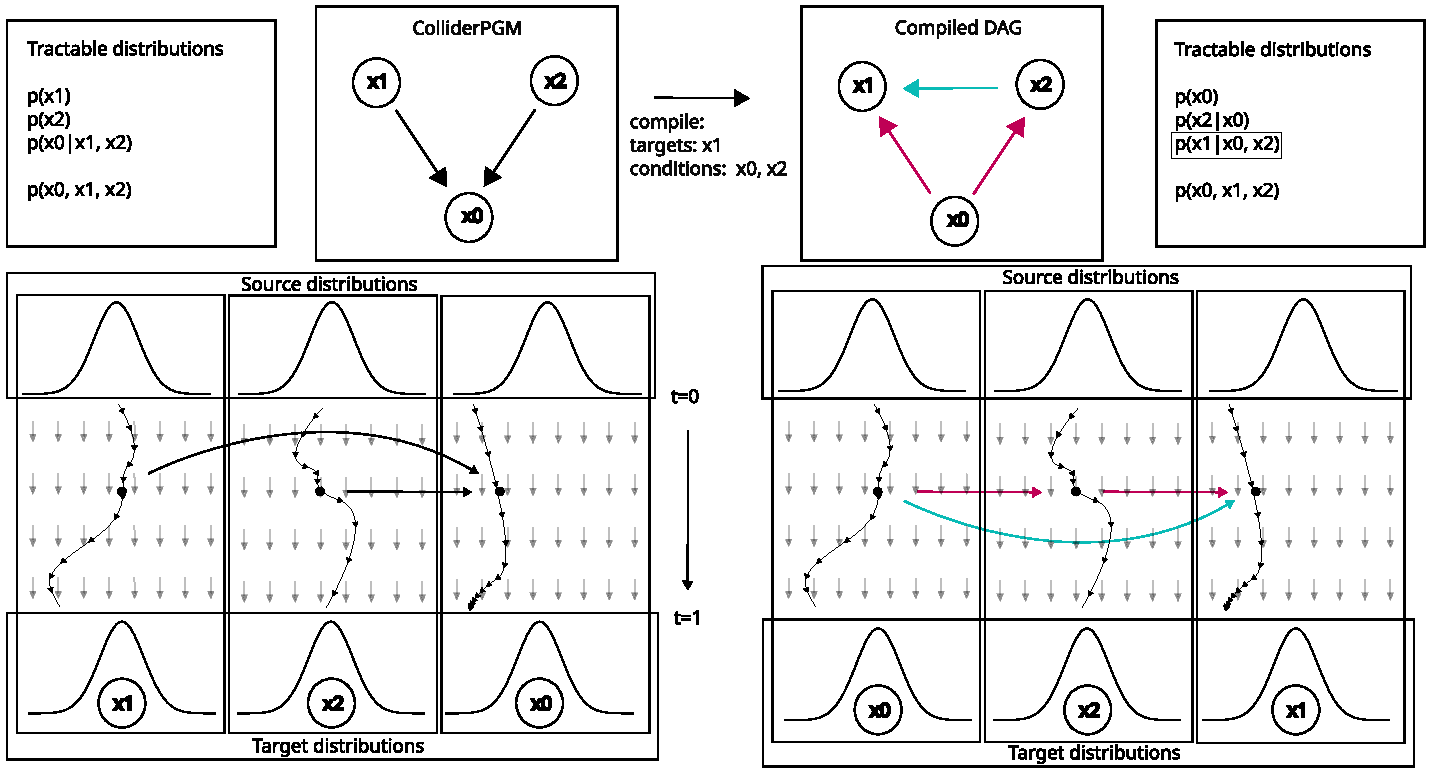
\includegraphics[width=\textwidth]{images/collider-pgm-dual.pdf}
    \caption{\textbf{The StructFlow Pipeline.} Given a causal graph (top, second from left) and an inference query $p(x_1 \mid x_0, x_2)$, StructFlow compiles the graph into a flow architecture. 1. The graph is \textbf{moralized}: because the common effect $x_0$ is observed, its causes $x_1$ and $x_2$ become dependent (``explaining away''), so the compiled DAG gains the teal edge $x_2 \to x_1$. 2. The blocks are ordered with the conditions first ($x_0$, then $x_2$) and the target $x_1$ last, so each block's flow is conditioned on the variables it depends on. The boxes on either side list the distributions each structure makes tractable; below each DAG is its flow, one block per variable, transporting noise (top) to data (bottom).}
    \label{fig:dual-flow}
\end{figure*}

\subsection{Flow Matching Primitives}
Continuous Normalizing Flows (CNFs) transport a simple base density $p_0$ (e.g., $\mathcal{N}(0, I)$) to a complex target $p_1$ along a time-dependent vector field $v_t: \mathbb{R}^d \times [0,1] \to \mathbb{R}^d$: the flow $\phi_t$ solves $\frac{d}{dt}\phi_t(y) = v_t(\phi_t(y))$ with $\phi_0(y) = y$, and integrating from $t=0$ to $1$ carries a sample $y_0 \sim p_0$ to $y_1 = \phi_1(y_0) \sim p_1$. \textbf{Flow Matching} \citep{lipman2022flow} trains the parameterized field $v_t^\phi$ without simulating this ODE, by regressing onto a target conditional field $u_t$ that generates a chosen probability path:
\begin{equation}
    \mathcal{L}(\phi) = \mathbb{E}_{t \sim \mathcal{U}(0,1),\, y_1 \sim p_1,\, y_0 \sim p_0} \left[ \left\| v_t^\phi(y_t) - u_t(y_t \mid y_0, y_1) \right\|^2 \right],
\end{equation}
where, for the linear interpolant, $y_t = (1-t)y_0 + ty_1$ and $u_t(y_t \mid y_0, y_1) = y_1 - y_0$.

\subsection{Block-Triangular Architectures}
\label{sec:block-triangular}

We define a \textbf{Block-Triangular Flow} as a CNF whose velocity field respects a DAG structure $\mathcal{G}$. Let the state $y \in \mathbb{R}^d$ be partitioned into $K$ disjoint blocks $y = [y^{(1)}, \dots, y^{(K)}]$, ordered according to a topological sort of $\mathcal{G}$. The velocity field decomposes as:
\begin{equation}
\frac{d y^{(k)}_t}{dt} = v^{(k)}_\phi\bigl(y^{(k)}_t, \mathrm{Pa}_\mathcal{G}(y^{(k)})_t, t\bigr), \quad k = 1, \dots, K
\end{equation}
where $\mathrm{Pa}_\mathcal{G}(y^{(k)}) \subseteq \{y^{(1)}, \dots, y^{(k-1)}\}$ denotes the parents of block $k$ in the DAG $\mathcal{G}$.

\textbf{Example (Chain).} For $X \to Y \to Z$, block $Z$'s velocity sees $Y$ but not $X$, respecting $Z \perp X \mid Y$.

This constraint ensures the Jacobian $J = \frac{\partial \phi_1(y_0)}{\partial y_0}$ is block lower-triangular, with the log-determinant decomposing as $\log|J| = \sum_{k=1}^K \log|J^{(kk)}|$. This structure enables tractable marginal densities and efficient conditional sampling by fixing parent trajectories. However, this tractability is \emph{asymmetric} and depends strictly on the variable ordering.

The block-triangular structure is realized purely through the connectivity of the velocity network, and it is preserved by the flow dynamics:

\begin{proposition}[Structural Preservation]
\label{prop:structural-preservation}
\rev{Assume velocity fields regular enough for unique, continuously differentiable flows (existence--uniqueness and spatial Lipschitzness, as in \citet{jeong_conditional_2025}, Assumptions~1--2). Parameterize the velocity through a denoiser $\hat{\eta}_1$ under the linear interpolant $y_t = (1-t)y_0 + t y_1$. (i)~If the $k$-th block depends only on the prefix, $\hat{\eta}_1^{(k)}(y, t) = \mathrm{NN}^{(k)}(y^{(1)}, \dots, y^{(k)}, t)$, the induced velocity and flow map are block-triangular and the learned density factorizes autoregressively along the ordering. (ii)~If block $k$ depends only on its graph parents, the jointly-integrated flow map depends on the base noise of $\{k\} \cup \mathrm{Anc}(k)$, refining the conditionals to ancestor sets---ancestral, not yet parental, sparsity. (iii)~Sequential integration with parents resolved to their final values (static conditioning, the causal-mode sampler) sharpens this to the Markov factorization $p(y) = \prod_k p\bigl(y^{(k)} \mid y^{(\mathrm{Pa}(k))}\bigr)$ of $\mathcal{G}$.}
\end{proposition}

This is the architectural guarantee underlying StructFlow (proof in Appendix~\ref{app:proof}): constraining \emph{which inputs each block of the network sees} makes the transport respect the graph, \rev{with the exact granularity---prefix, ancestral, or parental---set by the masking and the integration schedule}. The same structure, however, makes density computation \emph{order-dependent}:

\begin{theorem}[Asymmetry of Marginalization]
\label{thm:marginalization}
In a Block-Triangular Flow with ordering $y^{(1)} \to \cdots \to y^{(K)}$, call the marginal $\log p(y_S)$ of a subset $S$ \emph{directly tractable} if it can be evaluated by the change-of-variables formula restricted to $S$ (a single pass, with no integration over the remaining variables). If $S$ is \emph{ancestrally closed}---contains all parents, and hence all ancestors, of each of its members---then $\log p(y_S)$ is directly tractable; a topological \emph{prefix} $S = \{1, \dots, k\}$ is the canonical such set, and is the case used by our compiler. \rev{Conversely, if $S$ is not ancestrally closed, the restricted formula is invalid for any flow whose missing-ancestor dependencies are functionally non-degenerate (the generic case), and exact evaluation requires marginalizing them out, which is intractable in general.}
\end{theorem}

\textbf{Implication} (proof in Appendix~\ref{app:proof}). This explains why a single fixed architecture cannot efficiently serve both tasks: a causal model ordered $X \to Y$ computes $p(X)$ and $p(X,Y)$ efficiently but must marginalize over $X$ for $p(Y)$, whereas efficient inference $p(X \mid Y)$ needs $Y$ ahead of $X$---a task-specific re-ordering. \rev{Corollary~\ref{cor:query-family} (appendix) makes the supported family explicit: a compilation \emph{samples} $p(T \mid C)$ for every condition-prefix $C$ and arbitrary targets $T$, marginalizing nuisance variables by sampling; \emph{densities} additionally require ancestral closure.}

\subsection{StructFlow: Structural Flow Alignment}
\label{sec:structflow}

A Probabilistic Graphical Model defines a generative factorization of a joint distribution $p(y) = \prod_{k} p(y^{(k)} \mid \mathrm{Pa}(y^{(k)}))$ via a DAG $\mathcal{G}$. We introduce \textbf{StructFlow} (Structural Flow Alignment), an algorithm that translates the abstract graph $\mathcal{G}$ into a concrete block-triangular flow architecture tailored to a specific probabilistic query. Depending on the desired capability, StructFlow produces one of two distinct model artifacts (each trained separately).

Three standard assumptions delimit the queries StructFlow can answer correctly.

\begin{assumption}[Standard causal assumptions]
\label{ass:standard}
(i) \emph{Causal sufficiency:} $\mathcal{G}$ contains no unobserved confounders---every common cause of two variables in $\mathcal{G}$ is itself a node of $\mathcal{G}$. (ii) \emph{Markov condition:} the data distribution factorizes according to $\mathcal{G}$. (iii) \emph{Faithfulness:} every conditional independence in the data distribution is entailed by d-separation in $\mathcal{G}$.
\end{assumption}

Parts (i)--(ii) let the causal-alignment model identify interventional distributions, so that fixing parents in the flow corresponds to a $\mathrm{do}(\cdot)$ operation (Theorem~\ref{thm:level2}). Faithfulness (iii) is used by the inference compiler to prune a candidate dependency whenever the corresponding variables are d-separated, making the compiled inference graph both \emph{sufficient} (no posterior dependency is missed) and \emph{minimal}. We assume $\mathcal{G}$ is known; structure discovery is orthogonal (Section~\ref{sec:future_work}). Counterfactual queries require an additional identifiability condition (Remark~\ref{rem:cf-identifiability}).

\subsubsection{Causal Alignment}
When the goal is mechanistic simulation or causal reasoning, StructFlow preserves the DAG structure directly. The flow blocks are ordered according to a topological sort of $\mathcal{G}$ (roots $\to$ leaves), and each block's velocity field receives inputs only from its DAG parents:
\begin{equation}
    v^{(k)}_\phi(y^{(k)}_t, \mathrm{Pa}_\mathcal{G}(y^{(k)})_t, t)
\end{equation}
Because this structure mirrors the causal mechanisms (respecting the Principle of Independent Mechanisms \citep{Peters2017}), the resulting flow enables interventional queries $p(y \mid \mathrm{do}(x))$ by fixing parent values, and counterfactual queries via flow inversion (Section~\ref{sec:counterfactuals}).

This is more than an analogy: with static conditioning each block reads its parents only through their \emph{terminal} values, so the flow map is literally a system of structural equations driven by independent noise.

\begin{lemma}[The causally-aligned flow is an SCM]
\label{lem:mech-main}
Let $\phi_1$ be the flow map of a causally-aligned StructFlow with static conditioning and a spatially Lipschitz velocity field. Then there exist maps $G_1,\dots,G_K$ such that, for $u \sim p_0$ and
$\hat x = \phi_1(u)$,
\begin{equation}
    \hat x^{(k)} = G_k\bigl(\hat x^{(\mathrm{Pa}_\mathcal{G}(k))},\, u_k\bigr),
    \qquad k = 1,\dots,K,
\end{equation}
with $u_1,\dots,u_K$ mutually independent and each $G_k$ invertible in $u_k$ at fixed parent values, pushing the base block onto the learned conditional $\hat p\bigl(x^{(k)} \mid x^{(\mathrm{Pa}(k))}\bigr)$.
\end{lemma}

This is the $K$-block generalization of Lemma~1 of \citet{jeong_conditional_2025}, and it
licenses the causal reading of the architecture: clamping a block replaces a mechanism rather than conditioning on it. Three consequences follow, proved in
Appendix~\ref{app:hierarchy}: recovering the observational joint recovers \emph{every}
interventional distribution, for arbitrary structural equations, with the interventional
density available in one pass (Theorem~\ref{thm:level2},
Corollary~\ref{cor:interventional-density}); counterfactuals are recovered exactly at the flow-matching optimum whenever each mechanism is monotone coordinate-wise in independent noise or additive, which includes all linear structural equations and our synthetic benchmarks (Theorem~\ref{thm:level3}); and none of this identifies the graph itself---in the linear--Gaussian case every Markov-equivalent DAG
attains the same optimal flow-matching loss while giving different causal answers
(Proposition~\ref{prop:mec}). These guarantees are for static conditioning. Under dynamic conditioning a block reads its ancestors' trajectories, so the learned flow is an SCM on the transitive closure of $\mathcal{G}$ (each parent set replaced by the ancestor set) rather than on $\mathcal{G}$; with the per-block coupling it still targets the correct conditionals, but we do not claim the mechanism-level guarantees for it (Remark~\ref{rem:static-dynamic-equal}).

\subsubsection{Inference Alignment}
When the goal is amortized posterior inference $p(\Theta \mid Y)$ where $\Theta$ are latent variables and $Y$ are observations, StructFlow must address two challenges: \emph{ordering}---by Theorem~\ref{thm:marginalization}, the observations $Y$ must precede the targets $\Theta$ for tractable conditional evaluation---and \emph{posterior dependencies}---the posterior can be \emph{denser} than the prior (at a collider $X_1 \to Y \leftarrow X_2$ with $X_1 \perp X_2$ marginally, observing $Y$ induces $X_1 \not\perp X_2 \mid Y$, a correlation the original DAG has no edge to carry). The compilation pipeline for inference mode consists of three steps:
\begin{enumerate}
    \item \textbf{Moralization:} Connect all pairs of variables sharing a common child in $\mathcal{G}$, then drop edge directions. The posterior is not a causal object---the dependencies conditioning induces (such as the collider coupling above) are symmetric constraints, which the moral graph is guaranteed to contain \citep{Koller2009}.

    \item \textbf{Re-ordering:} Compute a valid ordering where all observations $Y$ precede all targets $\Theta$---not a heuristic but the tractability requirement of Theorem~\ref{thm:marginalization} (within each group we use reverse topological order, which tends to yield sparser parent sets after pruning).

    \item \textbf{Dependency Pruning:} For each target $\theta_k$ in the computed order, determine its minimal parent set using d-separation:
    \begin{equation}
        j \in \mathrm{Pa}_{\text{flow}}(\theta_k) \iff \theta_k \not\perp_d z_j \mid \{z_1, \dots, z_{k-1}\} \setminus \{z_j\},
    \end{equation}
    where $z_1, \dots, z_{k-1}$ precede $\theta_k$. The first two steps overshoot (a complete graph always suffices); the d-separation test removes every dependency the graph refutes, restoring the sparsity that acts as the inductive bias of Appendix~\ref{sec:sample-efficiency}.
\end{enumerate}

The conditioning mechanisms of Section~\ref{sec:conditioning} then operate on this \emph{compiled} graph---the moralized, re-ordered, pruned structure---not on the original DAG. \rev{The two steps divide the work: the dependency set is constructed \emph{entirely} by the d-separation step---explaining-away dependencies between co-parents appear under every conditions-first ordering---while moralization only guides the ordering, toward sparser compiled structures (ablation in Appendix~\ref{app:ordering-ablation}).} Appendix~\ref{app:worked-example} walks the full pipeline through a dense four-node example, including a query for which conditioning and intervening differ, and Appendix~\ref{app:algorithms} gives the explicit algorithms.

\paragraph{One engine per ordering, not per query.} Compilation is specific to a query \emph{class}: a single inference-aligned flow with ordering $[Y, \Theta]$ answers every query whose conditioning set is a prefix of that ordering (the tractable family of Theorem~\ref{thm:marginalization}), for any observed values, without retraining; only a different observation/target split triggers a new compilation and training run. Compilation itself is negligible---$O(K^2)$ d-separation tests, each linear in the size of the graph \citep{Koller2009}---so the dominant cost is flow-matching training, the same cost paid by any CNF of comparable connectivity.

\subsection{Conditioning Mechanisms}
\label{sec:conditioning}

Given a block-triangular flow with ordering $[Y, \Theta]$ (observations first, targets second), we must specify how the target velocity field $v^{(\Theta)}_\phi$---the components governing the evolution of $\Theta$---receives information from the conditioning variables $Y$. We implement two strategies: static conditioning, the standard construction in conditional CNFs and diffusion models (the condition enters as a fixed input), and dynamic conditioning, the recent alternative of \citet{jeong_conditional_2025}.

\paragraph{Static Conditioning.}
In static mode, conditioning variables are first integrated to completion, then their \emph{final values} $y_1 = \phi_1(y_0)$ are provided as fixed inputs to the target velocity field:
\begin{equation}
    \frac{\partial \theta_t}{\partial t} = v^{(\Theta)}_\phi(\theta_t, y_1, t)
\end{equation}
Sampling proceeds sequentially---one ODE solve per block, each block conditioned on the terminal values of its already-integrated parents---so a query with $K$ target blocks requires $K$ sequential solves (observed conditions are fixed values and need none).

\paragraph{Dynamic Conditioning.}
In dynamic mode, all variables are integrated \emph{simultaneously} in a single ODE solve. The target velocity field is conditioned on the \emph{time-evolving trajectory} of the conditioning variables:
\begin{equation}
    \frac{d\theta_t}{dt} = v^{(\Theta)}_\phi(\theta_t, y_t, t)
\end{equation}
where $y_t$ co-evolves with $\theta_t$. This requires the network to learn meaningful representations from partially-noised conditioning variables (at intermediate times $t < 1$), but enables a single parallel ODE integration for all variables. The two mechanisms are contrasted schematically in Appendix Figure~\ref{fig:static-v-dynamic-conditioning}.

\subsection{Counterfactual Inference}
\label{sec:counterfactuals}

Block-triangular flows enable counterfactual reasoning---given an observation $(x, y)$ from a causal model $X \to Y$, answering ``what would $Y$ have been if $X$ had been $x'$?'', formally $p(Y_{x'} \mid X{=}x, Y{=}y)$---via the Abduction-Action-Prediction framework \citep{Pearl2009} (illustrated in Appendix Figure~\ref{fig:counterfactual}). The flow's bijectivity recovers the noise $u$ that generated an observation under the learned model, which allows re-simulation under a hypothetical intervention:

\begin{enumerate}
    \item \textbf{Abduction:} Recover the noise by inverting the flow: integrate $\frac{dy_t}{dt} = -v_t(y_t)$ backward from $y_1 = y_{\text{obs}}$ to obtain $u = \phi_1^{-1}(y_{\text{obs}})$.
    \item \textbf{Action:} Realize $\mathrm{do}(X = x')$ by replacing the natural evolution of $X$ with a fixed trajectory: for static flows, set $x_1 = x'$; for dynamic flows, construct the full trajectory $x'_t$ by integrating backward from $x'$.
    \item \textbf{Prediction:} Integrate $\frac{d\theta_t}{dt} = v^{(\Theta)}_\phi(\theta_t, x'_t, t)$ forward from the \emph{original} noise, $\theta_0 = u_\Theta$, with the intervened variable fixed to its counterfactual trajectory.
\end{enumerate}

\begin{remark}[Counterfactual identifiability]
\label{rem:cf-identifiability}
Abduction recovers the noise $u = \phi_1^{-1}(y_{\mathrm{obs}})$ consistent with the observation \emph{under the learned model}, which is not necessarily the true exogenous noise of the data-generating process. Theorem~\ref{thm:level3} identifies
when the discrepancy is harmless: for a static flow at the flow-matching optimum, if each mechanism is monotone coordinate-wise in independent noise or additive (a class covering all linear structural equations and our synthetic benchmarks), the mismatch is a parent-independent reparameterization that cancels
between abduction and prediction, and the recovered counterfactual is exact. For multivariate blocks that are neither---such as the image block of Section~\ref{sec:colored-mnist}---the condition fails, and those counterfactuals
remain model-based estimates (Remark~\ref{rem:l3-limits}). All of this presumes the graph is
correct; that presumption is the binding one (Proposition~\ref{prop:mec}).
\end{remark}

\section{Experiments and Discussion}
\label{sec:experiments}

Our framework allows us to define a PGM once and compile it into task-specific flows; we evaluate both compiled regimes---\textit{Causal Alignment} for mechanistic queries and \textit{Inference Alignment} for statistical queries---asking whether structure-aligned flows support all three levels of Pearl's causal hierarchy, whether the compiled inference engines provide accurate amortized inference, and how static and dynamic conditioning compare. We compare four methods: \textbf{CAREFL} \citep{khemakhem2021causal}, an affine autoregressive flow baseline; \textbf{Guided}, an unstructured flow trained on the joint and conditioned via reconstruction guidance; and our structure-aligned flows with \textbf{Static} (condition on $x_1$) and \textbf{Dynamic} (condition on $x_t$) conditioning.

\subsection{Experimental Setup}

We train and evaluate on synthetic $4$-node nonlinear PGMs with randomly generated structural equations, giving each model access to samples from the joint distribution (see Appendix~\ref{app:experiments} for details). Graph sizes are bounded by evaluation, not training: the number of supported queries grows rapidly with graph size and every inference-direction query requires its own NUTS ground-truth reference, so we evaluate exhaustively at $n{=}4$ and $n{=}8$ rather than sparsely at larger $n$.

We report the Sliced Wasserstein Distance (SWD) as our primary metric, since the nonlinear PGMs do not admit tractable density evaluation for all queries of interest; it is normalized by $\sqrt{N\,D}$ to be comparable across queries of differing dimension and sample size (so absolute magnitudes are small---the meaningful signal is the \emph{relative} ordering between methods). Where ground-truth densities are available (linear-Gaussian PGMs on causal queries), we additionally report the KL divergence (Appendix~\ref{app:kl-linear}), which corroborates the SWD ranking on a calibrated scale for the methods that define a tractable conditional density (guided sampling does not, so it is scored by SWD only).

\paragraph{Reading the plots.} Box plots aggregate PGM and learner seeds \emph{and all supported conditional queries of each graph}; given the seed counts we report observed spread rather than significance tests. The sharpest claims (moralization, sample efficiency) are measured against exact ground-truth posteriors (Appendix~\ref{app:additional-experiments}).

\subsection{Causal Alignment}

For Causal Alignment, we set the structure of the flow to match the structure of the PGM. This alignment enables the flow to support interventional and counterfactual queries.


\begin{figure*}[t]
    \centering
    \begin{subfigure}[t]{0.32\textwidth}
        \centering
        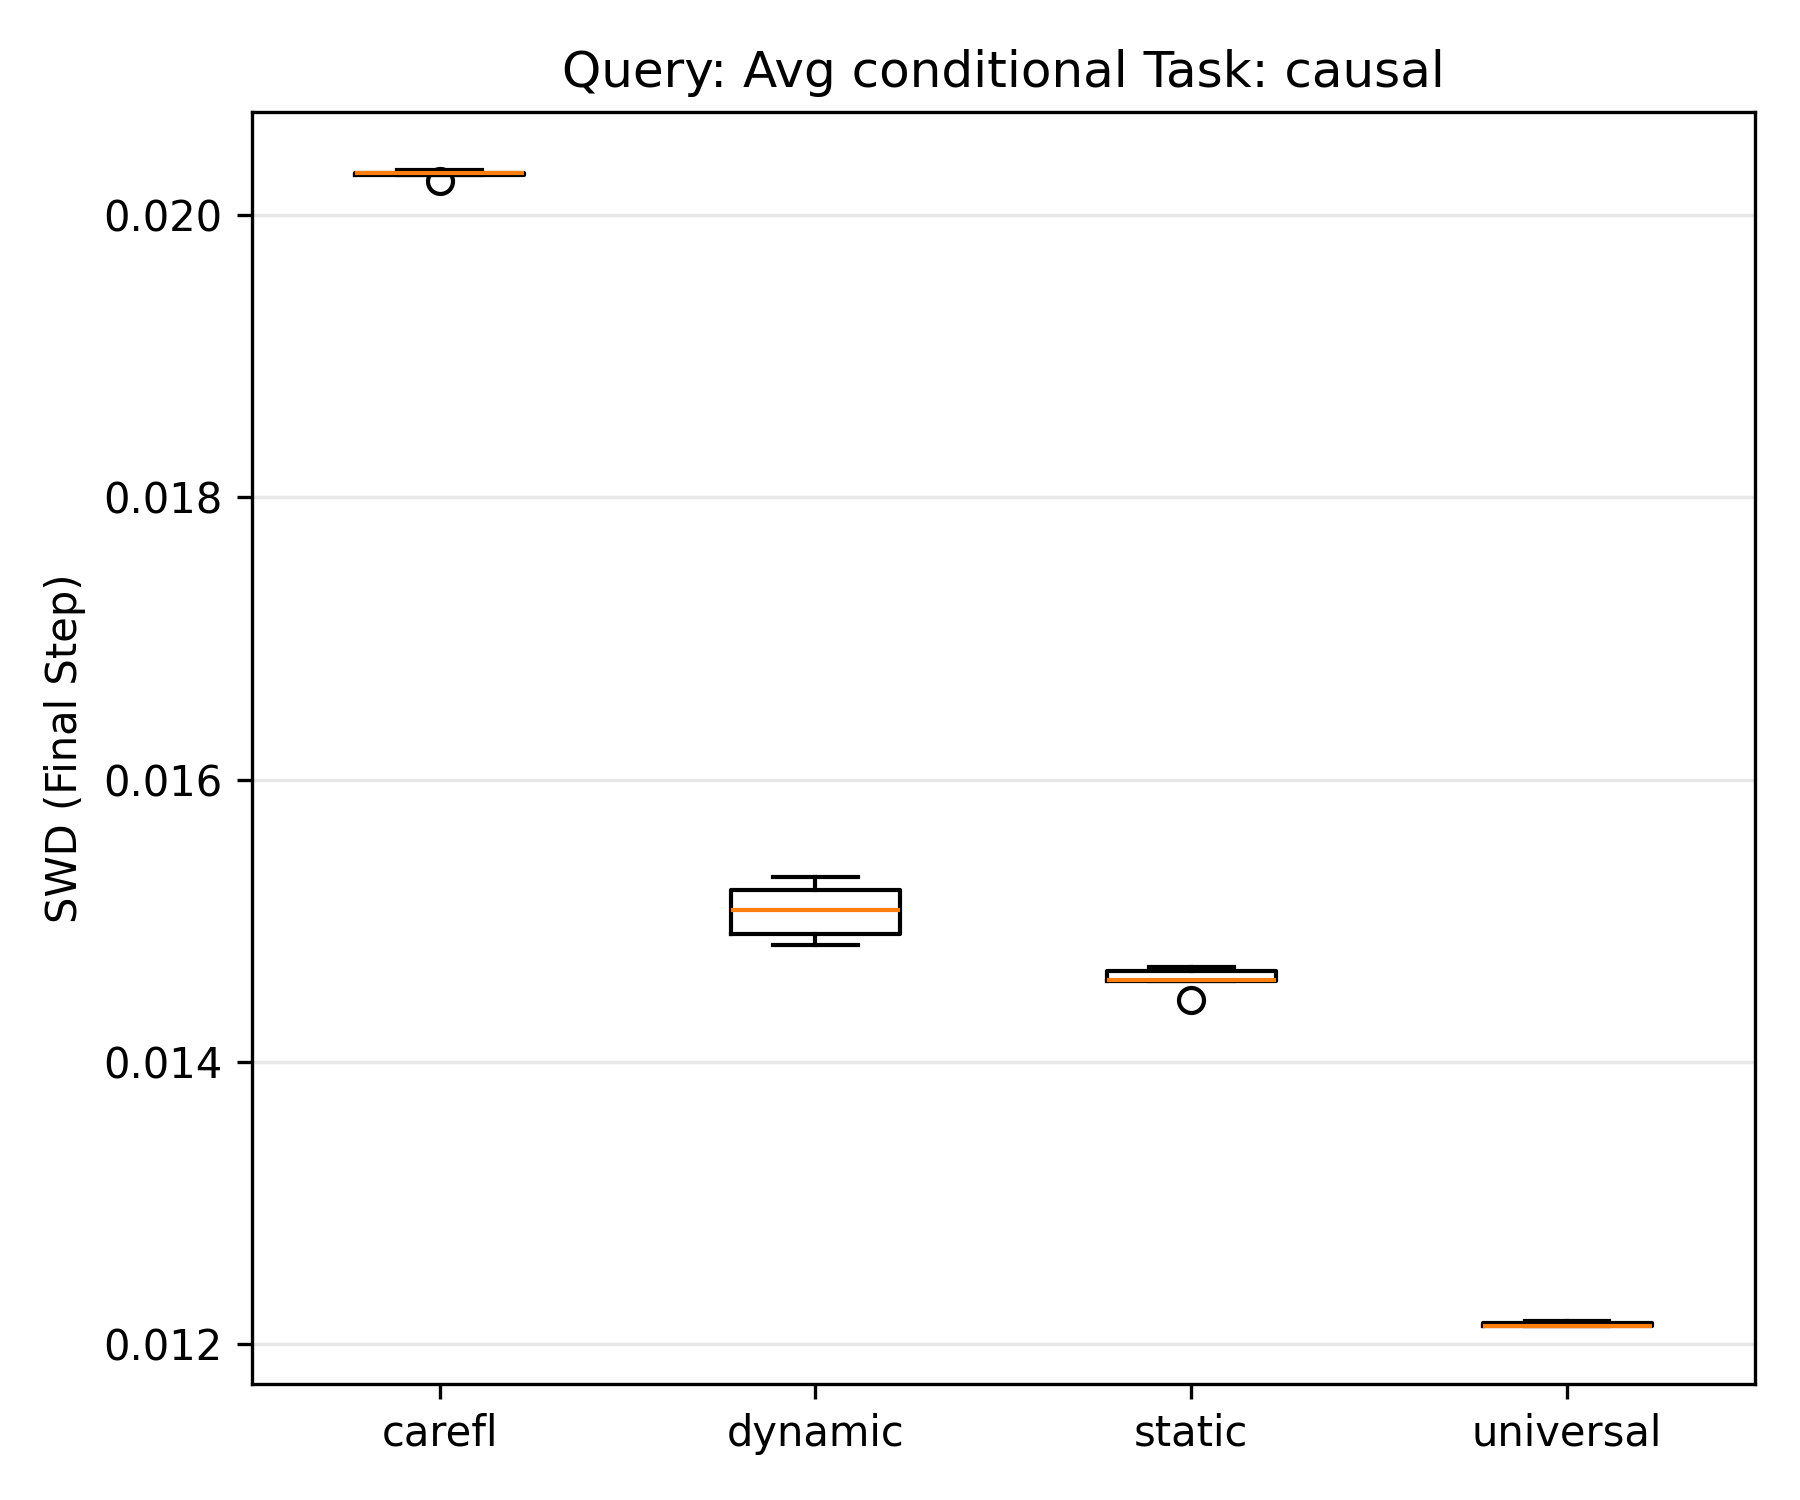
\includegraphics[width=\textwidth]{images/experimental_figures/nonlinear/final_box_swd_pgms_all_task_causal_queries_avg_conditional.png}
        \caption{Interventional $p(y\mid \mathrm{do}(x))$}
        \label{fig:swd-nonlinear-causal}
    \end{subfigure}
    \hfill
    \begin{subfigure}[t]{0.32\textwidth}
        \centering
        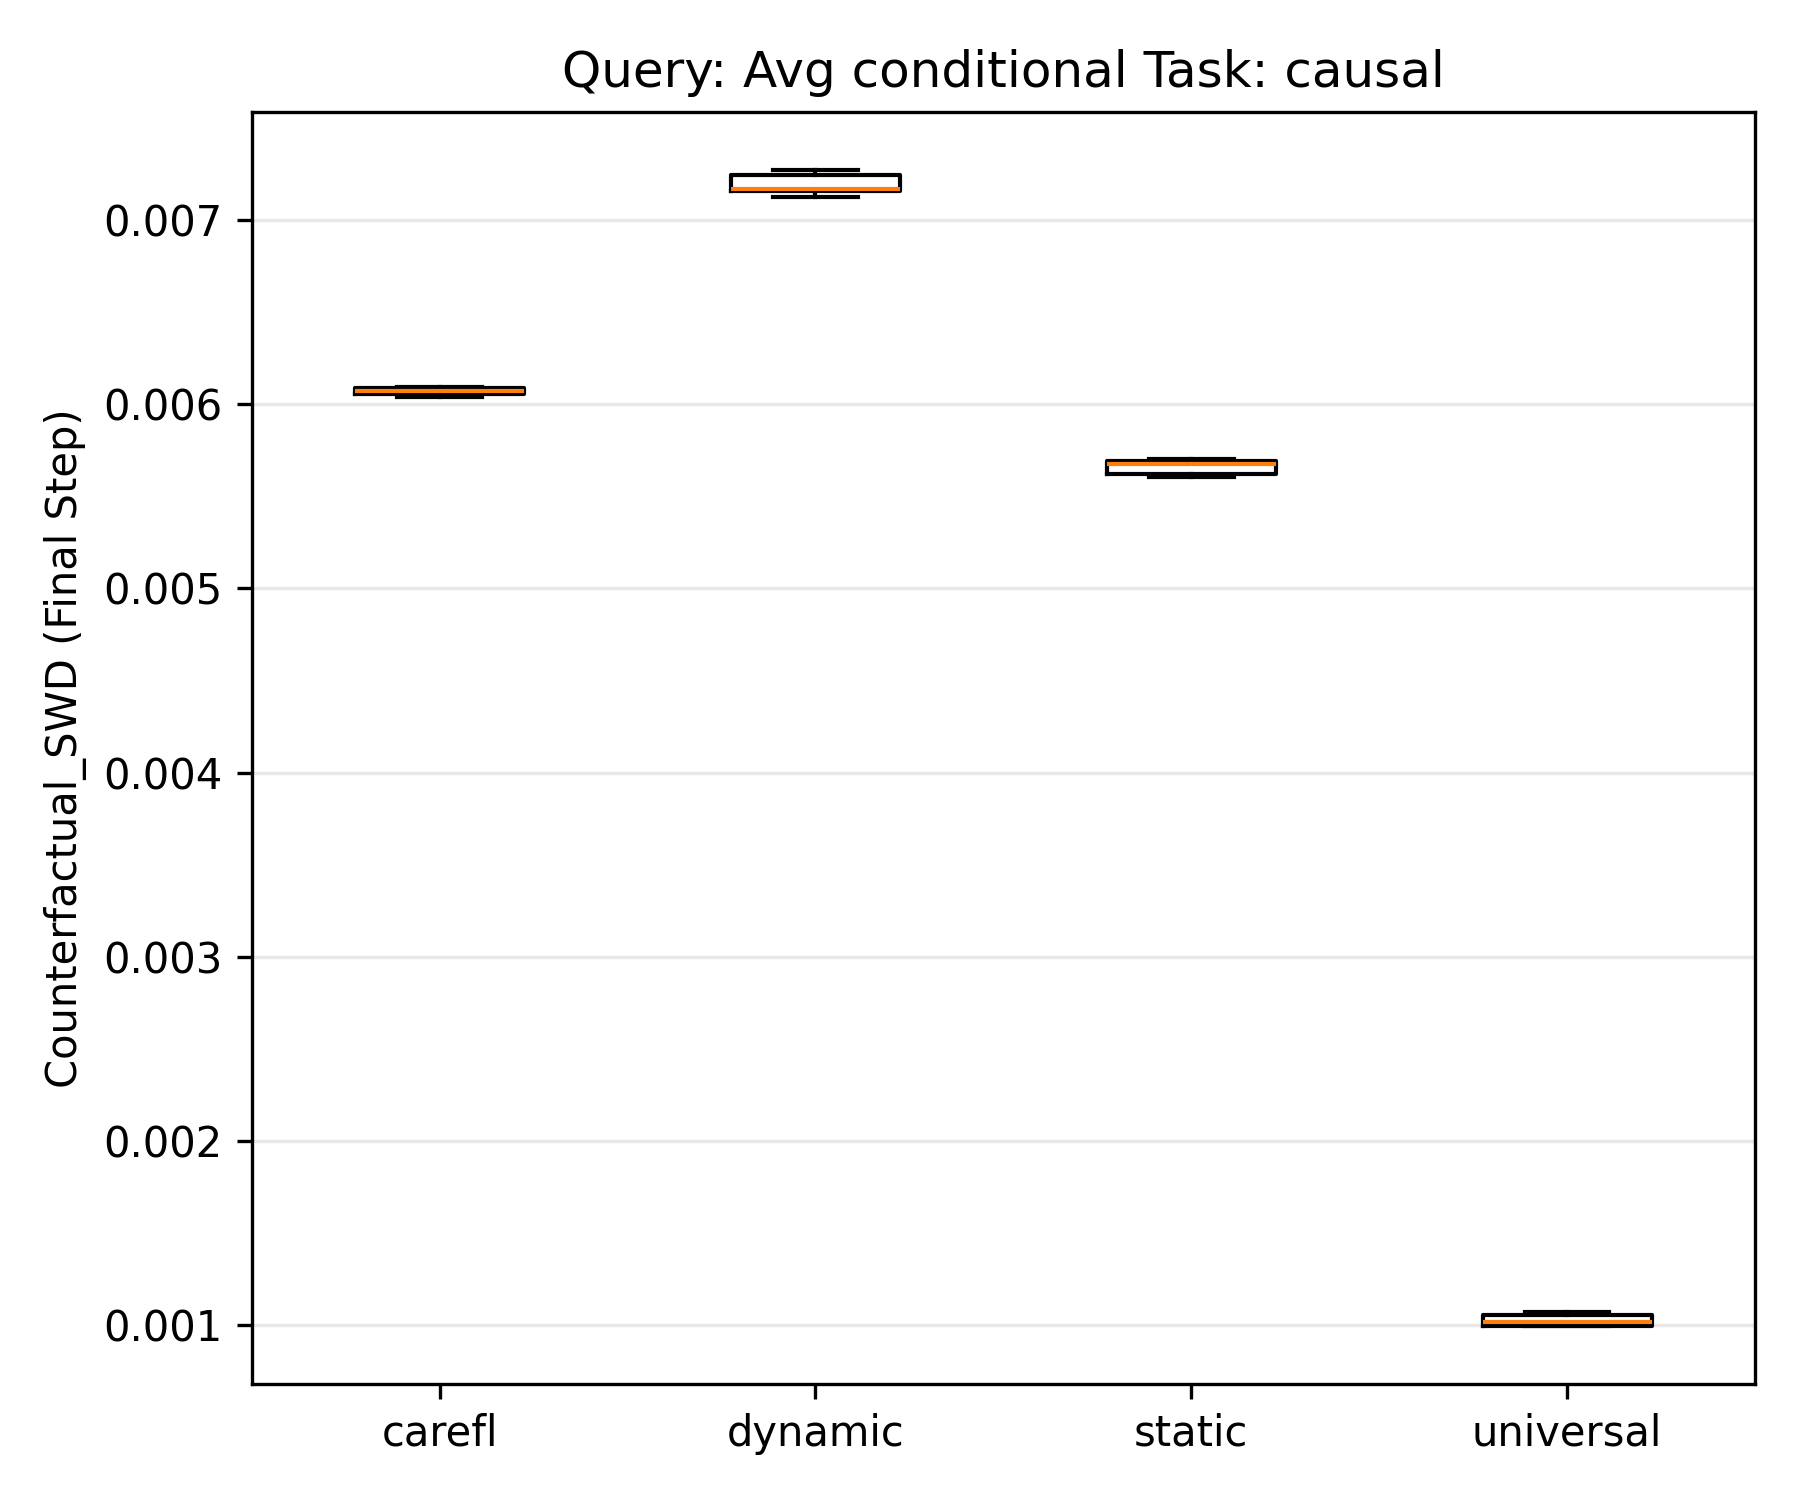
\includegraphics[width=\textwidth]{images/experimental_figures/nonlinear/final_box_counterfactual_swd_pgms_all_task_causal_queries_avg_conditional.png}
        \caption{Counterfactual}
        \label{fig:counterswd-nonlinear-causal}
    \end{subfigure}
    \hfill
    \begin{subfigure}[t]{0.32\textwidth}
        \centering
        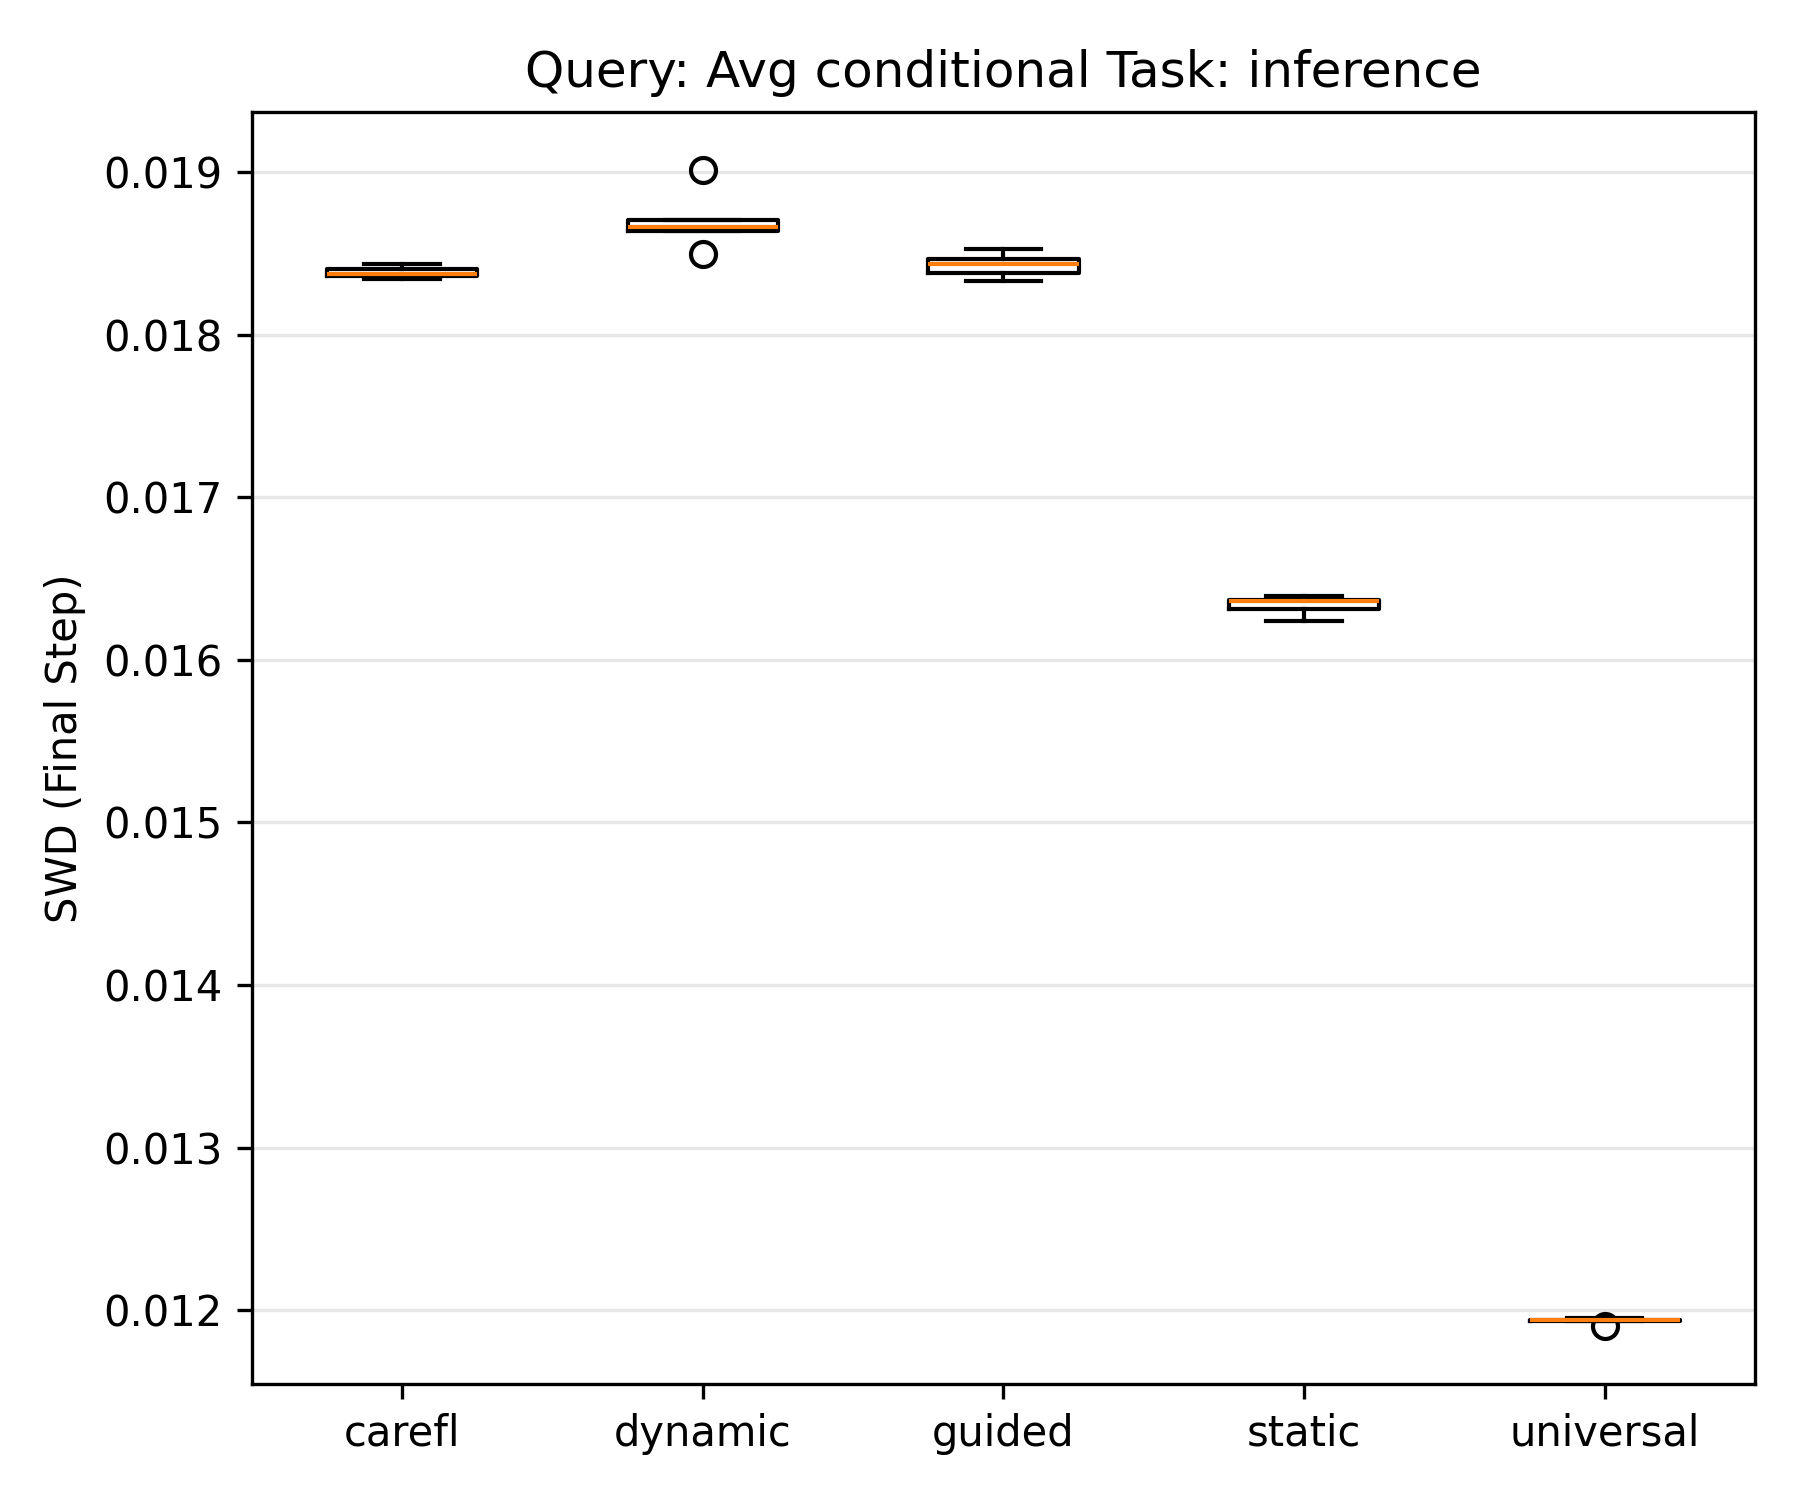
\includegraphics[width=\textwidth]{images/experimental_figures/nonlinear/final_box_swd_pgms_all_task_inference_queries_avg_conditional.png}
        \caption{Inference $p(\mathrm{pa}\mid\mathrm{ch})$}
        \label{fig:inference-nonlinear-pgm}
    \end{subfigure}
    \caption{\textbf{Normalized Sliced Wasserstein Distance on nonlinear 4-node PGMs}, aggregated over the supported conditional queries, 3 PGM seeds and 3 learner seeds. On these nonlinear mechanisms the CNF variants (Static, Dynamic) are competitive with or better than CAREFL on both causal query types (a, b); all methods are comparable on these small, well-sampled inference problems (c). (On the \emph{linear} benchmarks CAREFL's affine class exactly matches the mechanisms and excels, particularly on counterfactuals; Appendix~\ref{app:results}.)}
    \label{fig:pgm-results}
\end{figure*}

\paragraph{Interventional Queries (Level 2).} In the causally aligned flow, an intervention $\mathrm{do}(x)$ is realized by clamping the block of $x$ to the intervened value while integrating all other blocks as usual. The clamped block ignores its own parents, so the flow samples exactly the mutilated graph of the intervention, yielding $p(y \mid \mathrm{do}(x))$. In general this \emph{differs} from the observational conditional $p(y \mid x)$, which additionally updates the distribution of $x$'s ancestors through back-door paths---a task for the inference-aligned model. The two coincide whenever the conditioning set leaves no back-door path to update; two sufficient conditions cover our benchmarks: the conditioning set is \emph{ancestrally closed} (Theorem~\ref{thm:marginalization}; e.g.\ root nodes and topological prefixes), or it contains every direct parent of the target and none of its descendants (both queries then reduce to the same mechanism conditional by the local Markov property). Every causal-mode benchmark query below is of one of these forms.

\paragraph{Counterfactual Queries (Level 3).} Counterfactual queries use the abduction--action--prediction procedure of Section~\ref{sec:counterfactuals}, which requires a bijective correspondence between an observation and the exogenous noise that produced it. Diffusion models with stochastic samplers lack such a correspondence; diffusion-based causal models recover one by replacing the stochastic sampler with a deterministic DDIM or probability-flow-ODE inversion \citep{sanchez2022diffusion, chao2023interventional}---the same flow-inversion principle used here---whereas CNFs provide the bijection natively, alongside exact density evaluation. The two are not equally exact: DDIM inversion carries a first-order abduction bias that a CNF's tolerance-controlled solve does not (Proposition~\ref{prop:abduction-error}; measured in Section~\ref{sec:backbone-ablation}). Recall also that the recovered noise coincides with the \emph{true} exogenous noise only under the conditions of Theorem~\ref{thm:level3}, which cover our synthetic benchmarks (Remark~\ref{rem:cf-identifiability}).

\paragraph{Results.} At the observational level (Level 1), all flow-based methods recover the joint distribution $p(y)$ comparably well, with no consistent separation between structured and unstructured variants (joint-distribution SWD in Appendix Figure~\ref{fig:nonlinear-joint}); we therefore focus the main text on the interventional and counterfactual levels, where structure is load-bearing. Figures~\ref{fig:swd-nonlinear-causal} and~\ref{fig:counterswd-nonlinear-causal} show the comparison on the nonlinear PGMs (per-graph breakdown in Appendix Figure~\ref{fig:swd-linear-v-nonlinear}). On these nonlinear mechanisms, Static and Dynamic match or outperform CAREFL on interventional queries, and all three are close on counterfactuals (Static and CAREFL essentially tied, Dynamic within ${\sim}20\%$). The picture inverts on the \emph{linear} benchmarks (Appendix~\ref{app:results}): there CAREFL's affine transformations coincide exactly with the true mechanism class, and it excels---most visibly on counterfactuals, where abduction through the exactly-matched affine inverse is nearly exact. Both observations are two sides of the same expressivity argument: the affine transformations $x' = s(x_{<i}) \cdot x + t(x_{<i})$ that CAREFL needs for identifiability are not universal density approximators \citep[App.~B--C]{khemakhem2021causal}---exact when the mechanisms are affine, limited when they are not---whereas our CNFs realize any smooth monotone noise-to-value map \citep{zhang2020approximationcapabilitiesneuralodes}. Enforcing causal structure through the \emph{topology} of the vector field rather than the algebraic form of the coupling retains expressivity that affine flows lack.

An ablation replacing each block's velocity field with a per-node denoising diffusion model (the construction of DCM and Diff-SCM) at matched budgets shows the two backbones agree on interventional queries at moderate-to-high NFE while the diffusion variant's abduction error decays only at first order---evidence that the compiled structure, not the choice of continuous-time generative model, is load-bearing (Appendix~\ref{app:additional-experiments}, Section~\ref{sec:backbone-ablation}).

\paragraph{Inference alignment, moralization, and amortization.} Three further results confirm the framework's inference-direction properties and are given in full in Appendix~\ref{app:additional-experiments}: on these small, well-sampled graphs all methods perform amortized posterior inference comparably (Figure~\ref{fig:pgm-results}c); \rev{an ablation on a linear-Gaussian collider shows the compiled co-parent dependency is \emph{necessary}---without it the flow provably cannot represent the induced posterior correlation} (recovered $-0.94$ vs.\ analytic $-0.92$; ablated: $\approx 0$); and the compiled inference engine amortizes, answering posterior queries ${\sim}11\times$ faster than per-query NUTS beyond a crossover of $K^\star \approx 22$ queries.

\subsection{Colored-MNIST: Intervening vs.\ Conditioning \cam{on Images}}
\label{sec:colored-mnist}


\begin{figure}[t]
    \centering
    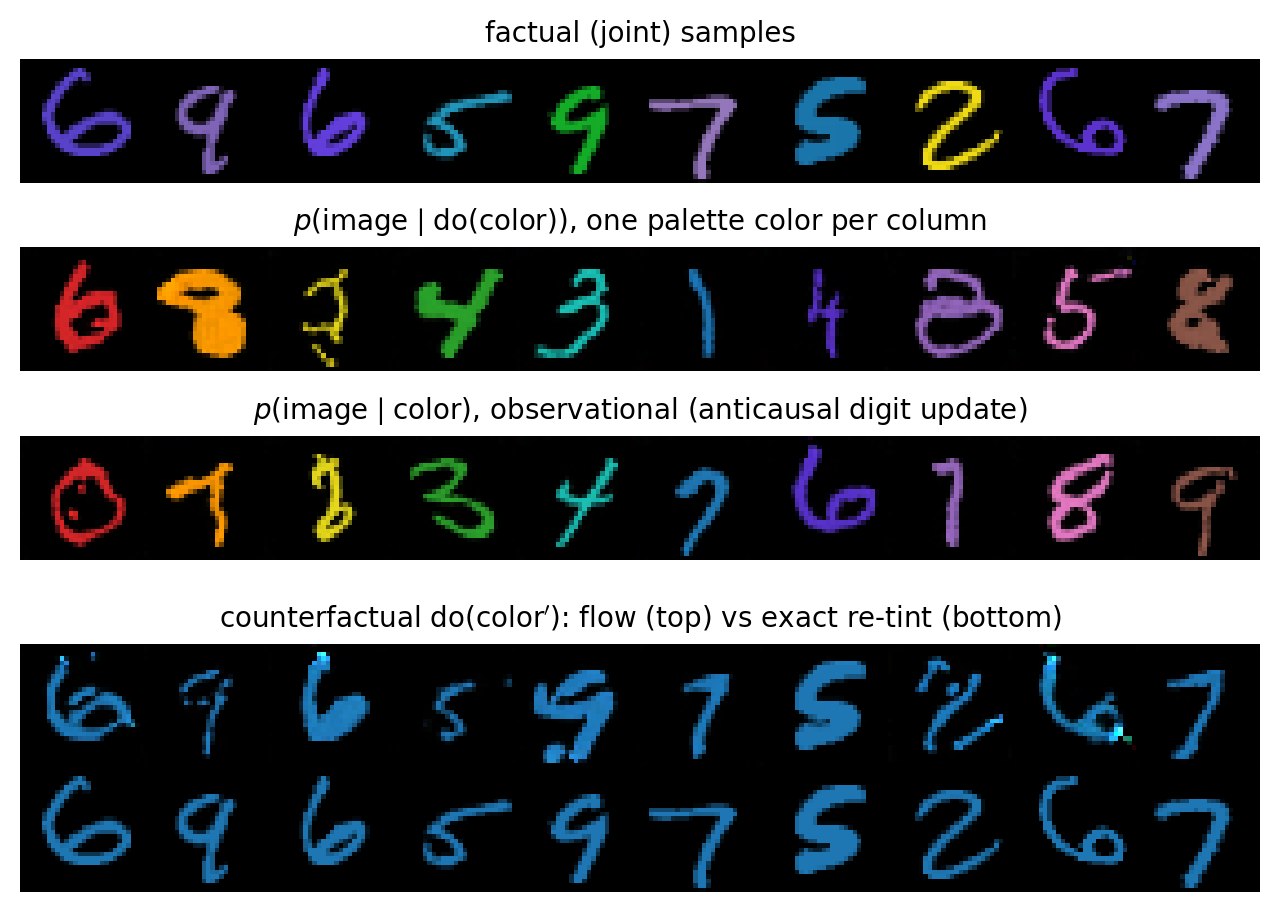
\includegraphics[width=0.44\columnwidth]{images/colored_mnist_conv_strips.png}
    \caption{\textbf{Colored-MNIST samples.} Row 1: factual samples from the joint. Row 2: causal-alignment samples from $p(\mathrm{image} \mid \mathrm{do}(\mathrm{color}{=}\mathrm{palette}_j))$---the forced color does not change which digit appears. Row 3: inference-alignment samples from the observational $p(\mathrm{image} \mid \mathrm{color}{=}\mathrm{palette}_j)$---column $j$ mostly shows its correlated digit $j$. Row 4: counterfactual re-coloring of row 1's factuals under $\mathrm{do}(\mathrm{color}{=}\mathrm{palette}_5)$: the causal flow inverts each image to its exogenous noise and re-generates with the color forced (upper strip); the lower strip is the exact ground truth.}
    \label{fig:colored-mnist-strips}
    \vspace{-1.2\baselineskip}
\end{figure}


The synthetic benchmarks demonstrate non-trivial graph structure at low dimension and MNIST a higher-dimensional problem with trivial structure (Appendix~\ref{app:additional-experiments}); Colored-MNIST combines both, and makes the paper's central distinction---conditioning versus intervening---\emph{visible}. The causal graph is $\text{digit} \to \text{color}$, $(\text{digit}, \text{color}) \to \text{image}$: each digit class has a palette color applied with probability $\rho = 0.8$ (otherwise a uniformly random palette color, plus Gaussian jitter), and the image is the grayscale digit tinted by the color ($28{\times}28{\times}3 = 2352$ dimensions). Because we author this mechanism, the digit posterior $p(d \mid \mathrm{color})$ is available in closed form, and interventional and counterfactual ground truth can be sampled exactly.

From this single specification the compiler produces both artifacts: the causal-alignment model answers $p(\mathrm{image} \mid \mathrm{do}(\mathrm{color}))$ by clamping the color block, while the inference-alignment model (compiled order $[\mathrm{color}, \mathrm{image}, \mathrm{digit}]$) answers the \emph{observational} conditionals, which require the anticausal belief update through $\mathrm{color} \leftarrow \mathrm{digit}$. The block abstraction also gives architectural modularity: any network respecting the block interface (state, parents, time) can serve as a block's velocity field, so we use a small convolutional U-Net for the image block and MLPs for the vector blocks (static conditioning, 8M-parameter budget).

Figure~\ref{fig:colored-mnist-heatmaps} shows the result. Under $\mathrm{do}(\mathrm{color}{=}\mathrm{palette}_j)$ the digit marginal is uniform for every $j$---forcing a color does not change which digit is drawn---and the flow reproduces this. Under \emph{conditioning} on the same color values, the exact posterior concentrates $0.79$ of its mass on the correlated digit, and the flow recovers this diagonal structure ($0.55$--$0.75$ across colors; residual conditional-generation error, not structural---with ground-truth images the flow recovers the exact posterior peak to within $0.02$). The same contrast is visible directly in samples (Figure~\ref{fig:colored-mnist-strips}): under intervention, random digits appear in every color; under conditioning, each color mostly produces its correlated digit. The inference-aligned flow also answers the fully anticausal classification query $p(\mathrm{digit} \mid \mathrm{color}, \mathrm{image})$ with $98.8\%$ held-out accuracy---amortized, with no per-query inference procedure. One honest caveat: at $\rho = 0.8$ the off-palette pairs row 4 produces appear in training with probability ${\sim}2\%$---rare-shot rather than zero-shot. Retraining at $\rho = 1$ removes them entirely and the result is unchanged in kind: interventions extrapolate to every never-seen (digit, color) pair, and counterfactual re-coloring becomes genuinely zero-shot, with residual failures concentrated in abduction (Appendix~\ref{app:colored-mnist-rho1}).

Comparing static and dynamic conditioning on this benchmark (MLP backbone at a matched $8$M budget; mean normalized SWD over $7$--$8$ independently trained runs per mode, seed s.d.\ $\leq 0.3$), both modes answer every compiled query family accurately, with all errors at the $10^{-4}$ scale of the joint-modeling floor. On the joint the two are indistinguishable ($1.7$ vs $1.6 \times 10^{-4}$); on the conditionals dynamic pays a modest relative penalty---$5.3$ vs $1.7 \times 10^{-4}$ on the causal $p(\mathrm{image} \mid \mathrm{digit}, \mathrm{color})$ and $7.8$ vs $1.9 \times 10^{-4}$ on the observational $p(\mathrm{image} \mid \mathrm{color})$, i.e.\ $3$--$4\times$---consistent with the depth-and-informativeness mechanism of Section~\ref{sec:chain-stiffness}.


\subsection{Scaling Dynamic Conditioning: The Price of Parallelism}
\label{sec:chain-stiffness}

The results above leave static and dynamic conditioning competitive, and dynamic additionally samples all blocks in a single parallel ODE solve. Is that parallelism a free win? At sampling time, dynamic conditioning clamps observed conditions to a trajectory integrated backward from the observed value; we stress-test how this scales with the depth of nested dependencies on chains $x_0 \to \cdots \to x_{n-1}$, conditioning on the leaf and inferring the root---the query whose conditioning signal must propagate deepest. Since any stationary chain's root--leaf correlation decays geometrically---deep chains would become easy-to-fake tasks with vanishing headroom over the prior---we use a unit-root random walk, $x_{k+1} = x_k + \sigma\varepsilon_k$ with $\sigma = 0.2$ and $x_0 \sim \mathcal{N}(0,1)$: each link is near-deterministic (conditional s.d.\ $0.2$ against unit-scale marginals) yet the root--leaf correlation $1/\sqrt{1 + (n{-}1)\sigma^2}$ decays only polynomially, still $0.67$ at $n{=}32$. We train both modes at matched parameter budgets for $n \in \{2, 4, 8, 16, 32\}$ and measure the $2$-Wasserstein distance to the exact Gaussian posterior (Figure~\ref{fig:chain-stiffness}).

At a matched solver budget (Figure~\ref{fig:chain-stiffness}, left; equal step counts give the two modes near-equal FLOPs, static's $n$ small-block solves matching dynamic's full-network evaluations), static error grows slowly and monotonically with depth ($0.19$ to $0.52$) as its sequential block solves accumulate error, staying well below the prior baseline throughout. Dynamic starts ${\sim}2.8\times$ worse and \emph{degrades} with depth, until at $n{=}32$ its error ($0.88 \pm 0.14$) exceeds that of ignoring the evidence entirely ($0.65$)---conditioning has become actively harmful. Three diagnostics locate the failure. \emph{First}, static \emph{converges} with solver effort (error flat beyond ${\sim}32$ RK4 steps at every depth), whereas dynamic \emph{anti-converges}---error \emph{increases} with solver accuracy ($0.72$ at $4$ steps to $0.96$ at $128$ for $n{=}32$): faithfully integrating a velocity field evaluated off-distribution amplifies its error, and coarse integration acts as accidental regularization. \emph{Second}, the source: the clamped condition trajectory leaves the training distribution---its $z$-score against the training-interpolant marginal grows from $6.7$ at $n{=}4$ to $86$ at $n{=}32$ under an informative ($90$th-percentile) observation---because deeper evidence is more informative, landing the backward integration off the manifold the network was trained on. \emph{Third}, the naive hypothesis---depth makes the dynamic ODE stiffer---fails instructively: peak velocities do grow with depth ($2.9\times$ the unconditional level at $n{=}2$ to $41\times$ at $n{=}32$) but \emph{only at the clamped condition block}, whose velocity is discarded at every step: a futile corrective response, and a pure OOD diagnostic. The integrated blocks stay at $2$--$4\times$ (static's ${\sim}1\times$)---the learned dynamics never stiffen; the error enters through the conditioning trajectory itself. The same grading appears in the paper's own benchmarks: on the $8$-node linear graphs, dynamic's conditional error relative to static grows with the number of conditioning variables ($3.1\times$ at one to $11.4\times$ at five or more), while static, CAREFL, and the unstructured baselines remain flat. The practical reading: dynamic's parallelism is paid for in error that is \emph{structural}---growing with the depth and informativeness of the evidence, an order of magnitude noisier across seeds, not repairable by solver effort---marking the conditioning trajectory itself as the object to fix (Section~\ref{sec:future_work}); static's error is solver-converged and predictable, responding to the knobs a practitioner controls.

\paragraph{Relation to language-model decoding.} The static/dynamic split mirrors the autoregressive-vs-diffusion divide in language models: static is ancestral sampling in a compiled order; dynamic parallels diffusion-LM decoding, where all positions co-evolve and prompt tokens are clamped during the reverse process. The failure modes translate: parallel decoding's error is likewise mechanism-set---within-step tokens commit independently, and sequence-level correctness needs steps scaling with length \citep{liu2024copula,feng2025theoretical}---and \emph{inaccurate} sampling has flattered masked-diffusion metrics much as coarse integration flatters dynamic \citep{zheng2024masked}. Off-manifold clamping is documented for \emph{continuous}-state diffusion \citep{lugmayr2022repaint,ning2023input}---our chains isolate a stronger form, injected purely through the conditioning trajectory even for a perfect model---while masked \emph{discrete} diffusion escapes it, clamped tokens staying on the training manifold \citep{ou2024absorbing}. Where adaptive token order is decisive for masked diffusion \citep{kim2025train}, our inference alignment chooses it at compile time.

\begin{figure*}[t!]
    \centering
    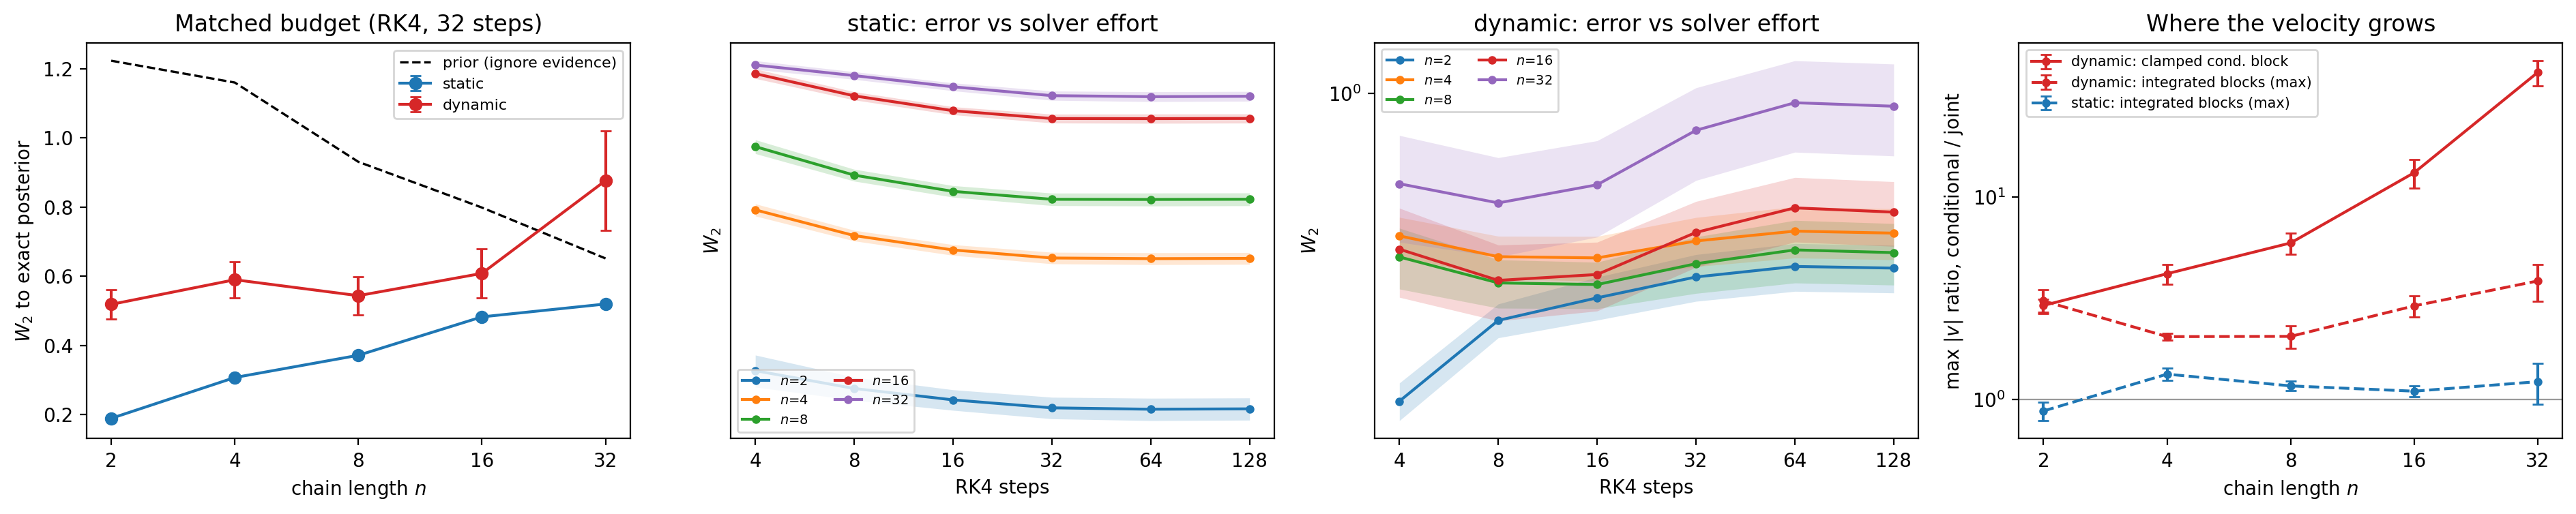
\includegraphics[width=0.93\textwidth]{images/ablations/chain_stiffness_rw.png}
    \caption{\textbf{Scaling dynamic conditioning on chains.} $W_2$ to the exact posterior of $p(x_0 \mid x_{n-1})$ on unit-root random-walk chains; $25$ evidence draws per depth, bands $\pm 1$ s.d.\ over $8$ seeds. \textbf{Far left:} matched budget ($32$ RK4 steps ${\approx}$ equal FLOPs): static grows slowly and monotonically; dynamic starts ${\sim}2.8\times$ worse, degrades with depth, and at $n{=}32$ crosses the dashed prior baseline (ignoring the evidence). \textbf{Middle:} static converges with step budget; dynamic \emph{anti-converges}. \textbf{Far right:} only the clamped condition block's velocity amplification grows with depth---the learned dynamics never stiffen.}
    \label{fig:chain-stiffness}
    \vspace{-0.8\baselineskip}
\end{figure*}
\section{Future Work and Limitations}
\label{sec:future_work}

\paragraph{\cam{Scope and real-world applicability.}}
\cam{Our experiments establish the compiler's behaviour where answers can be checked: synthetic graphs with exact or MCMC ground truth (up to $n{=}8$ nodes, $64$ dimensions), plus MNIST and Colored-MNIST, where the image block is high-dimensional but the graph has two or three nodes. None of these is a real-world system, and we make no claim about performance on one. Real applications add three difficulties that our benchmarks deliberately exclude: the graph must be estimated rather than given (next paragraph), causal sufficiency may fail through hidden confounding, and graphs with many high-dimensional nodes stress both training and, more severely, evaluation (``Scaling to Large PGMs'' below). Applying StructFlow to, e.g., simulators in the sciences with known mechanistic structure, where ground truth is partially available, is the natural next test.}

\paragraph{Known structure.}
Structure discovery is out of scope: the compiler consumes a given DAG, and Appendix~\ref{app:hierarchy} delimits what is provably recovered under it---every interventional distribution for arbitrary mechanisms (Theorem~\ref{thm:level2}), exact counterfactuals for invertible-in-noise or additive mechanisms (Theorem~\ref{thm:level3})---and what is not: the graph itself is unrecoverable from observational data in the linear--Gaussian case (Proposition~\ref{prop:mec}), while for linear non-Gaussian (LiNGAM) models all three levels of Pearl's hierarchy follow end-to-end (Corollary~\ref{cor:lingam}). Coupling StructFlow to a structure learner---and studying degradation under a mis-specified graph---is the highest-value extension.

\paragraph{Counterfactual densities under partial observation.}
Corollary~\ref{cor:interventional-density} gives the interventional \emph{density} in a single pass. The counterfactual analogue only exists under \emph{partial} observation (fully-observed abduction leaves a point mass), and evaluating it requires the inference-aligned artifact alongside the causal one (Remark~\ref{rem:density-scope}); making the two artifacts cooperate on this query is a natural next step.

\paragraph{Scaling to Large PGMs.}
We evaluate exhaustively on small PGMs; the binding constraint is the cost of \emph{ground truth}, not training. The two compilations of a dense $n$-node graph jointly support ${\sim}n^2$ tractable queries (already $72$ at $n{=}8$), and every inference-direction query needs its own long NUTS reference chain at every evaluated conditioning value---this evaluation cost, not model capacity, stops our benchmarks at $n = 8$; how performance scales with graph size remains open.

\paragraph{Backbone Comparison Scope.}
The backbone ablation (Appendix~\ref{app:additional-experiments}) swaps the per-block primitive under matched budgets, isolating the compiled structure's contribution; it is \emph{not} a benchmark against modern diffusion practice---samplers, schedules, distillation, and guidance would all narrow the low-NFE gap we measure, and CNFs have accelerations we equally omit; conclusions about backbones concern the un-augmented primitives only.

\paragraph{Repairing Dynamic Conditioning at Depth.}
\cam{Section~\ref{sec:chain-stiffness} separates two errors of dynamic conditioning. The first, the bias of the block-triangular optimum, is removed by the per-block coupling. The second, a learning error that grows with depth while the coupling alone would allow far less, remains open. Natural next steps are to determine how it scales with model capacity and training length, to use couplings closer to the exact Knothe--Rosenblatt map than a batch-$128$ matching, and to use hybrid schedules that switch from dynamic to static conditioning as $t \to 1$.}

\section{Conclusion}

We presented \textbf{StructFlow}, a methodology for compiling Probabilistic Graphical Models into task-specific Block-Triangular Flows: a \textit{Causal Alignment} model preserving the generative factorization for interventional and counterfactual queries, or an \textit{Inference Alignment} model capturing posterior correlations.

\cam{Our evidence comes from synthetic graphs and image benchmarks with checkable answers; real-world applicability remains to be demonstrated (Section~\ref{sec:future_work}).} Two conclusions follow. First, the compiler abstraction earns its keep: one specification compiles to answer interventional, counterfactual, and amortized posterior queries correctly \rev{(co-parent dependencies for colliders; tractable prefix queries)}. Second, static and dynamic conditioning are competitive on our benchmarks, but dynamic's parallel sampling is not free: on deep chains its clamped trajectories leave the training distribution, and solver effort amplifies rather than repairs its error (Section~\ref{sec:chain-stiffness}).


% % Acknowledgements should only appear in the accepted version.
% \section*{Acknowledgements}

% \textbf{Do not} include acknowledgements in the initial version of the paper submitted for blind review.

% If a paper is accepted, the final camera-ready version can (and usually should) include acknowledgements.

\section*{Broader Impact Statement}

StructFlow is methodological: it provides tooling for answering causal and probabilistic queries under a user-specified graphical model. The principal risk of such tooling is over-trust: every conclusion inherits the assumptions of Section~\ref{sec:structflow} (a correct, causally sufficient graph), and interventional or counterfactual outputs computed under a mis-specified graph can lend unwarranted causal authority to spurious conclusions in high-stakes settings such as medicine or policy. We state these assumptions explicitly and recommend sensitivity analysis to graph mis-specification before any decision-relevant use. Beyond this, we foresee no risks specific to our method above those common to generative modeling.

\section*{Reproducibility Statement}

All theoretical claims are accompanied by proofs: Theorem~\ref{thm:marginalization} and Propositions~1--3 are proved in Appendix~\ref{app:proof}, and the compilation procedure is given as explicit algorithms in Appendix~\ref{app:algorithms}. The PGM-to-flow compiler, the static/dynamic/guided conditioning mechanisms, and all benchmarks are implemented in a single open-source library\cam{, released at \url{TODO-PUBLIC-REPO-URL} (the version tagged \texttt{tmlr-camera-ready} reproduces every result in this paper, including the bug fixes and re-runs described in Appendix~\ref{app:coupling})}. Each analysis experiment is reproduced by a self-contained script with fixed seeds---the moralization ablation (Section~\ref{sec:moralization-ablation}), the sample-efficiency sweep (Section~\ref{sec:sample-efficiency}), and the amortization comparison (Section~\ref{sec:amortization}). The synthetic PGM benchmarks (Section~\ref{sec:experiments}) are generated from fixed seeds, and the exact architectures, optimizer settings, and parameter-budgeting procedure are documented in Appendix~\ref{app:implementation}. Ground-truth posteriors are computed in closed form where available (linear-Gaussian models) and via the No-U-Turn Sampler otherwise; the NUTS references are validated by closed-form anchors, warmup-sensitivity checks, and simulation-based calibration (Appendix~\ref{app:nuts-validation}).

\newpage
\bibliographystyle{tmlr}
\bibliography{references}

%%%%%%%%%%%%%%%%%%%%%%%%%%%%%%%%%%%%%%%%%%%%%%%%%%%%%%%%%%%%%%%%%%%%%%%%%%%%%%%
%%%%%%%%%%%%%%%%%%%%%%%%%%%%%%%%%%%%%%%%%%%%%%%%%%%%%%%%%%%%%%%%%%%%%%%%%%%%%%%
% APPENDIX
%%%%%%%%%%%%%%%%%%%%%%%%%%%%%%%%%%%%%%%%%%%%%%%%%%%%%%%%%%%%%%%%%%%%%%%%%%%%%%%
%%%%%%%%%%%%%%%%%%%%%%%%%%%%%%%%%%%%%%%%%%%%%%%%%%%%%%%%%%%%%%%%%%%%%%%%%%%%%%%
\newpage
\appendix

\section*{Appendix}

\section{Appendix: StructFlow Details}
\label{app:compiler}

We provide the implementation details for Inference Alignment of a DAG.

\begin{figure*}[hbt!]
    \centering
    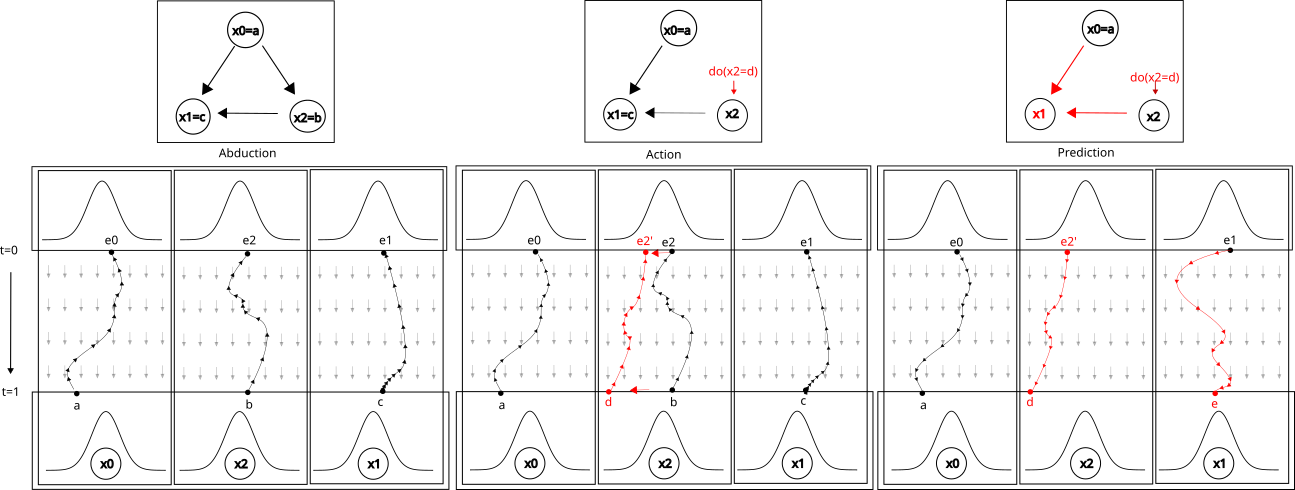
\includegraphics[width=\textwidth]{images/collider-counterfactual.png}
    \caption{\textbf{Counterfactual Inference via Flow Inversion.} To answer ``What would $Y$ have been if $X$ had been $x'$?'', we perform three steps. \textbf{(1) Abduction:} Integrate backward from the observation $(x, y)$ to recover the exogenous noise $u = (u_X, u_Y)$. \textbf{(2) Action:} Construct the intervention trajectory $x'_t$ (red path) by integrating backward from $x'$. \textbf{(3) Prediction:} Integrate forward using the original noise $u_Y$ but conditioned on the intervention trajectory $x'_t$. The result $y_{\text{cf}}$ is the counterfactual outcome---what $Y$ would have been for this specific individual under the hypothetical intervention.}
    \label{fig:counterfactual}
\end{figure*}

\subsection{Algorithm}
The compilation process consists of three stages: Validation, Ordering, and Dependency Resolution.

\paragraph{1. Validation}
The compiler first verifies that the requested query is well-posed.
\begin{itemize}
    \item \textbf{Variable Validity:} Targets $\Theta$ and Conditions $Y$ must be valid subsets of the PGM variables.
    \item \textbf{Disjoint Sets:} Targets $\Theta$ and Conditions $Y$ must be disjoint.
\end{itemize}

\paragraph{2. Variable Ordering}
To construct a valid flow, we must order the variables $[z_1, \dots, z_K]$ such that no variable depends on a future one.
\begin{algorithm}[H]
\caption{Variable Ordering Scheme}
\begin{algorithmic}
\STATE \textbf{Input:} PGM Dag $\mathcal{G}$, Conditions $Y$
\STATE \textbf{Output:} Ordered List $\mathcal{O}$
\STATE Compute Topological Sort $\mathcal{T}$ of $\mathcal{G}$
\STATE Construct Moral Graph $\mathcal{G}_m$ from $\mathcal{G}$
\STATE Sort $Y$ by decreasing index in $\mathcal{T}$ (Reverse Topological)
\STATE Initialize $\mathcal{O} = Y$, Queue $Q = Y$
\WHILE{$Q$ is not empty}
    \STATE $u \gets Q$.pop()
    \STATE Get neighbors of $u$ in $\mathcal{G}_m$, sort by decreasing index in $\mathcal{T}$
    \FOR{neighbor $v$ in sorted neighbors}
        \IF{$v \notin \mathcal{O}$}
            \STATE append $v$ to $\mathcal{O}$ and $Q$
        \ENDIF
    \ENDFOR
\ENDWHILE
\STATE Append remaining nodes from $\mathcal{T}$ in reverse order
\STATE \textbf{return} $\mathcal{O}$
\end{algorithmic}
\end{algorithm}
We prioritize placing conditioning variables first so they can serve as fixed inputs, sorting them by reverse topological order. The subsequent BFS on the moral graph (exploring neighbors in reverse topological order) ensures that strongly coupled variables are grouped together, while the final reverse topological sort respects the dependencies of any remaining unconditioned sub-structures.

\paragraph{3. Dependency Pruning}
For every block $z_k$ in the computed order, we determine its parent set $\text{Pa}(z_k)$ using the d-separation criterion available in network analysis tools (e.g., NetworkX).
\begin{equation}
    j \in \text{Pa}(z_k) \iff z_k \not\perp_{d} z_j \mid \{z_1, \dots, z_{k-1}\} \setminus \{z_j\}
\end{equation}
This step ensures strict minimality of the flow's dependency graph.

\subsection{Worked Example: Compiling a Dense Four-Node Graph}
\label{app:worked-example}

We walk the full pipeline through the DAG $\mathcal{G}$ with nodes $\{Z_1, X, Z_2, Y\}$ and edges
$Z_1 \to X$, $Z_1 \to Y$, $Z_1 \to Z_2$, $X \to Y$, $X \to Z_2$, $Z_2 \to Y$
(topological order $[Z_1, X, Z_2, Y]$), for one query of each kind: the posterior $p(z_2 \mid x, y)$ and the interventional $p(y \mid \mathrm{do}(x))$. Figure~\ref{fig:worked-example} shows each stage; all orderings and dependency sets below are the verbatim output of our compiler on this graph.

\begin{figure*}[hbt!]
    \centering
    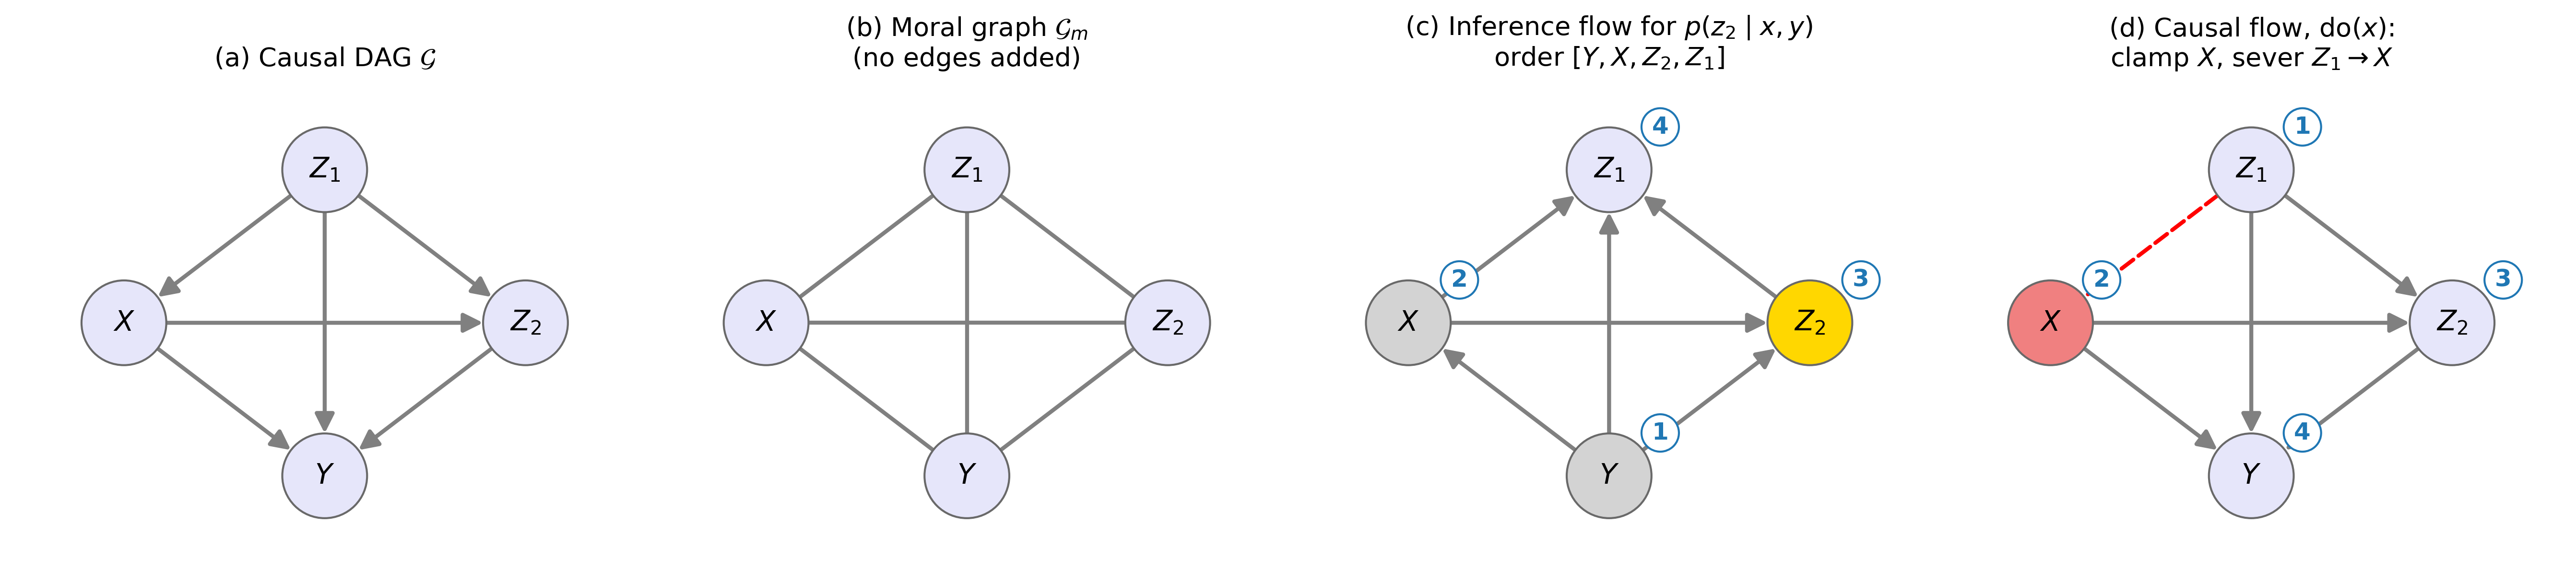
\includegraphics[width=\textwidth]{images/worked_example_compilation.png}
    \caption{\textbf{Worked example of the compiler.} \textbf{(a)}~The causal DAG $\mathcal{G}$. \textbf{(b)}~Its moral graph $\mathcal{G}_m$: every pair of parents sharing a child is already adjacent, so moralization adds no edge here (contrast Figure~\ref{fig:dual-flow}, where it does). \textbf{(c)}~The inference-aligned flow compiled for $p(z_2 \mid x, y)$: conditions $X, Y$ (gray) precede the target $Z_2$ (gold); the marginalized $Z_1$ is ordered last and is never sampled for this query. Circled numbers give the block order. \textbf{(d)}~The causal-aligned flow answering $p(y \mid \mathrm{do}(x))$: the block of $X$ is clamped (red), severing the edge $Z_1 \to X$ (dashed), while $Z_1$ is integrated from its prior.}
    \label{fig:worked-example}
\end{figure*}

\paragraph{Query 1: $p(z_2 \mid x, y)$ (Inference Alignment).}
The conditions are $\{X, Y\}$ and the target is $\{Z_2\}$; the remaining variable $Z_1$ is neither, and must be marginalized.
\emph{Moralization:} the parents of $Y$ ($\{Z_1, X, Z_2\}$) and of $Z_2$ ($\{Z_1, X\}$) are married pairwise; in this dense graph every such pair is already adjacent, so no edge is added and the moral graph $\mathcal{G}_m$ is the complete graph on the four nodes. (Figure~\ref{fig:dual-flow} shows the complementary case of a bare collider, where moralization does add an edge.)
\emph{Re-ordering:} the conditions come first, sorted in reverse topological order, giving $[Y, X]$; the breadth-first traversal of $\mathcal{G}_m$ then appends $Z_2$ and finally $Z_1$, so $\mathcal{O} = [Y, X, Z_2, Z_1]$. Note that the marginalized variable $Z_1$ lands \emph{after} the target: the prefix $\{Y, X, Z_2\}$ is ancestrally closed in the compiled graph, so by Theorem~\ref{thm:marginalization} the flow marginalizes $Z_1$ for free---it is simply never sampled.
\emph{Pruning:} every candidate dependency is tested by d-separation in $\mathcal{G}$. For instance, $Z_2$'s candidate parents are $\{Y, X\}$: $Z_2 \not\perp_d Y \mid X$ and $Z_2 \not\perp_d X \mid Y$ (both direct edges), so both survive; likewise all of $Z_1$'s candidate parents survive. Nothing is pruned here---pruning takes effect on sparser graphs, removing candidate dependencies between d-separated variables as in Figure~\ref{fig:example-pgm-compilation-41}.
The compiled flow therefore has ordering $[Y, X, Z_2, Z_1]$ with full triangular dependencies. To answer the query, the blocks of $(Y, X)$ are clamped to the observed values and the single block of $Z_2$ is integrated---one ODE solve, no MCMC, and no sampling of $Z_1$.

\paragraph{Query 2: $p(y \mid \mathrm{do}(x))$ (Causal Alignment).}
The causal-alignment model keeps $\mathcal{G}$ unchanged: ordering $[Z_1, X, Z_2, Y]$ with parent sets read directly off the DAG. The intervention clamps the block of $X$ to $x$---severing its dependence on $Z_1$---while $Z_1$ is integrated from its \emph{prior}, then $Z_2$ given $(z_1, x)$, then $Y$ given $(z_1, x, z_2)$. The resulting $y$-marginal is exactly the truncated factorization
\begin{equation}
    p(y \mid \mathrm{do}(x)) = \int p(z_1)\, p(z_2 \mid z_1, x)\, p(y \mid z_1, x, z_2)\, dz_1\, dz_2.
\end{equation}
This example also illustrates the distinction drawn in Section~\ref{sec:experiments}: because $X$ has an ancestor ($Z_1$) outside the conditioning set, $\{X\}$ is not ancestrally closed, so $p(y \mid \mathrm{do}(x)) \neq p(y \mid x)$---the observational conditional would re-weight $Z_1$ by $p(z_1 \mid x)$ through the back-door path $X \leftarrow Z_1 \to Y$. Answering \emph{that} query is the business of a separate inference-aligned compilation with conditions $\{X\}$.

\subsection{Tractability}
For a detailed theoretical derivation of the tractability conditions for marginals and conditionals in Block-Triangular Flows, please refer to Theorem 1 in Appendix~\ref{app:proof}.

\subsection{Examples}

Figures~\ref{fig:example-pgm-compilation-41} and~\ref{fig:example-pgm-compilation-41-6} show compiler outputs for randomly generated graphs at $n=4$ and $n=6$: the given causal DAG (left) and the moralized, re-ordered, pruned inference DAG compiled for the leaf-conditioned posterior (right).

\begin{figure}[hbt!]
    \centering
    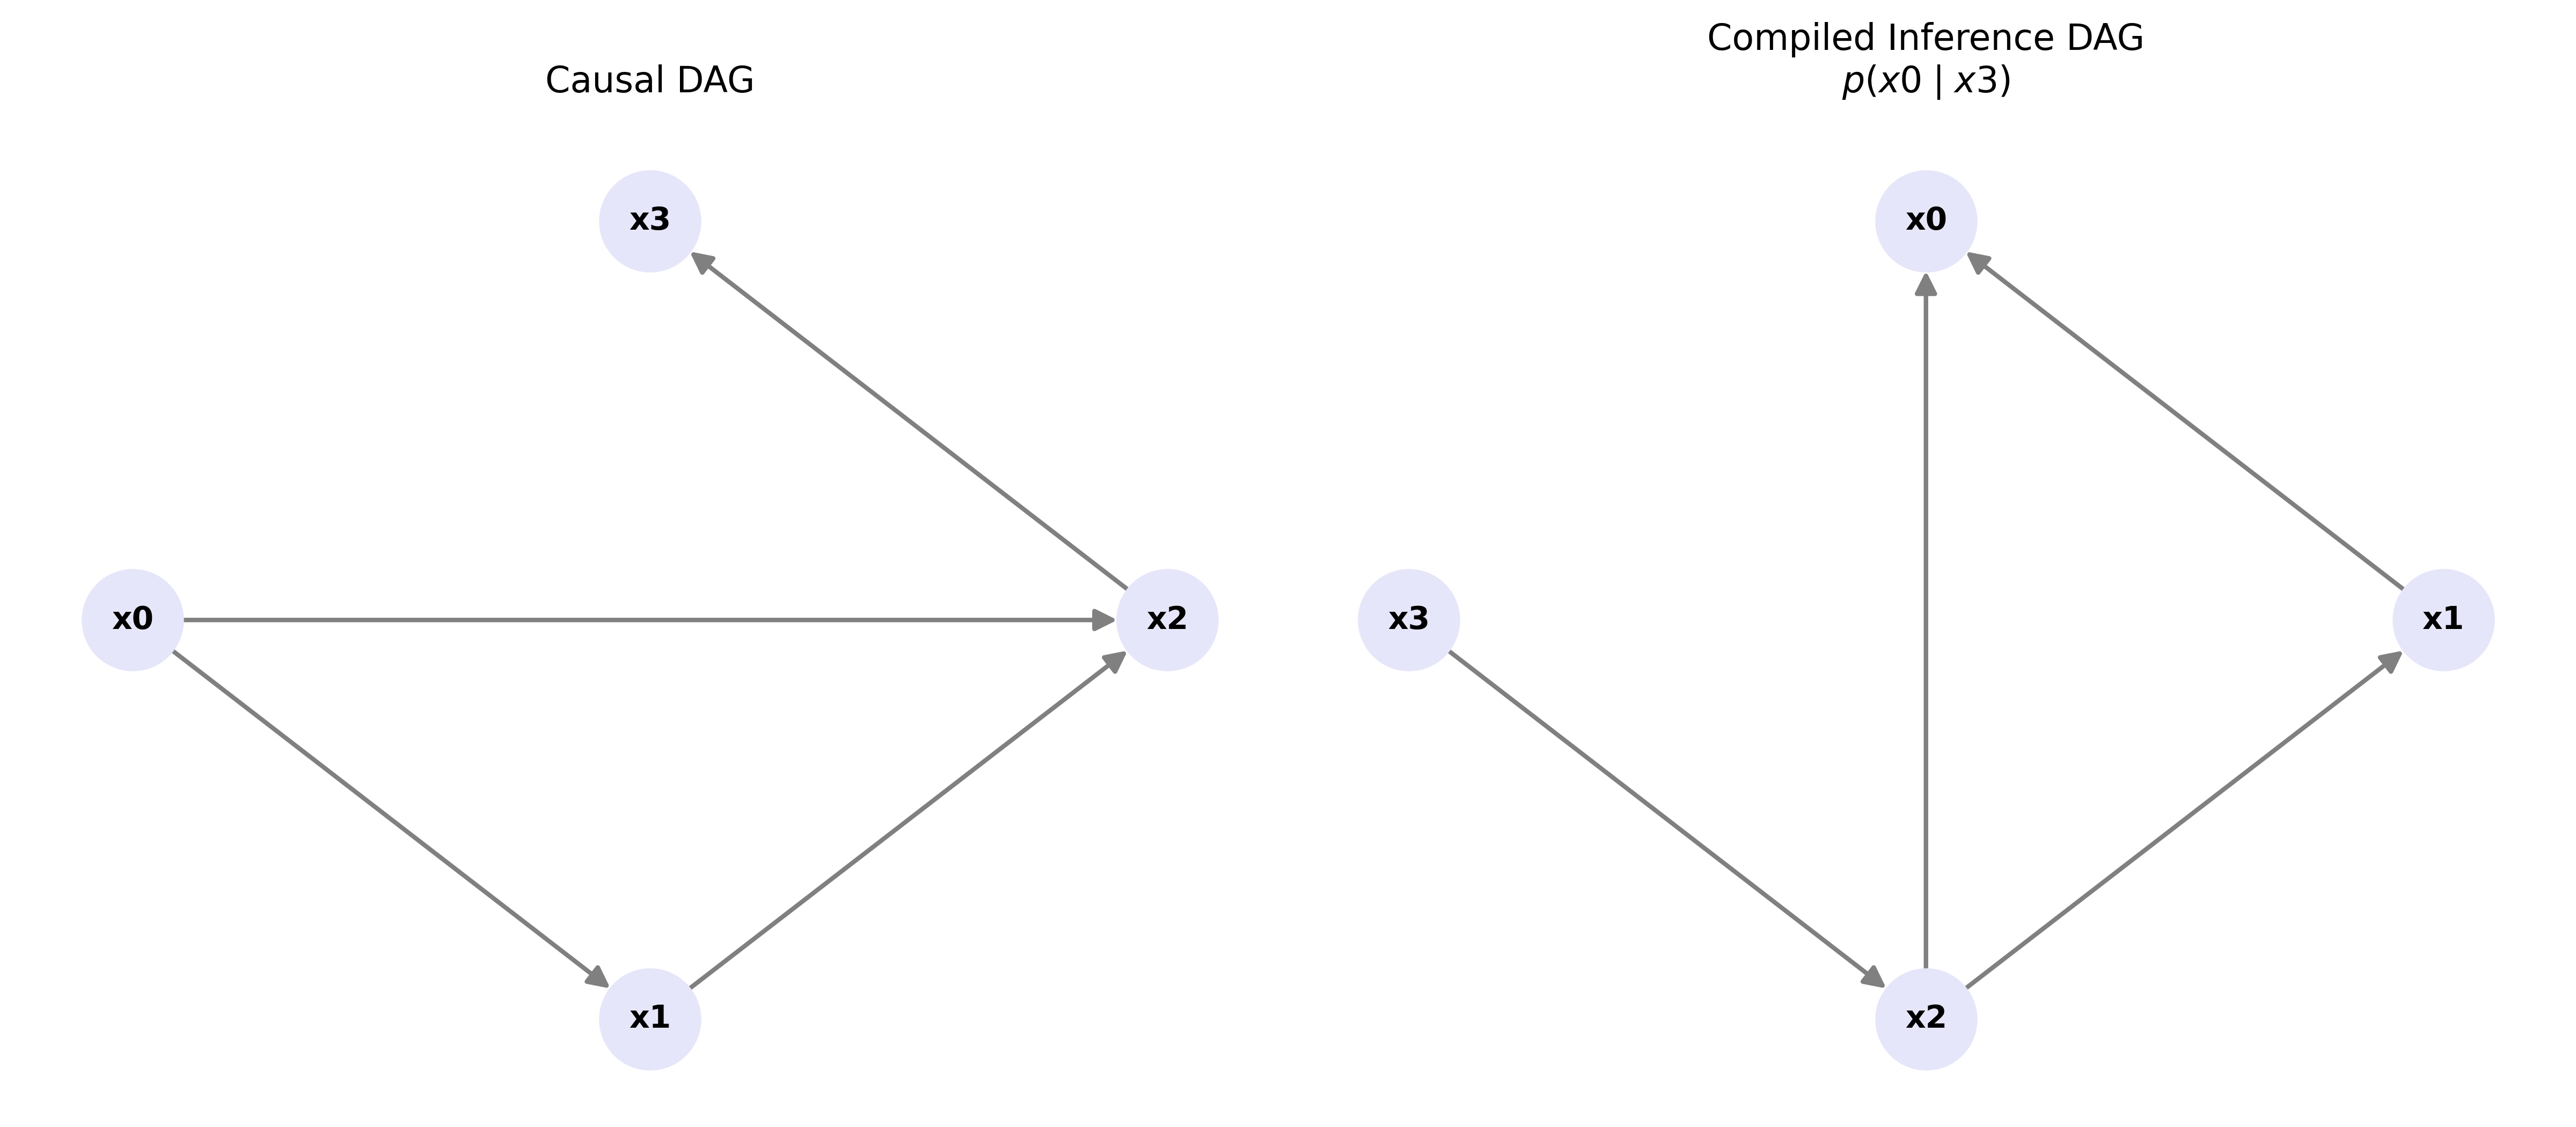
\includegraphics[width=0.68\columnwidth]{images/pgm_compilation_visualization_41_4.png}
    \caption{An example of StructFlow ($n=4$, Seed 41). We start with the given structure / DAG (left), which defines the dependencies of the causally-aligned flow. Alternatively, we compile the structure for inference (right), yielding a different DAG that supports inference queries.}
    \label{fig:example-pgm-compilation-41}
\end{figure}

\begin{figure}[hbt!]
    \centering
    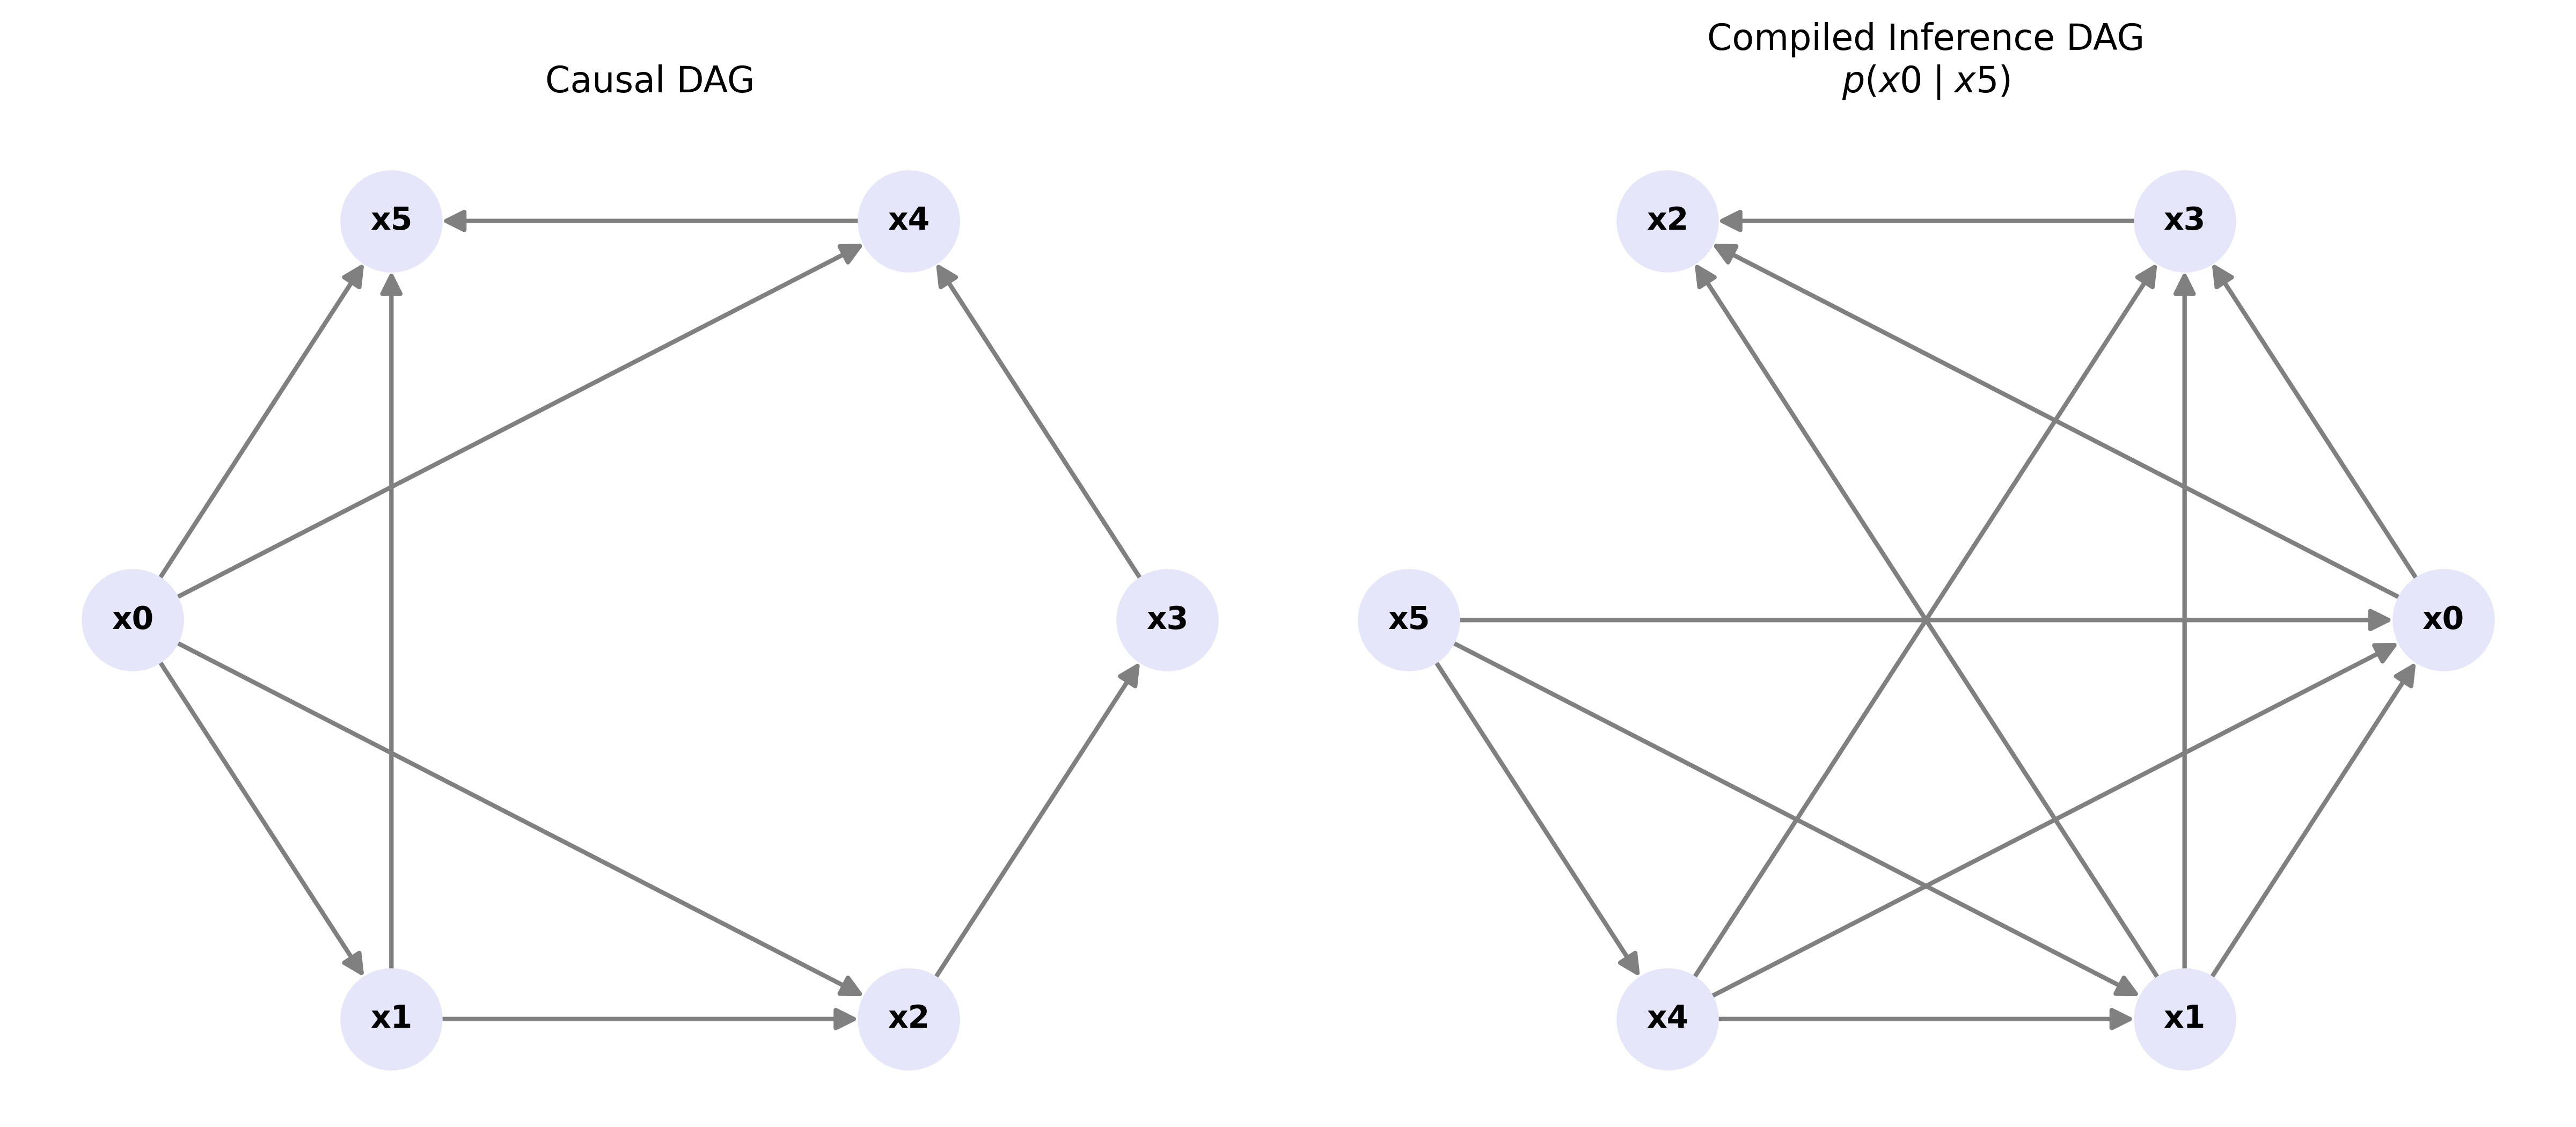
\includegraphics[width=0.68\columnwidth]{images/pgm_compilation_visualization_41_6.png}
    \caption{As Figure~\ref{fig:example-pgm-compilation-41}, for a denser graph ($n=6$, Seed 41).}
    \label{fig:example-pgm-compilation-41-6}
\end{figure}
\newpage
\section{Appendix: Architecture and Implementation}
\label{app:implementation}

In this section, we describe the neural network architecture and optimization techniques used to parameterize the block-triangular flows.

\subsection{Loss Function and Optimization}

For all models, we use the Adam optimizer \citep{Kingma2015} with a warmup-cosine decay learning rate schedule. This schedule provides an initial linear warmup period followed by a cosine annealing phase to ensure stable convergence.

The training objective for our one-sided flows follows the denoising-style loss for $\eta_1$-prediction:
\begin{equation}
    \mathcal{L}(\theta) = \mathbb{E}_{t \sim \mathcal{U}(0,1), y_1 \sim p_{data}, \epsilon \sim \mathcal{N}(0,I)} \left[ \| \hat{\eta}_1(y_t, t; \theta) - y_1 \|^2 \right]
\end{equation}
where $y_t = t y_1 + (1-t) \epsilon$ is the linear interpolant.

\subsubsection{Noise--Data Coupling}
\label{app:coupling}
\cam{Minibatch optimal transport (OT) couplings, which pair noise samples $\epsilon$ with data samples $y_1$ within each training batch, straighten flow trajectories \citep{tong2023conditional} and so reduce integration error. They preserve the \emph{joint} marginals, but a coupling computed on the full vector $y_1$ is not neutral for \emph{conditionals}: the noise paired with a block then depends on that block's conditions, so the population optimum of the flow-matching loss no longer transports to the correct conditional distributions \citep{cheng2025curse}. Which coupling is admissible therefore depends on the conditioning mode:
\begin{itemize}
    \item \textbf{Static:} independent pairing ($\epsilon \perp y_1$). Each block's network receives its conditions as clean inputs, and independent pairing is exact for every conditional.
    \item \textbf{Dynamic:} a per-block coupling in topological order. Each block's noise is matched to its data within the batch by a condition-aware OT plan \citep{cheng2025curse} whose cost adds the parents' squared distance with a weight chosen per batch by the adaptive rule of \citet{cheng2025curse}: the smallest weight for which at most $5\%$ of pairs $(i,j)$ have a combined cost below that of the unpermuted pair $(i,i)$. This is a minibatch Knothe--Rosenblatt coupling. Unlike independent pairing, this makes the marginal velocity of each block depend only on the block and its predecessors, which a block-triangular field can represent (Remark~\ref{rem:dynamic-consistency}).
    \item \textbf{Guided:} exact minibatch OT (Hungarian) on the joint vector; the guided flow models the joint, which this coupling preserves.
\end{itemize}

\paragraph{Population limit of the minibatch coupling on chains.} A batch-$128$ matching only approximates the Knothe--Rosenblatt coupling, so even at the optimum it leaves some bias. For the linear-Gaussian chains of Section~\ref{sec:chain-stiffness} this residual can be computed without training. We apply the training coupling to $300$ batches of $128$ standardized samples and take the empirical cross-covariance $C = \mathrm{Cov}(\epsilon, y_1)$. Treating $(\epsilon, y_1)$ as jointly Gaussian with that covariance, the best block-triangular field is linear: row $k$ is the regression of $\dot y^{(k)} = y_1^{(k)} - \epsilon^{(k)}$ on $y_t^{(1:k)}$. We integrate the induced covariance ODE from $\mathcal{N}(0, I)$ and compare $p(x_0 \mid x_{n-1})$ with the exact posterior in $W_2$. With the exact Knothe--Rosenblatt coupling (Cholesky) this gives $0$, and with independent pairing it matches the trained dynamic models to within $0.11$ at every depth. With the minibatch coupling it gives $0.009$, $0.012$, $0.028$, $0.053$ and $0.075$ for $n = 2, \dots, 32$. Each block's matched noise has correlation ${\approx}0.65$ with its exact Knothe--Rosenblatt noise at every depth: the per-block approximation does not degrade with depth, but its residual accumulates along the chain.}

\subsection{Neural Network Architecture}

For each variable in the PGM, we use a conditional block which computes the output (the velocity, or the prediction $\hat\eta_1$ of the clean data) of that variable given its current state $y_t$, the time $t$, and the values of its parent variables $\{p_i\}$ in the dependency graph.

\subsubsection{Residual Block Architecture}
Across all our conditional blocks and networks, we employ a consistent architecture based on residual layers. The key design is:
\begin{itemize}
    \item \textbf{Time Embedding:} The scalar time $t$ is embedded into a high-dimensional vector using Fourier features (random Gaussian projection followed by sin/cos transformations).
    \item \textbf{Input Projection:} The concatenated input (local state, time embedding, and parent states) is projected to a hidden dimension.
    \item \textbf{Residual Stack:} A stack of 8 residual layers, where each layer computes $h \gets h + \sigma(\text{Linear}(\text{LayerNorm}(h)))$. We use Layer Normalization \citep{Ba2016} and the Swish (SiLU) activation function \citep{Ramachandran2017, Elfwing2018} consistently throughout.
    \item \textbf{Output Projection:} A final linear layer projects the hidden representation to the target dimension.
\end{itemize}
This modular residual design is used consistently across all network variants (static conditioning, guidance, CAREFL conditioning, and parallel flows).

To further ensure comparability of the varying architectures (e.g., a single large joint flow versus many small conditional blocks), we adopt a parameter-budgeting approach. For a given budget (e.g., 100,000 parameters), we perform a search over the hidden width $W$ such that the total number of trainable weights in the architecture most closely matches the budget.

\subsection{Structured Flows}

We verify that our models have the intended structure; an example is shown in Figure~\ref{fig:extraction-visualization}.

\begin{figure}[hbt!]
    \centering
    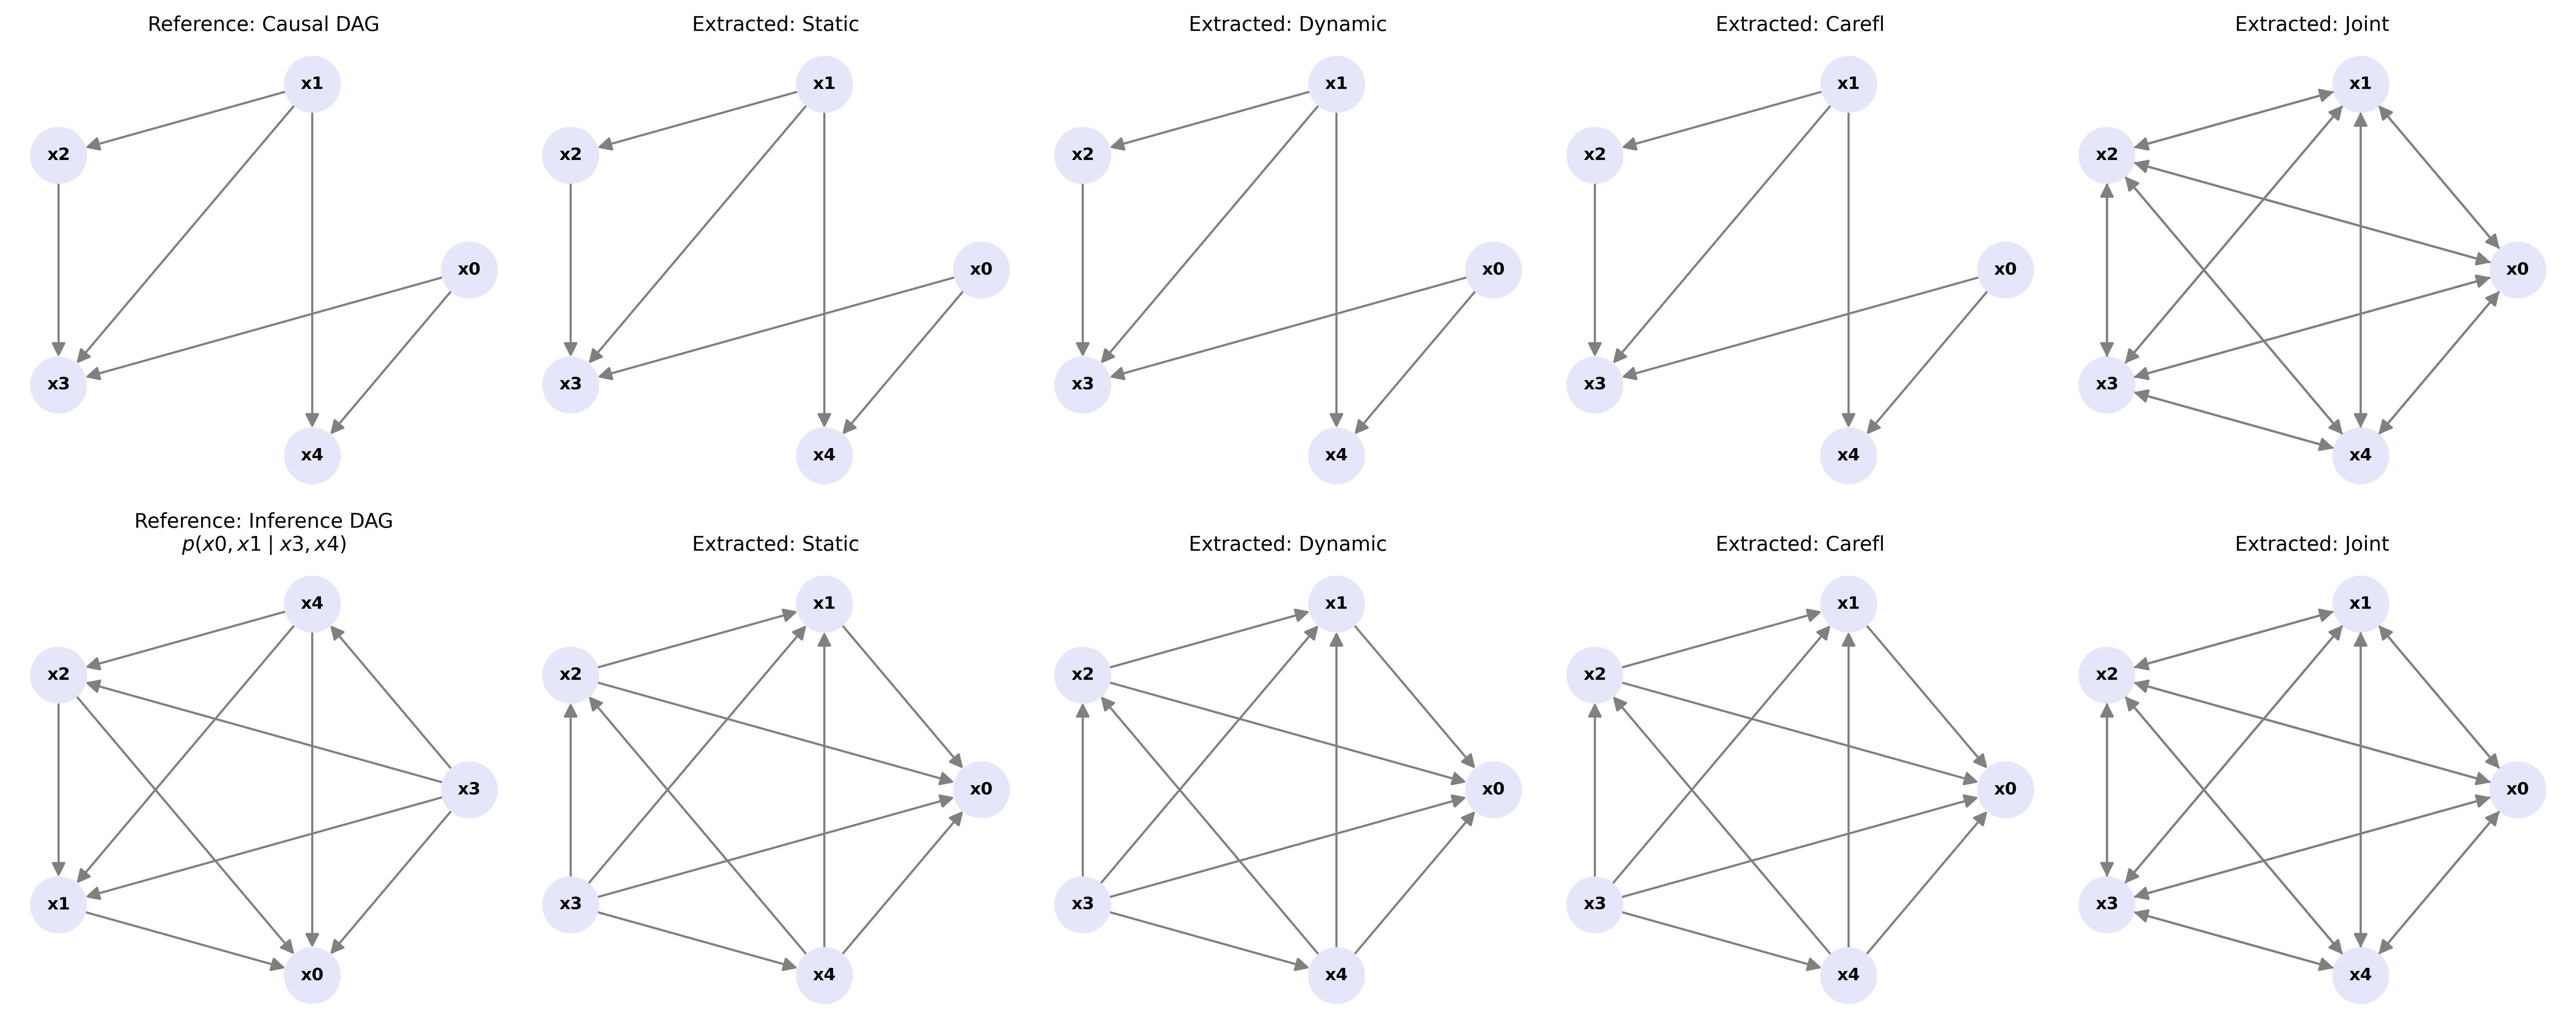
\includegraphics[width=\columnwidth]{images/pgm_compilation_and_extraction_visualization_42.png}
    \caption{Given a PGM, we extract its DAG. The DAG is either used directly as the structure of a causal flow, or compiled into an inference-aligned DAG from which an inference flow is built.}
    \label{fig:extraction-visualization}
\end{figure}

\newpage
\section{Appendix: Algorithms for Sampling and Inference}
\label{app:algorithms}

In this section, we provide the detailed algorithms for sampling and inference using our Structured Flow Matching framework. We distinguish between two conditioning paradigms: \texttt{Static} (for sequential sampling) and \texttt{Dynamic} (for parallel sampling); Figure~\ref{fig:static-v-dynamic-conditioning} contrasts the two schematically.

\begin{figure}[H]
    \centering
    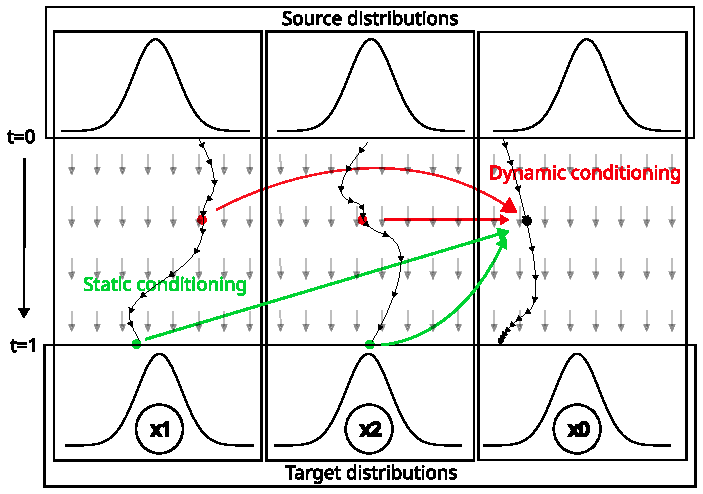
\includegraphics[width=0.72\textwidth]{images/collider-pgm-structured.pdf}
    \caption{\textbf{Static vs.\ Dynamic Conditioning.} Sampling $p(x_0 \mid x_1, x_2)$ with a block-triangular flow ordered $[x_1, x_2, x_0]$ (e.g.\ compiled from the collider $X_1 \to X_0 \leftarrow X_2$). Static conditioning (green) first integrates the conditioning blocks to completion and provides their final values $x_1^{(t=1)}, x_2^{(t=1)}$ as fixed inputs to the velocity field of $x_0$. Dynamic conditioning (red) integrates all blocks jointly in a single ODE solve, with $x_0$'s velocity conditioned on the evolving trajectories $x_1^{(t)}, x_2^{(t)}$ at each time step.}
    \label{fig:static-v-dynamic-conditioning}
\end{figure}

\subsection{Static Conditioning}

\subsubsection{Static Sampling}

In the Static mode, variables are sampled sequentially following a topological ordering of the dependency graph. Each variable's flow is conditioned on the \textit{final} values ($t=1$) of its parents. This minimizes the number of variables in any single ODE solve but requires $K$ separate integration passes for $K$ target variables.

\begin{algorithm}[H]
\caption{Static Conditional Sampling}
\label{alg:static_sampling}
\begin{algorithmic}
\REQUIRE Trained Velocity Field $v_\phi$, Observations $c$, Target variables $\Theta$
\ENSURE Samples $\theta_{t=1}$
\STATE $Order \gets \text{TopoSort}(\Theta \text{ with respect to } \text{Parents}(\Theta))$
\STATE $Context \gets c$ (Initial static conditions)
\FOR{$y \in Order$}
    \STATE Sample noise $z_y \sim \mathcal{N}(0, I)$
    \STATE Define single-block ODE: $\frac{dy}{dt} = v_\phi^{(y)}(t, y, Context)$
    \STATE Integrate $t: 0 \to 1$ starting from $y(0) = z_y$
    \STATE $Context[y] \gets y(1)$ (Update context for downstream blocks)
    \ENDFOR
    \STATE \textbf{return} $Context[\Theta]$
    \end{algorithmic}
\end{algorithm}

\subsubsection{Static Density Evaluation}

For static conditioning, the conditional log-probability $\log p(y_{targets} | y_{conditions})$ is computed by integrating the flow ODE backward from $t=1$ to $t=0$. By Proposition~\ref{prop:cond-density}, we compute the log-density by accumulating the divergence of the target variables only. Because the flow has a block-triangular Jacobian, the log-determinant term decomposes into a sum over individual blocks, allowing us to ignore the divergence of the conditioning variables.

\subsection{Dynamic Conditioning}

\subsubsection{Dynamic Sampling}

In the Dynamic mode, all variables are integrated simultaneously in a single monolithic ODE solve. This requires reproducing the full temporal trajectories ($t \in [0, 1]$) of the conditioning variables. While this approach requires a more complex trajectory-interpolation step, it allows the sampling process to be parallelized across blocks, which is advantageous for deep or highly connected graphs.

\begin{algorithm}[H]
\caption{Dynamic Conditional Sampling}
\label{alg:dynamic_sampling}
\begin{algorithmic}
\REQUIRE Trained Velocity Field $v_\phi$, Observations $c$, Target variables $\Theta$
\ENSURE Samples $\theta_{pred}$
\STATE $\mathcal{B} \gets \text{AllBlocks}()$ (All variable blocks in the model)
\STATE $\mathcal{C} \gets \text{Keys}(c)$ (Condition blocks from observations)
\STATE $\mathcal{S} \gets \text{RequiredSimulationBlocks}(\Theta, \mathcal{C})$ (Ancestors of $\Theta$ not in $\mathcal{C}$)
\STATE $z_{dict} \gets \{\}$
\IF{conditions $c$ provided}
    \STATE Construct $x^{(1)}_{cond}$ with observed values $c[\mathcal{C}]$ and zeros elsewhere
    \STATE Integrate backward $t: 1 \to 0$: $\frac{dx}{dt} = v_\phi(t, x)$ from $x(1) = x^{(1)}_{cond}$
    \STATE Extract $z_{cond} \gets z(0)$ for condition blocks only
    \STATE $z_{dict} \gets z_{cond}$
\ENDIF
\STATE $\text{ToSample} \gets \{b \in \mathcal{S} : b \notin z_{dict}\}$ (Blocks needing fresh noise samples)
\FOR{$b \in \text{ToSample}$}
    \STATE Sample $z_b \sim \mathcal{N}(0, I)$
    \STATE $z_{dict}[b] \gets z_b$
\ENDFOR
\STATE Fill remaining blocks: For $b \in \mathcal{B} \setminus z_{dict}$, sample or set to zero
\STATE Construct $x^{(0)} \gets \text{Flatten}(z_{dict})$ (Concatenate all noise blocks in order)
\STATE Integrate forward $t: 0 \to 1$: $\frac{dx}{dt} = v_\phi(t, x)$ from $x(0) = x^{(0)}$
\STATE $x^{(1)} \gets x(1)$
\STATE \textbf{return} $\text{Unflatten}(x^{(1)})[\Theta]$ (Extract target variables)
\end{algorithmic}
\end{algorithm}

The zero padding is allowed as parents are not dependent on children, and the conditions are guaranteed to be parents. Therefore, the zero padding has no effect on the backward simulation of the conditions.

\subsubsection{Dynamic Density Evaluation}

In the Dynamic (parallel) mode, density evaluation requires reconstructing the full temporal trajectories of the conditioning variables. We first integrate the full system (targets + conditions) backward from $t=1$ to $t=0$ to obtain the trajectories $\tau_{all}(t)$. We then define a subset velocity field $v_T(y_T, t; \tau_C)$ where the conditioning variables are interpolated from their backward trajectories. By Proposition~\ref{prop:cond-density}, we compute the log-density by accumulating the divergence of the target variables only, properly accounting for the dynamic coupling between variables without integrating the full joint density.
\newpage
\section{Appendix: Theoretical Proofs}
\label{app:proof}

\subsection{Proof of Theorem 1 (Asymmetry of Marginalization)}

\rev{\textbf{Theorem 1.} \textit{In a Block-Triangular Flow ordered $z_1 \to \dots \to z_K$, if $S$ is ancestrally closed (contains all parents, and hence all ancestors, of each of its members), the marginal log-density $\log p(z_S)$ is \emph{directly tractable}---evaluable by the change-of-variables formula restricted to $S$, in a single pass and with no integration over the remaining variables. Conversely, if $S$ is not ancestrally closed, the restricted formula is not valid in general: for any flow in which some missing ancestor's influence is functionally non-degenerate, exact evaluation requires integrating that ancestor out. A topological prefix is the canonical ancestrally-closed set.}}

\begin{proof}
Let the variables $z$ be partitioned into $K$ blocks, ordered topologically. The flow transformation $\Phi: z(0) \to z(1)$ is defined by the ODE $\frac{dz}{dt} = v_t(z)$.

\paragraph{1. Forward Direction (Ancestrally Closed is Tractable)}
Let $S$ be ancestrally closed. Due to the block-triangular structure, the velocity of any block $i \in S$ depends only on $i$ and its parents, all of which lie in $S$:
\begin{equation}
    v^{(i)}(z, t) = f\bigl(\{z^{(j)} : j \in \{i\} \cup \mathrm{Pa}(i)\}, t\bigr), \qquad \{i\}\cup\mathrm{Pa}(i) \subseteq S.
\end{equation}
Consequently, the time-evolution of $z_S$ is entirely self-contained; its trajectories do not depend on the variables outside $S$. We can treat $z_S$ as a standalone flow system, and the marginal log-density is given by the change of variables formula restricted to $S$:
\begin{equation}
    \log p(z_S(1)) = \log p(z_S(0)) - \int_0^1 \sum_{i \in S} \text{Tr}\left(\frac{\partial v^{(i)}}{\partial z^{(i)}}\right) dt
\end{equation}
Since all terms in the divergence sum are computable using only variables in $S$, the marginal density can be evaluated in a single pass without integration over the remaining variables. A prefix $S=\{1,\dots,k\}$ is a special case.

\paragraph{2. Reverse Direction (Not Ancestrally Closed)}
Suppose some block $j \in S$ has a parent $i \notin S$, and write $\bar S$ for the complement. The joint factorizes as $p(z_S, z_{\bar S}) = p(z_S \mid z_{\bar S})\,p(z_{\bar S})$, and the marginal requires integrating out $\bar S$:
\begin{equation}
    p(z_S) = \int p(z_S | z_{\bar S}) \, p(z_{\bar S}) \, d z_{\bar S}.
\end{equation}
In a non-linear flow the conditional $p(z_S | z_{\bar S})$ is a nonlinear function of $z_{\bar S}$ with no closed-form integral; a Monte Carlo estimate would re-sample $z_{\bar S}$, re-incurring the cost of the full joint model. Hence the marginal is not directly tractable and is intractable in general. \rev{Two scope remarks. First, the converse requires \emph{functional non-degeneracy}: if the architectural edge $i \to j$ happens to carry no actual dependence (the trained velocity is constant in $z^{(i)}$), the restricted formula can be accidentally valid; the theorem therefore claims invalidity for flows whose dependencies are functionally non-degenerate, which is the generic case and the intended reading of the architecture. Second, we claim intractability of \emph{exact, integration-free} evaluation, not a worst-case complexity lower bound.}
\end{proof}

\rev{\begin{corollary}[Supported query family]
\label{cor:query-family}
Let a compilation have block order $\mathcal{O} = (z_1, \dots, z_K)$ over \emph{all} graph variables, and let $C, T$ be disjoint subsets with $C = \{z_1, \dots, z_m\}$ a prefix of $\mathcal{O}$. Then:
(i) \textbf{(Sampling)} the compiled flow draws exact samples from its conditional $p(T \mid C{=}c)$ by clamping the prefix and integrating the remaining blocks in order, discarding draws of the nuisance set $N = V \setminus (C \cup T)$; this marginalizes $N$ by sampling, at the cost of only their block solves, and any nuisance block ordered after every target block is never integrated at all.
(ii) \textbf{(Density)} $p(T \mid C{=}c) = p(C \cup T)/p(C)$ is directly tractable whenever $C \cup T$ is ancestrally closed in the compiled graph (the prefix $p(C)$ always is); otherwise it falls under the converse of Theorem~1.
Queries whose condition set is \emph{not} a prefix of $\mathcal{O}$ are answered by compiling (and training) for a different ordering.
\end{corollary}

\begin{proof}
(i) By Proposition~1 the model factorizes autoregressively along $\mathcal{O}$, so clamping the prefix to $c$ and ancestrally sampling the remaining blocks draws from $p(V \setminus C \mid C{=}c)$; restricting attention to the $T$-coordinates of each draw is exact marginalization of $N$. Blocks ordered after every target need not be integrated because no target block's dynamics depend on them (they are successors in the compiled order). (ii) Both numerator and denominator are directly tractable by Theorem~1, the former by assumption, the latter because a prefix is ancestrally closed.
\end{proof}}

\subsection{Proof of Proposition 1 (Structural Preservation)}

\rev{\textbf{Proposition 1.} \textit{Assume velocity fields regular enough for unique, continuously differentiable flows (existence--uniqueness and spatial Lipschitzness; Assumptions~1--2 of \citet{jeong_conditional_2025}). (i)~If the denoiser model $\hat{\eta}_1(y, t)$ respects a block-triangular dependency graph, the induced velocity field $v_t(y)$ and flow map respect the same block-triangular dependency graph, and the learned density factorizes autoregressively along the ordering. (ii)~If block $k$ of the denoiser depends only on its graph parents, then under joint integration block $k$ of the flow map depends only on the base noise of $\{k\} \cup \mathrm{Anc}(k)$, and $p(y) = \prod_k p(y^{(k)} \mid y^{(\mathrm{Anc}(k))})$. (iii)~If blocks are integrated sequentially with parents resolved to their final values, $p(y) = \prod_k p(y^{(k)} \mid y^{(\mathrm{Pa}(k))})$, the Markov factorization of $\mathcal{G}$.}}

\begin{proof}
Let the state $y$ be partitioned into blocks $y^{(1)}, \dots, y^{(K)}$. By definition, a function is block-triangular if the $k$-th block outcome depends only on the prefix $y^{(1:k)} = [y^{(1)}, \dots, y^{(k)}]$.

\begin{enumerate}
    \item \textbf{Assumption:} Our neural network $\hat{\eta}_1$ is structured such that:
    \begin{equation}
        \hat{\eta}_1^{(k)}(y, t) = \text{NN}^{(k)}(y^{(1)}, \dots, y^{(k)}, t)
    \end{equation}

    \item \textbf{Affine Property:} For the linear interpolant used in this work ($y_t = (1-t)y_0 + ty_1$), the velocity field $v_t(y)$ is an affine combination of the input $y$ and the denoiser $\hat{\eta}_1$:
    \begin{equation}
        v_t(y) = \frac{\hat{\eta}_1(y, t) - y}{1 - t}
    \end{equation}
    This can be written more generally as $v_t(y) = c_1(t)y + c_2(t)\hat{\eta}_1(y, t)$. (The explicit $1/(1-t)$ form is singular at $t=1$, but the argument below uses only the affine-in-$\bigl(y,\hat{\eta}_1\bigr)$ structure, i.e.\ the coefficients $c_1, c_2$, which is the well-defined form; the block-triangularity conclusion does not depend on the value at the endpoint.)

    \item \textbf{Preservation:} The $k$-th block of the velocity field is:
    \begin{equation}
        v_t^{(k)}(y, t) = c_1(t)y^{(k)} + c_2(t)\hat{\eta}_1^{(k)}(y^{(1:k)}, t)
    \end{equation}
    Since $\hat{\eta}_1^{(k)}$ only depends on the prefix $y^{(1:k)}$, and the term $y^{(k)}$ is itself part of that prefix, it follows that $v_t^{(k)}$ depends strictly on $y^{(1:k)}$.
\end{enumerate}

Thus, the block-triangularity of the denoiser implies the block-triangularity of the velocity field. \rev{The flow map inherits it: for any prefix $y^{(1:k)}$, the subsystem $\dot{y}^{(1:k)} = v_t^{(1:k)}(y^{(1:k)})$ is autonomous in its own coordinates, and by existence--uniqueness its solution map is a well-defined function of the prefix of the initial condition alone. Sampling blocks in order therefore realizes an autoregressive factorization $p(y) = \prod_k p(y^{(k)} \mid y^{(1:k-1)})$, proving (i). Note that (i) alone establishes \emph{generic triangularity} with respect to the chosen ordering; the DAG-specific sparsity is the content of (ii) and (iii).

\paragraph{(ii) Parent-masked velocity, joint integration: ancestral sparsity.}
Suppose $v_t^{(k)}$ reads only $(y^{(\mathrm{Pa}(k))}, y^{(k)}, t)$. Fix $k$ and let $A = \{k\} \cup \mathrm{Anc}(k)$. Every block in $A$ has its parents in $A$, so the subsystem $\dot{y}^{(A)} = v_t^{(A)}(y^{(A)})$ is autonomous; by uniqueness, $y^{(k)}(1)$ is a function of the initial noise $u^{(A)}$ only. This is the sharpest sparsity the \emph{jointly integrated} flow map admits: although the velocity reads only parent \emph{trajectories}, those trajectories carry the ancestors' noise, so the map---and hence the conditional $p(y^{(k)} \mid y^{(1:k-1)})$---depends on ancestors in general, not parents alone. The factorization refines as follows: $\mathrm{Anc}(k)$ is ancestrally closed, so the restricted flow on $A \setminus \{k\}$ is an invertible triangular map (part (i)); conditioning on the ancestor \emph{values} $y^{(\mathrm{Anc}(k))}$ therefore pins their noise $u^{(\mathrm{Anc}(k))}$ exactly, and $y^{(k)} = \phi^{(k)}(u^{(\mathrm{Anc}(k))}, u^{(k)})$ with $u^{(k)}$ independent of everything else. Any non-ancestor predecessor $y^{(j)}$ is a function of noises independent of $u^{(k)}$ given $u^{(\mathrm{Anc}(k))}$, so $y^{(k)} \perp y^{(j)} \mid y^{(\mathrm{Anc}(k))}$ and $p(y^{(k)} \mid y^{(1:k-1)}) = p(y^{(k)} \mid y^{(\mathrm{Anc}(k))})$.

\paragraph{(iii) Sequential integration with resolved parents: Markov factorization.}
In the sequential (static) sampler, block $k$ is integrated only after its parents have reached their final values, and its velocity reads the \emph{resolved} parent values: $\dot{y}^{(k)} = v_t^{(k)}(y^{(k)}, y^{(\mathrm{Pa}(k))}(1), t)$. The solution map is then a measurable function of $(y^{(\mathrm{Pa}(k))}(1), u^{(k)})$ alone, with $u^{(k)}$ independent of all other noise, so the sampling kernel of block $k$ given the entire prefix is a function of the parent values only: $p(y^{(k)} \mid y^{(1:k-1)}) = p(y^{(k)} \mid y^{(\mathrm{Pa}(k))})$. Multiplying over $k$ gives exactly the Markov factorization of $\mathcal{G}$. This sequential case is the sampler used by the causal-alignment mode, and is why its interventional semantics (clamping a block and integrating descendants) samples the mutilated graph exactly.}
\end{proof}

\begin{remark}[Consistency at the optimum vs.\ guarantees by construction]
\label{rem:dynamic-consistency}
Parts (ii)--(iii) concern what the architecture enforces for \emph{every} parameter setting. \cam{Consistency at the training optimum requires more. Under joint flow matching with independent (or joint-OT) pairing of noise and data, the population minimiser of the loss over block-triangular fields is the row-wise projection of the marginal velocity, $\hat v^{(k)}_t = \mathbb{E}[\dot y^{(k)} \mid y^{(1:k)}_t]$. This equals the marginal velocity only if $\mathbb{E}[\dot y^{(k)} \mid y_t] = \mathbb{E}[\dot y^{(k)} \mid y^{(1:k)}_t]$ for every block, i.e.\ if the velocity of a block carries no information about later blocks. When the blocks are dependent this generally fails: the flow-matching loss then has a strictly positive floor over the block-triangular class, and dynamic conditioning is biased at the optimum, already with two blocks. For a bivariate Gaussian with correlation $\rho = 0.9$ and condition $y = c$, the optimum gives $p(\theta \mid y{=}c) = \mathcal{N}(0.571c,\, 0.436)$ instead of $\mathcal{N}(0.9c,\, 0.19)$; a trained network with the architecture used here reaches the predicted value. The posterior-accuracy bound of \citet[Thm.~1]{jeong_conditional_2025} is stated in terms of the flow-matching error against the unconstrained marginal velocity; for a block-triangular field this error does not vanish in general, so the bound does not by itself imply consistency of dynamic conditioning. The remedy is in the coupling rather than the architecture: pairing noise and data block by block in topological order (a Knothe--Rosenblatt coupling, Proposition~\ref{prop:kr-coupling}) makes the marginal velocity block-triangular, and dynamic conditioning is then exact at the optimum. All dynamic models in this paper are trained with the minibatch version of this coupling (Appendix~\ref{app:coupling}).

Beyond the optimum, finite training adds a second error. The bound of \citet[Thm.~1]{jeong_conditional_2025} scales as $e^{2L}\varepsilon^2$, where $\varepsilon$ is the flow-matching error averaged over the \emph{training} path measure, which controls nothing off that measure, while the Gr\"onwall factor $e^{2L}$ compounds local error along the solve. Section~\ref{sec:chain-stiffness} studies how this behaves on deep chains.}
\end{remark}

\cam{\begin{proposition}[Per-block (Knothe--Rosenblatt) coupling]
\label{prop:kr-coupling}
Let blocks be ordered topologically and let the coupling of base noise $e$ and data $y_1$ be the Knothe--Rosenblatt map $y_1 = T(e)$, $T^{(k)}(e) = T_k(e^{(k)};\, y_1^{(1:k-1)})$, with each $T_k(\cdot\,; y_1^{(1:k-1)})$ the Brenier (optimal transport) map from $\mathcal{N}(0, I)$ to $p(y^{(k)} \mid y^{(1:k-1)})$. Under the linear interpolant $y_t = (1-t)e + tT(e)$, the marginal velocity $\mathbb{E}[\dot y \mid y_t]$ is block-triangular. Hence the population optimum of flow matching over block-triangular fields equals the marginal velocity, and dynamic conditioning on any prefix is exact at the optimum.
\end{proposition}
\begin{proof}[Proof sketch]
$M_t(e) = (1-t)e + tT(e)$ is block-triangular because $T$ is. Its $k$-th diagonal block is $(1-t)\,\mathrm{Id} + t\nabla_{e^{(k)}}\varphi_k$ with $\varphi_k$ convex, hence strictly monotone and invertible for $t<1$, so $e = M_t^{-1}(y_t)$ can be solved block by block in order: $e^{(k)}$ is a function of $y_t^{(1:k)}$. The velocity $\dot y = T(e) - e$ is therefore a deterministic function of $y_t$ whose $k$-th block depends only on $y_t^{(1:k)}$, so $\mathbb{E}[\dot y \mid y_t] = \dot y$ is block-triangular and coincides with its row-wise projection. Dynamic conditioning on a prefix $y^{(1:m)} = c$ recovers $e^{(1:m)} = (T^{(1:m)})^{-1}(c)$ by backward integration and draws $e^{(m+1:K)} \sim \mathcal{N}(0,I)$ independently, so $y^{(m+1:K)}_1 = T^{(m+1:K)}(e;\, c) \sim p(y^{(m+1:K)} \mid y^{(1:m)}{=}c)$.
\end{proof}
In practice the coupling is computed per minibatch (one optimal assignment per block, with the block's parents as the condition of a condition-aware OT cost; Appendix~\ref{app:coupling}), which approximates $T$; block $k$'s velocity then depends on its ancestors, which the masked network reaches up to its depth. We verified the proposition in closed form on Gaussian structures (two blocks, a three-node chain, two 2-D blocks; irreducible loss $0$ under the coupling, versus $0.03$--$0.32$ under independent or joint-OT pairing) and with trained networks, where the per-block coupling reduces the conditional error of dynamic conditioning to that of static conditioning.}

\subsection{Derivation of Conditional Log-Density}
\label{app:cond-density}

\textbf{Proposition 2.} \textit{For a Block-Triangular Flow in which the conditioning variables $Y$ precede the targets $\Theta$ in the ordering (so that, by the block-triangular structure, the velocity of $Y$ does not depend on $\Theta$), the conditional log-density $\log p(\Theta | Y)$ is computed by accumulating the divergence of the velocity field with respect to $\Theta$ only.}

\begin{proof}
Consider the joint system $z = [Y, \Theta]$ ordered such that $Y$ precedes $\Theta$. The flow is defined by the system of ODEs:
\begin{align}
    \frac{dY}{dt} &= v_Y(Y, t) \\
    \frac{d\Theta}{dt} &= v_\Theta(\Theta, Y, t)
\end{align}
To evaluate $\log p(\Theta(1) | Y(1))$, we condition on the observed trajectories of $Y(t)$ for $t \in [0,1]$.
The block-triangular structure is exactly the hypothesis doing the work here: because $Y$ precedes $\Theta$, the velocity $v_Y$ takes no $\Theta$ input, so $Y$'s trajectory is independent of $\Theta$. This holds for both conditioning paradigms---in static conditioning $Y$ is integrated to completion first, and in dynamic conditioning $Y$ co-evolves but its dynamics still do not see $\Theta$. We can therefore view the evolution of $\Theta$ not as a coupled part of a joint system, but as a \textbf{non-autonomous} system where $Y(t)$ acts as a time-dependent external forcing term:
\begin{equation}
    \frac{d\Theta}{dt} = \tilde{v}_t(\Theta) = v_\Theta(\Theta, Y(t), t)
\end{equation}
The Jacobian of this conditional transformation $\Phi_{Y}: \Theta(0) \to \Theta(1)$ is simply the sub-block of the full Jacobian corresponding to the target variables:
\begin{equation}
    J_{\Theta} = \frac{\partial \tilde{v}_t}{\partial \Theta} = \frac{\partial v_\Theta}{\partial \Theta}
\end{equation}
Applying the instantaneous change of variables formula to this subsystem yields:
\begin{equation}
    \log p(\Theta(1) | Y(1)) = \log p_0(\Theta(0)) - \int_0^1 \text{Tr}\left( \frac{\partial v_\Theta}{\partial \Theta}(\Theta(t), Y(t), t) \right) dt
\end{equation}
This confirms that the volume change (divergence) of the conditioning variables $Y$ does not need to be computed or integrated, significantly reducing the computational cost for high-dimensional conditioning.
\end{proof}

\begin{corollary}[Interventional densities are directly tractable]
\label{cor:interventional-density}
Let the flow be causally aligned to $\mathcal{G}$ and let $\mathrm{do}(x^{(I)} = a)$ be any hard
intervention. Then the log-density of the interventional distribution is available in a
\emph{single} pass, with no divergence contribution from the intervened blocks:
\begin{equation}
\label{eq:interventional-density}
    \log \hat p\bigl(x^{(-I)} \mid \mathrm{do}(x^{(I)}{=}a)\bigr)
    = \log p_0\bigl(u_{-I}\bigr)
      - \int_0^1 \sum_{k \notin I}
        \mathrm{Tr}\!\left(\frac{\partial v^{(k)}}{\partial x^{(k)}}\right) dt .
\end{equation}
\end{corollary}

\begin{proof}
Clamping the blocks in $I$ removes them from the dynamics and replaces them by a fixed
trajectory, which enters the velocity of the remaining blocks only through their parent
slots. The remaining system is therefore a non-autonomous block-triangular flow forced by a
prescribed external signal---exactly the hypothesis of Proposition~2 with the conditioning
set $Y$ taken to be the intervened set $I$. Applying Proposition~2 gives
\eqref{eq:interventional-density}.
\end{proof}

\begin{remark}[What this buys, and what it does not]
\label{rem:density-scope}
Corollary~\ref{cor:interventional-density} is why the interventional comparisons of
Section~\ref{sec:experiments} can be scored by exact KL on the linear--Gaussian PGMs rather
than by a sample-based proxy: the model gives the interventional \emph{distribution}, not
merely samples from it. The analogous statement fails for counterfactuals, and it is worth
being precise about why. In a deterministic SCM with a \emph{fully observed} factual, the
abduction step pins the exogenous noise down exactly, so $p(Y_{x'} \mid X{=}x, Y{=}y)$ is a
point mass and there is no density to evaluate. The counterfactual becomes a genuine
distribution only under \emph{partial} observation, where it is the pushforward under the
mutilated mechanism of the posterior $p(u \mid x_{\mathrm{obs}})$ over the unresolved noise.
Evaluating that density therefore requires a posterior over noise---an inference-direction
object. Counterfactual densities under partial observation are thus precisely the query for
which the two compiled artifacts of Section~\ref{sec:structflow} must be used together; we
note this as a concrete direction rather than a solved case.
\end{remark}

\subsection{Expressivity Gap: CAREFL vs.\ CNF}

\rev{\textbf{Proposition 3 (Expressivity Gap).} \textit{Let the true SCM be $Y = f(\mathrm{Pa}(Y), \epsilon)$ with $\epsilon$ drawn from CAREFL's base distribution (standard Gaussian or Laplace), $f$ continuously differentiable and strictly monotone in $\epsilon$, and $\frac{\partial^2 f}{\partial \epsilon^2} \neq 0$ on a set of $(\mathrm{Pa}, \epsilon)$-values of positive probability. Then: (i)~\emph{mechanism level}: the $L^2(p)$ mechanism error $\inf_{a,b} \mathbb{E}\bigl[(f(\mathrm{Pa}, \epsilon) - a(\mathrm{Pa})\epsilon - b(\mathrm{Pa}))^2\bigr]$ of any CAREFL model is bounded away from zero, uniformly in the capacity of the conditioner networks $a, b$; (ii)~\emph{distribution level}: CAREFL's conditionals $p(y \mid \mathrm{pa})$ lie in the location--scale family of its base, so if the true conditional lies outside that family on a positive-measure set of parent values, the conditional distributional error (in $W_2$ or total variation) is also bounded away from zero. In contrast, a CNF can achieve arbitrarily small error in both senses as the capacity of its velocity network increases.}}

\begin{proof}
CAREFL generates each node by an affine transformation of its own exogenous noise:
\begin{equation}
    Y = a(\mathrm{Pa}(Y)) \cdot \epsilon + b(\mathrm{Pa}(Y))
\end{equation}
where $a, b$ are arbitrary neural networks of the parent values. Crucially, this is not an artifact of using a single layer: \citet{khemakhem2021causal} show (their Appendix~C) that a composition of affine autoregressive flows under a fixed ordering is \emph{itself} an affine autoregressive flow, so stacking layers preserves this form. The map is therefore \textbf{strictly linear in $\epsilon$}:
\begin{equation}
    \frac{\partial^2 Y}{\partial \epsilon^2} = 0 \quad \text{for all } a, b
\end{equation}

\rev{(i) For each parent value $\mathrm{pa}$, the map $\epsilon \mapsto a(\mathrm{pa})\epsilon + b(\mathrm{pa})$ ranges over the two-dimensional space $\mathrm{span}\{\epsilon, 1\}$; the $L^2(p_\epsilon)$-optimal choice is the orthogonal projection of $f(\mathrm{pa}, \cdot)$ onto that span, and the squared residual is zero iff $f(\mathrm{pa}, \cdot)$ is affine in $\epsilon$. By hypothesis the residual is positive on a positive-probability set of parent values, so its expectation over $\mathrm{Pa}$ is a positive constant independent of the capacity of $a, b$---capacity only helps choose the per-$\mathrm{pa}$ coefficients, which are already optimal. (ii) An affine map of the base variable has conditional law $a(\mathrm{pa})\,\epsilon + b(\mathrm{pa})$, i.e.\ a location--scale transform of the base density; the achievable conditionals are exactly that family. If the true conditional is outside the family for a positive-measure set of $\mathrm{pa}$, its distance to the family (in $W_2$ or TV, both of which metrize the gap to a closed location--scale family on compact sets) is positive there, and the expected conditional error is bounded below by a positive constant.}

In contrast, Continuous Normalizing Flows (CNFs) parameterize the transformation as the solution to an ODE:
\begin{equation}
    Y = \phi_1(\epsilon) = \epsilon + \int_0^1 v_t(\phi_t(\epsilon), \mathrm{Pa}(Y), t) \, dt
\end{equation}
For the scalar exogenous noise of a structural equation, the flow of a Neural ODE realizes an arbitrary smooth \emph{monotone} map $\epsilon \mapsto Y$, which is precisely the class of invertible scalar mechanisms; more generally, Neural ODEs are universal approximators of homeomorphisms given dimension augmentation \citep{zhang2020approximationcapabilitiesneuralodes}. In either case the mechanism can be approximated to arbitrary precision, so the approximation error $\to 0$ as the capacity of $v_t$ increases.
\end{proof}

\begin{remark}[The gap holds for the full CAREFL model, not just one layer]
Because composing affine autoregressive flows under a fixed ordering yields another affine autoregressive flow \citep[Appendix~C]{khemakhem2021causal}, the identity $\partial^2 Y/\partial\epsilon^2 = 0$ holds for the entire stacked CAREFL model used in practice, not merely a single layer; the proposition is therefore not an artifact of restricting the baseline's depth. The companion fact that affine/additive flows are not universal density approximators is their Appendix~B. The CNF escapes this constraint while retaining the single-transform structural reading on which our abduction step for counterfactuals (Section~\ref{sec:counterfactuals}) relies.
\end{remark}
\subsection{Recovery of the Causal Hierarchy}
\label{app:hierarchy}

This section answers the question left open by Remark~\ref{rem:cf-identifiability}: under
what conditions does a causally-aligned StructFlow converge to the \emph{true}
interventional and counterfactual distributions, rather than merely to the true
observational joint? The answer separates into three claims of decreasing strength, and the
third is a negative result.

\subsubsection{Setup}

Let $\mathcal{G}$ be a DAG on blocks $x^{(1)},\dots,x^{(K)}$ listed in topological order,
$x^{(k)} \in \mathbb{R}^{d_k}$, with data generated by a structural causal model
\begin{equation}
\label{eq:scm}
  \mathcal{M}: \quad x^{(k)} = f_k\bigl(x^{(\mathrm{Pa}(k))},\, \epsilon_k\bigr),
  \qquad \epsilon_1,\dots,\epsilon_K \ \text{mutually independent},
\end{equation}
satisfying Assumption~\ref{ass:standard}(i)--(ii). Write $p$ for the induced
joint, $p_{\mathrm{do}(x^{(I)}=a)}$ for the law under a hard intervention on the index set
$I$, and $p_0 = \mathcal{N}(0, I_d)$ for the base measure, partitioned conformally as
$u = (u_1,\dots,u_K)$. A \emph{causally-aligned} StructFlow is the CNF of
Section~\ref{sec:block-triangular} whose $k$-th velocity block reads
$v^{(k)}_\phi\bigl(x^{(k)}_t, x^{(\mathrm{Pa}(k))}_t, t\bigr)$, with flow map $\phi_1$ and
induced law $\hat p = (\phi_1)_\# p_0$.

\subsubsection{The learned flow is itself an SCM}

Proposition~\ref{prop:structural-preservation} states that the flow \emph{map} is
block-triangular. The following strengthens this: block $k$ depends on its parents only
through their \emph{terminal} values, so the flow map is literally a set of structural
equations driven by independent noise. This is the $K$-block generalisation of Lemma~1 of
\citet{jeong_conditional_2025}, which treats the two-block case
$T(y_0,\theta_0) = (F(y_0), G(F(y_0),\theta_0))$.

\begin{lemma}[Mechanism factorisation]
\label{lem:mech}
Let $\phi_1$ be the flow map of a causally-aligned StructFlow whose velocity field satisfies
the conditions of Proposition~\ref{prop:structural-preservation} and is Lipschitz in space.
Then there exist maps $G_1,\dots,G_K$ such that, for $u \sim p_0$ and $\hat x = \phi_1(u)$,
\begin{equation}
\label{eq:learned-scm}
  \hat x^{(k)} = G_k\bigl(\hat x^{(\mathrm{Pa}(k))},\, u_k\bigr),
  \qquad k = 1,\dots,K,
\end{equation}
with $u_1,\dots,u_K$ mutually independent and each $G_k(\,\cdot\,, w)$ a diffeomorphism in
$w$ at fixed parent values. That is, \emph{the learned flow is an SCM on $\mathcal{G}$}, and
$G_k$ is the Knothe--Rosenblatt (KR) rearrangement pushing $\mathcal{N}(0,I_{d_k})$ onto
$\hat p\bigl(x^{(k)} \mid x^{(\mathrm{Pa}(k))}\bigr)$.
\end{lemma}

\begin{proof}
By induction on the topological order. For $k=1$, $\mathrm{Pa}(1)=\emptyset$ and
$dx^{(1)}_t/dt = v^{(1)}(x^{(1)}_t,t)$ is closed in $x^{(1)}$, so $\hat x^{(1)} = G_1(u_1)$
with $G_1$ the time-$1$ flow of $v^{(1)}$, a diffeomorphism by Picard--Lindel\"of and the
Lipschitz hypothesis.

Assume the claim for all $j<k$. By the induction hypothesis and block-triangularity, the
trajectory $\{x^{(\mathrm{Pa}(k))}_t\}_{t\in[0,1]}$ is a deterministic function of $u_{<k}$,
and---since each $G_j$ is invertible---equivalently a deterministic function of the terminal
values $\hat x^{(\mathrm{Pa}(k))}$. Conditionally on that trajectory,
\begin{equation}
  \frac{dx^{(k)}_t}{dt} \;=\; \tilde v_t\bigl(x^{(k)}_t\bigr)
  \;:=\; v^{(k)}\bigl(x^{(k)}_t, x^{(\mathrm{Pa}(k))}_t, t\bigr)
\end{equation}
is a non-autonomous ODE in $x^{(k)}$ alone, whose time-$1$ map is a diffeomorphism of
$\mathbb{R}^{d_k}$. Composing with the trajectory-to-terminal-value identification gives
\eqref{eq:learned-scm}. Independence of the $u_k$ is that of the base blocks, and uniqueness
of the KR rearrangement \citep{Rosenblatt1952, Knothe1957} under the fixed within-block
ordering identifies $G_k$ as stated.
\end{proof}

\begin{remark}[Static and dynamic conditioning induce the same mechanism]
\label{rem:static-dynamic-equal}
The proof shows that $G_k$ depends on the parent trajectory only through its endpoint,
because the trajectory is a bijective image of that endpoint. In the population limit,
static and dynamic conditioning therefore realise the \emph{same} structural mechanism. This
also justifies the backward-integration step in the Action stage of
Section~\ref{sec:counterfactuals}: realising $\mathrm{do}(x^{(k)} = a)$ in a dynamic flow
requires the trajectory $a_t = F^{(k)}_t\bigl((F^{(k)}_1)^{-1}(a)\bigr)$, since this is the
unique trajectory with endpoint $a$, and it is exactly what the downstream blocks were
trained to read. The empirical static/dynamic gap on counterfactuals
(Section~\ref{sec:experiments}) is thus an approximation and numerical-inversion effect, not
a difference in the target object.
\end{remark}

\subsubsection{Level 2: interventions are recovered from the joint}

\begin{theorem}[Interventional recovery]
\label{thm:level2}
Assume \eqref{eq:scm} with Assumption~\ref{ass:standard}(i)--(ii), let the
StructFlow be causally aligned to the true $\mathcal{G}$, and suppose $\hat p = p$. Then for
every index set $I$ and value $a$,
$\hat p_{\,\mathrm{do}(x^{(I)}=a)} = p_{\,\mathrm{do}(x^{(I)}=a)}$, where the left-hand side
is the law obtained by clamping the blocks in $I$ to $a$ and integrating the remaining blocks
as usual. \emph{No restriction on the functional form of the $f_k$ is required.}
\end{theorem}

\begin{proof}
Matching joints have matching conditionals, so for every $k$,
$\hat p\bigl(x^{(k)} \mid x^{(1:k-1)}\bigr) = p\bigl(x^{(k)} \mid x^{(1:k-1)}\bigr)
= p\bigl(x^{(k)} \mid x^{(\mathrm{Pa}(k))}\bigr)$ ($p$-a.e.), the last step by the local
Markov property. By Lemma~\ref{lem:mech}, block $k$'s mechanism $G_k$ reads only
$x^{(\mathrm{Pa}(k))}$, so the two agree as \emph{mechanisms}, not merely as conditionals.
Clamping the blocks in $I$ leaves every other $G_k$ unchanged---possible precisely because
$\mathrm{Pa}(k) \subseteq \{1,\dots,k-1\}$ means no non-clamped block reads a clamped block
except through its parent slot---so the sampled law is
\begin{equation}
  \hat p_{\,\mathrm{do}(x^{(I)}=a)}(x) = \prod_{k \notin I}
  \hat p\bigl(x^{(k)} \mid x^{(\mathrm{Pa}(k))}\bigr)\Big|_{x^{(I)}=a}
  = \prod_{k \notin I} p\bigl(x^{(k)} \mid x^{(\mathrm{Pa}(k))}\bigr)\Big|_{x^{(I)}=a},
\end{equation}
which is Pearl's truncated factorisation, i.e.\ $p_{\,\mathrm{do}(x^{(I)}=a)}$
\citep[Thm.~3.2.2]{Pearl2009}.
\end{proof}

Level~2 therefore needs no identifiability condition beyond a correct graph: it is a
corollary of observational consistency. Combined with \citet{jeong_conditional_2025} this
yields a large-sample statement.

\begin{corollary}[Consistency of interventional queries]
\label{cor:level2-consistency}
Under the regularity conditions of \citet[Assumptions 1--4]{jeong_conditional_2025}, a
causally-aligned StructFlow trained by flow matching on $N$ i.i.d.\ samples from $p$
\cam{(with static conditioning, or with dynamic conditioning trained under the per-block coupling of Proposition~\ref{prop:kr-coupling}; otherwise the flow-matching loss of a block-triangular field has a positive floor, Remark~\ref{rem:dynamic-consistency})}
satisfies $\hat p_{\,\mathrm{do}(x^{(I)}=a)} \to p_{\,\mathrm{do}(x^{(I)}=a)}$ as
$N \to \infty$ for $p$-almost every $a$. Quantitatively, if the flow-matching loss is at most
$\varepsilon_N^2$ and each $f_k$ is $\ell$-Lipschitz in its parents,
\begin{equation}
\label{eq:overlap-bound}
  \mathbb{E}\Bigl[\,W_2^2\bigl(\hat p_{\,\mathrm{do}(x^{(I)}=A)},\,
  p_{\,\mathrm{do}(x^{(I)}=A)}\bigr)\Bigr]
  \;\le\; C\bigl(\ell, \mathrm{depth}(\mathcal{G})\bigr)\; \kappa_I \; \varepsilon_N^2 ,
\end{equation}
where $A \sim q$ for any distribution $q$ over intervention values and
$\kappa_I = \bigl\| \mathrm{d}q / \mathrm{d}p(x^{(I)}) \bigr\|_\infty$ is an overlap constant.
\end{corollary}

\begin{proof}[Proof sketch]
Theorem~2 of \citet{jeong_conditional_2025} gives $\varepsilon_N \to 0$ a.s.\ for ReLU MLP
velocity fields over a Sobolev ball; their Theorem~1 converts this into
$\mathbb{E}_{p}\bigl[W_2^2(\hat p(\cdot\mid Y), p(\cdot \mid Y))\bigr] \le
2Le^{2L}\varepsilon_N^2$ for a two-block split, with $L=\int_0^1 L_t\,dt$ the integrated
Lipschitz constant of the velocity. Applying that bound blockwise via Lemma~\ref{lem:mech}
and propagating along the topological order with the mechanism Lipschitz constant $\ell$
gives $C(\ell,\mathrm{depth})$, which grows like $\prod_k(1+\ell)$ along the longest directed
path: error compounds with graph \emph{depth}, not node count. The factor $\kappa_I$ appears
because the flow-matching loss controls error only in $p$-average over parent configurations,
whereas an intervention evaluates the mechanism at values drawn from $q$; the change of
measure costs a density ratio.
\end{proof}

\begin{remark}[The overlap constant is not removable]
\label{rem:overlap}
Equation~\eqref{eq:overlap-bound} is vacuous for intervention values outside the support of
$p(x^{(I)})$. This is not an artefact of the proof: an observationally-trained model has no
information about mechanism behaviour at parent configurations it never saw, and clamping is
exactly an out-of-distribution evaluation of the velocity field. This is the positivity /
overlap condition of classical causal inference reappearing, and it delimits the scope of any
claim that interventions come for free from observational data.
\end{remark}

\subsubsection{Level 3: counterfactuals under invertible mechanisms}

The counterfactual level is where functional form begins to matter. The key observation is
that for a broad class of mechanisms the KR rearrangement the flow is forced to learn
coincides with the true mechanism \emph{up to a reparameterisation of the noise that cancels
between abduction and prediction}.

\begin{theorem}[Counterfactual recovery]
\label{thm:level3}
Assume the setting of Theorem~\ref{thm:level2} ($\hat p = p$, correct $\mathcal{G}$), and in
addition that each mechanism satisfies one of:
\begin{enumerate}
  \item[(a)] \textbf{Scalar bijective:} $d_k = 1$, $\epsilon_k \in \mathbb{R}$ with continuous
  strictly increasing c.d.f.\ $F_{\epsilon_k}$, and $\varepsilon \mapsto
  f_k(\mathrm{pa}, \varepsilon)$ strictly increasing for every $\mathrm{pa}$; or
  \item[(b)] \textbf{Additive:} $f_k(\mathrm{pa}, \epsilon_k) = g_k(\mathrm{pa}) + \epsilon_k$
  with $\epsilon_k \in \mathbb{R}^{d_k}$ arbitrarily distributed.
\end{enumerate}
Then abduction--action--prediction (Section~\ref{sec:counterfactuals}) executed on the learned
flow returns \emph{exactly} the true counterfactual:
$\hat x_{\mathrm{cf}} = x_{\mathrm{cf}} =
\mathcal{M}_{\mathrm{do}(x^{(I)}=a)}\bigl(\epsilon(x_{\mathrm{obs}})\bigr)$.
Linear structural equations $x^{(k)} = B_k x^{(\mathrm{Pa}(k))} + \epsilon_k$ satisfy (b), and
when $d_k=1$ also (a); counterfactuals in linear SCMs---Gaussian or not---are therefore
recovered exactly.
\end{theorem}

\begin{proof}
\emph{Case (a).} Fix $k$ and parent values $\mathrm{pa}$. Strict monotonicity gives
$F_{x^{(k)}\mid \mathrm{pa}}\bigl(f_k(\mathrm{pa},\varepsilon)\bigr) = F_{\epsilon_k}(\varepsilon)$,
hence
\begin{equation}
\label{eq:reparam}
  f_k(\mathrm{pa}, \varepsilon)
  = F^{-1}_{x^{(k)}\mid \mathrm{pa}}\bigl(F_{\epsilon_k}(\varepsilon)\bigr)
  = G_k\bigl(\mathrm{pa},\, r_k(\varepsilon)\bigr),
  \qquad r_k := \Phi^{-1} \circ F_{\epsilon_k},
\end{equation}
where $G_k(\mathrm{pa}, w) = F^{-1}_{x^{(k)}\mid \mathrm{pa}}(\Phi(w))$ is the scalar KR map,
which by Lemma~\ref{lem:mech} and $\hat p = p$ is exactly the learned mechanism. Crucially
$r_k$ does not depend on $\mathrm{pa}$. Abduction in topological order therefore yields
$\hat u_k = G_k^{-1}\bigl(x^{(\mathrm{Pa}(k))}_{\mathrm{obs}},\,x^{(k)}_{\mathrm{obs}}\bigr)
= r_k(\epsilon_k)$: the true exogenous noise up to the fixed monotone reparameterisation
$r_k$. Prediction with counterfactual parents $\mathrm{pa}'$ (computed recursively, the base
case being the clamped blocks) gives
\begin{equation}
  \hat x^{(k)}_{\mathrm{cf}} = G_k(\mathrm{pa}', \hat u_k)
  = G_k\bigl(\mathrm{pa}', r_k(\epsilon_k)\bigr)
  = f_k(\mathrm{pa}', \epsilon_k) = x^{(k)}_{\mathrm{cf}},
\end{equation}
the reparameterisation cancelling. Induction over the topological order completes the case.

\emph{Case (b).} For additive noise the conditional law is
$p\bigl(x^{(k)} \mid \mathrm{pa}\bigr) = p_{\epsilon_k}\bigl(\cdot - g_k(\mathrm{pa})\bigr)$,
a pure translate of a fixed law. We claim its KR map is the corresponding translate of the KR
map $T_k$ of $p_{\epsilon_k}$, i.e.\ $G_k(\mathrm{pa}, w) = g_k(\mathrm{pa}) + T_k(w)$. For
the first within-block coordinate,
$F^{-1}_{x^{(k),1}\mid \mathrm{pa}}(\Phi(w^1)) = g_k^1(\mathrm{pa}) +
F^{-1}_{\epsilon_k^1}(\Phi(w^1))$. Inductively, conditioning on $x^{(k),1:j-1}$ is equivalent
to conditioning on $\epsilon_k^{1:j-1} = x^{(k),1:j-1} - g_k^{1:j-1}(\mathrm{pa})$, whose value
under the induction hypothesis is $T_k^{1:j-1}(w^{1:j-1})$ and is independent of
$\mathrm{pa}$; so coordinate $j$ is again a $\mathrm{pa}$-shift of a fixed conditional
quantile. Hence
\begin{equation}
  \hat u_k = T_k^{-1}\bigl(x^{(k)}_{\mathrm{obs}} - g_k(\mathrm{pa}_{\mathrm{obs}})\bigr)
           = T_k^{-1}(\epsilon_k),
  \qquad
  \hat x^{(k)}_{\mathrm{cf}} = g_k(\mathrm{pa}') + T_k(\hat u_k)
           = g_k(\mathrm{pa}') + \epsilon_k = x^{(k)}_{\mathrm{cf}} .
\end{equation}
\end{proof}

\begin{remark}[The linear case, explicitly]
\label{rem:linear-explicit}
For $x = Bx + \epsilon$ with $B$ strictly lower-triangular in topological order, the true
mechanism is $x^{(k)} = B_k x^{(\mathrm{Pa}(k))} + A_k u_k$ for \emph{any} square root
$A_kA_k^\top = \mathrm{Cov}(\epsilon_k)$, whereas KR uniqueness forces the flow to learn the
Cholesky factor $L_k$. The two noise assignments differ, yet the counterfactual is invariant:
\begin{equation}
  \hat x^{(k)}_{\mathrm{cf}}
  = B_k \mathrm{pa}' + L_k L_k^{-1}\bigl(x^{(k)}_{\mathrm{obs}} - B_k \mathrm{pa}_{\mathrm{obs}}\bigr)
  = B_k\bigl(\mathrm{pa}' - \mathrm{pa}_{\mathrm{obs}}\bigr) + x^{(k)}_{\mathrm{obs}},
\end{equation}
which is the true counterfactual and involves neither $A_k$ nor $L_k$. In the linear case the
only quantity that must be estimated correctly is the regression matrix $B$, which the joint
identifies given $\mathcal{G}$.
\end{remark}

\begin{remark}[Where Theorem~\ref{thm:level3} does not apply]
\label{rem:l3-limits}
Condition (a) is the bijective-SCM condition of \citet{nasresfahany2023bijective}; condition
(b) is the additive-noise condition. Both fail for a \emph{multivariate, non-additive} block,
where the true noise-to-value map need not be triangular in the within-block ordering and KR
uniqueness then selects a different---observationally indistinguishable---mechanism. The image
block of the Colored-MNIST model (Section~\ref{sec:colored-mnist}) is of this kind, so its
counterfactuals remain model-based estimates. Our scalar-node synthetic benchmarks
(Appendix~\ref{app:experiments}), whose mechanisms are invertible in a scalar noise by
construction, fall under case (a) and are covered by the theorem.
\end{remark}

\subsubsection{Level 0: the graph is the binding constraint}

All of the above is conditional on $\mathcal{G}$ being the true causal DAG, and that
assumption cannot be discharged from observational data in the linear--Gaussian case.

\begin{proposition}[Non-identifiability of the linear--Gaussian graph]
\label{prop:mec}
Let $p$ be generated by a linear--Gaussian SCM on $\mathcal{G}$. For every DAG $\mathcal{G}'$
in the Markov equivalence class of $\mathcal{G}$ there is a linear--Gaussian SCM on
$\mathcal{G}'$ inducing the same $p$. Consequently a StructFlow causally aligned to
$\mathcal{G}'$ attains the same optimal flow-matching loss as one aligned to $\mathcal{G}$,
while in general returning different---and incorrect---interventional and counterfactual
answers.
\end{proposition}

\begin{proof}
The first claim is standard \citep{Peters2017}: Markov-equivalent DAGs encode the same
conditional independencies, and any Gaussian distribution Markov to $\mathcal{G}'$ factorises
as a linear--Gaussian SCM on $\mathcal{G}'$ via successive regressions. Since the
flow-matching optimum depends on the architecture only through the family of joints it can
represent, and both aligned architectures represent $p$ exactly, both attain the same loss.
Concretely, for $X \to Y$ with $(X,Y)$ standard bivariate normal of correlation $\rho$, the
reversed model $Y \to X$ reproduces $p$ exactly but yields
$\hat p\bigl(y \mid \mathrm{do}(x)\bigr) = \mathcal{N}(0,1) \neq
\mathcal{N}\bigl(\rho x, 1-\rho^2\bigr) = p\bigl(y \mid \mathrm{do}(x)\bigr)$.
\end{proof}

Gaussianity is doing all the damage here, and dropping it repairs the chain.

\begin{corollary}[End-to-end recovery for linear non-Gaussian SCMs]
\label{cor:lingam}
Suppose the data are generated by a linear SCM $x = Bx + \epsilon$ with mutually independent,
non-Gaussian $\epsilon_k$ of finite variance (a LiNGAM model,
\citealp{shimizu2006lingam}). Then $\mathcal{G}$ and $B$ are identified from $p$ alone, and a
StructFlow aligned to the identified graph and fitted consistently recovers, in the
large-sample limit, the true observational, interventional \emph{and} counterfactual
distributions---all three levels of Pearl's hierarchy. The same holds for linear--Gaussian
SCMs with equal error variances \citep{peters2014identifiability} and for non-linear
additive-noise models with identifiable structure \citep{hoyer2008nonlinear}.
\end{corollary}

\begin{proof}
Identifiability of $(\mathcal{G}, B)$ is \citet{shimizu2006lingam}. Given the identified
$\mathcal{G}$, Theorem~\ref{thm:level2} and Corollary~\ref{cor:level2-consistency} give the
interventional claim, and Theorem~\ref{thm:level3}(b) the counterfactual claim, linear
mechanisms being additive.
\end{proof}

\begin{remark}[Summary, and the honest split verdict]
\label{rem:hierarchy-summary}
\emph{Given} the causal graph, a consistently trained causally-aligned StructFlow provably
reaches Level~2 for arbitrary mechanisms (Theorem~\ref{thm:level2}) and Level~3 for
scalar-bijective or additive mechanisms (Theorem~\ref{thm:level3}), linear problems being the
easiest instance of both. What a flow trained on observational data \emph{cannot} do is
discover the graph in the linear--Gaussian setting (Proposition~\ref{prop:mec}): there, the
very Gaussianity that makes the interventional and counterfactual algebra trivial makes the
causal direction invisible. Structure discovery is therefore not merely orthogonal to our
framework but is the \emph{sole remaining gap} between StructFlow's guarantees and a claim of
full causal identification.
\end{remark}

\subsection{Abduction Fidelity: Flow Inversion vs.\ DDIM Inversion}
\label{app:inversion}

Counterfactual reasoning at Level~3 requires \emph{inverting} the learned map (the Abduction
step). Theorem~\ref{thm:level3} concerns the exact map; in practice both a CNF and a
deterministic diffusion sampler realise it only approximately, and the two approximations
have different characters. Since diffusion-based causal models
\citep{sanchez2022diffusion, chao2023interventional} perform abduction by DDIM inversion,
this is the one place where the choice of backbone---rather than the choice of
structure---has a measurable consequence.

\begin{proposition}[Abduction error]
\label{prop:abduction-error}
Let $\phi_1$ be the flow map of a CNF and let $\hat\phi_1^{-1}$ denote numerical abduction.
\begin{enumerate}
  \item For a CNF, $\phi_1$ is \emph{defined} as the solution of an ODE. Forward and reverse
  passes integrate the same field $v_t$, so the reconstruction error
  $\|\hat\phi_1^{-1}(\phi_1(u)) - u\|$ is a pure ODE integration error: it is $O(h^{\,p})$
  for a $p$-th order scheme and is controllable to arbitrary tolerance by adaptive step-size
  control at fixed model weights.
  \item For a DDIM sampler at $N$ steps, the generative map is \emph{defined} by the discrete
  chain. Its standard inversion is not the algebraic inverse of that chain: it additionally
  assumes $\epsilon_\theta(x_t,t) \approx \epsilon_\theta(x_{t-1},t-1)$ across a step. The
  resulting reconstruction error therefore carries a first-order term in the step size that
  no tolerance parameter removes; it vanishes only as $N \to \infty$, which is precisely the
  limit in which the DDIM chain converges to the probability-flow ODE.
\end{enumerate}
\end{proposition}

\begin{remark}[Interpretation]
\label{rem:inversion-interp}
Proposition~\ref{prop:abduction-error} should not be read as ``diffusion models cannot do
counterfactuals''---they demonstrably can \citep{sanchez2022diffusion, chao2023interventional},
and we say so in Section~\ref{sec:experiments}. It should be read as a statement about
\emph{where the error budget goes}. Abduction fidelity is a solver-tolerance question for a
CNF and a step-count question for a DDIM sampler, and the step-count limit that removes the
DDIM bias is the limit in which the sampler becomes the continuous-time flow. This yields a
falsifiable prediction, which we test in Section~\ref{sec:backbone-ablation}: at matched
sampling compute (number of function evaluations), counterfactual accuracy should degrade
more sharply for a diffusion backbone than for a CNF backbone, while interventional accuracy
---which requires no inversion---should be comparable.
\end{remark}

\newpage
\section{Appendix: Experimental Setup}
\label{app:experiments}

\subsection{Benchmarks}
\label{sec:benchmarks}

We evaluate our framework on two classes of synthetic Probabilistic Graphical Models (PGMs): Linear Gaussian PGMs and Non-linear PGMs with neural mechanisms. These benchmarks allow us to verify the correctness of the PGM Compiler and the accuracy of the learned flows against ground-truth distributions.

\subsubsection{Linear Gaussian PGMs}
The Linear Gaussian PGM is defined by the following structural equation:
\begin{equation}
    x = Wx + b + S\epsilon
\end{equation}
where $x \in \mathbb{R}^D$ is a vector of $D$ variables, $W \in \mathbb{R}^{D \times D}$ is a strictly lower-triangular weight matrix representing the causal dependencies, $b \in \mathbb{R}^D$ is a bias vector, and $\epsilon \sim \mathcal{N}(0, I)$ is exogenous Gaussian noise. The matrix $S$ scales the noise for each variable.

In our experiments, we use random PGMs which we generate by sampling edges from a lower-triangular matrix with a specified sparsity $s$. Weights and biases are sampled from a standard normal distribution, and noise scales are sampled uniformly from $[0.1, 1.0]$.

The joint distribution of a Linear Gaussian PGM is a multivariate Gaussian $p(x) = \mathcal{N}(\mu, \Sigma)$, where:
\begin{equation}
    \mu = (I-W)^{-1}b, \quad \Sigma = (I-W)^{-1} SS^T (I-W)^{-T}
\end{equation}
This analytical form allows for exact computation of all marginal and conditional distributions for comparison.

\subsubsection{Non-linear Noise PGMs}
To test the framework's ability to handle complex, non-linear dependencies, we implement a class of PGMs where mechanisms are \textbf{nonlinear functions of both parents and noise}. For each node $i$, the mechanism is:
\begin{equation}
     x_i = f_i(\text{Pa}(x_i), \epsilon_i)
\end{equation}
where $f_i$ is an invertible transformation with respect to the noise $\epsilon_i \sim \mathcal{N}(0, 1)$. This design produces \textbf{truly non-Gaussian conditionals} $p(x_i | \text{Pa}(x_i))$, unlike standard non-linear PGMs where the conditional is necessarily Gaussian.

\paragraph{Mechanism Architecture:}
The mechanism $f_i$ is implemented as a \textbf{rational quadratic spline} transformation, conditioned on parent values. The spline parameters (widths, heights, and derivatives) are computed by a small neural network:
\begin{equation}
     \text{(widths, heights, derivatives)} = \text{MLP}_{\theta}(\text{Pa}(x_i))
\end{equation}
Each MLP consists of 2 hidden layers with a width of 32 units and uses \textbf{tanh} activation functions. The spline operates within a bounded domain $[-\text{bound}, \text{bound}]$ (typically $\text{bound} = 4.0$) with a configurable number of bins $K$ (typically $K = 8$). Outside the bounded domain, the spline behaves as the identity transformation.

\paragraph{Log-Probability Computation:}
Unlike standard non-linear PGMs where the conditional is always Gaussian, the true conditional distribution here is non-Gaussian. We compute log-probabilities using the change of variables formula:
\begin{equation}
     \log p(x_i | \text{Pa}(x_i)) = \log p(\epsilon_i) - \log \left| \frac{\partial f_i}{\partial \epsilon_i} \right|
\end{equation}
where $\epsilon_i = f_i^{-1}(x_i, \text{Pa}(x_i))$ is the recovered noise obtained by inverting the spline transformation. The invertibility of the rational quadratic spline ensures that both the forward transformation and its inverse can be computed efficiently with accurate log-determinant Jacobian tracking.

\paragraph{Inference and Ground Truth:}
The marginals and posteriors of these Non-linear Noise PGMs are not analytically tractable. To evaluate our flows, we use \textbf{No-U-Turn Sampling (NUTS)} via the \texttt{blackjax} library to generate high-fidelity ground-truth samples from the joint distribution. We use 1000 samples with 500 warmup steps for each evaluation query.

\begin{figure}[hbt!]
    \centering
    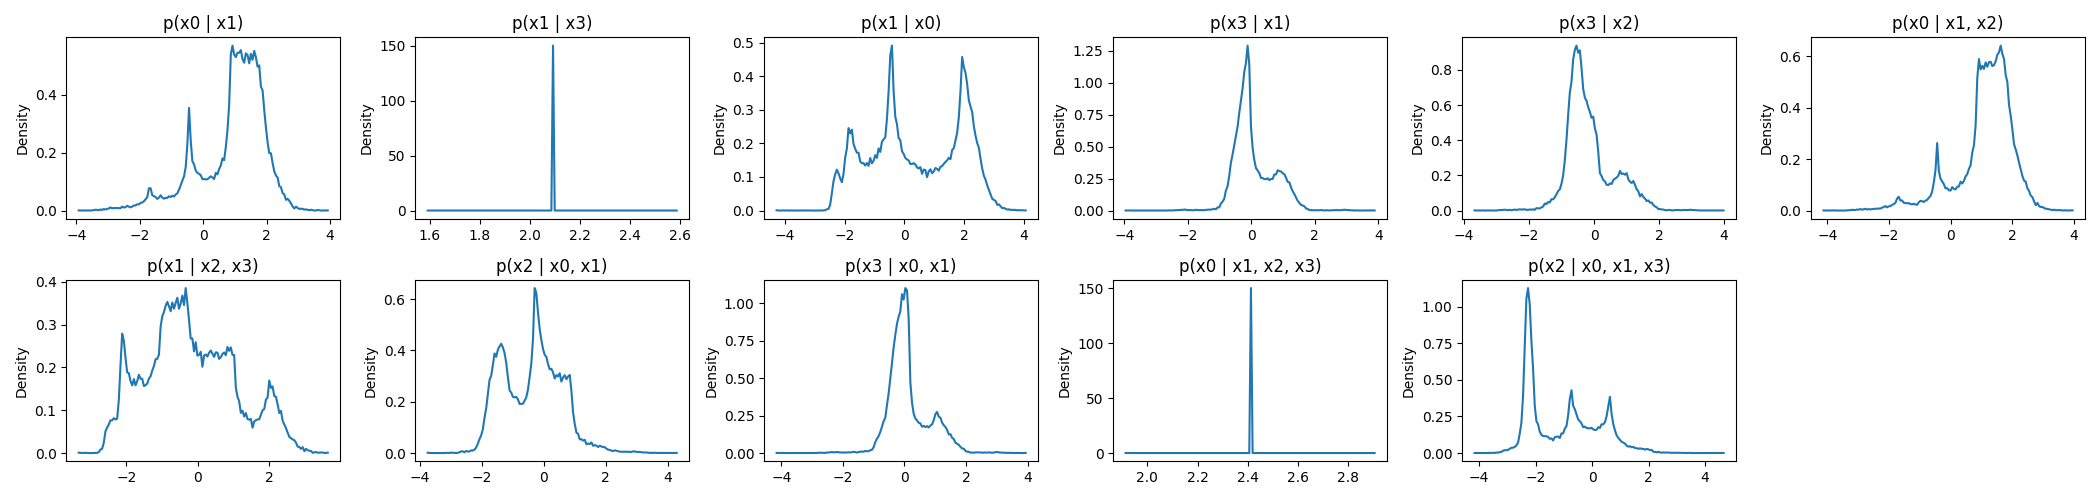
\includegraphics[width=\columnwidth]{images/nonlin-n4-dists.png}
    \caption{An example of a randomly sampled PGM with 4 nodes. Here we plot all the conditional distributions, with one target variable.}
    \label{fig:nonlin-example-pgm-dists}
\end{figure}

\subsubsection{MNIST}

The MNIST benchmark evaluates our framework on real-world image data, providing a practical test of the learned flows on high-dimensional observations. The MNIST dataset consists of 70,000 flattened grayscale handwritten digit images (28$\times$28 pixels, i.e., 784 dimensions) with corresponding labels from 0 to 9.

\paragraph{PGM Structure and Variable Dimensions:}
The MNIST PGM follows a simple causal structure: label $\to$ image, meaning the digit label is the parent of the image data. The variable dimensions are:
\begin{itemize}
    \item \textbf{Image}: 784 dimensions (flattened pixel values, typically normalized to $[0, 1]$)
    \item \textbf{Label}: 10 dimensions (one-hot encoded class labels)
\end{itemize}

\paragraph{Continuous Treatment of Labels:}
While the MNIST labels are inherently categorical (integers from 0 to 9), our flows treat the one-hot encoded label vectors as \textbf{continuous variables}. This easily allows the flow-based models to treat all variables uniformly within the continuous framework.

\paragraph{Dataset Split and Sampling:}
The dataset is partitioned into training (approximately 60,000 samples) and test (approximately 10,000 samples) splits, i.e.\ a 6:1 train/test ratio (the first $6/7$ of the data are used for training). The \texttt{MNISTPGM} class provides conditional sampling via a \texttt{sample()} method:
\begin{itemize}
    \item \textbf{Conditional sampling}: Given a label condition (either as integer index or one-hot encoding), the method samples uniformly from images matching that label within the specified train/test split.
    \item \textbf{Joint sampling}: Without conditions, the method samples both image and label pairs uniformly from the dataset.
\end{itemize}

\subsection{Hyperparameters}
\label{sec:hyperparameters}

Unless otherwise specified, all models (Joint, Static, and Dynamic) were trained using the same budget and optimization settings to ensure a fair comparison.

\begin{table}[h]
\centering
\caption{Hyperparameters used for synthetic PGM benchmarks.}
\begin{tabular}{lr}
\toprule
\textbf{Hyperparameter} & \textbf{Value} \\
\midrule
Optimizer & Adam \\
Initial Learning Rate & $10^{-4}$ \\
Peak Learning Rate & \cam{$10^{-4}$} \\
Ending Learning Rate & \cam{$10^{-6}$} \\
Warmup Steps & 10\% of total \\
Batch Size & \cam{128} \\
Architecture Depth ($D$) & 8 layers \\
\bottomrule
\end{tabular}
\end{table}

\subsection{Baselines}
\label{sec:baselines}

\subsubsection{CAREFL}
We implement Causal Autoregressive Flows (CAREFL) \citep{khemakhem2021causal} as a baseline for structured causal modeling. Unlike the continuous-time ODE flows, CAREFL uses discrete affine transformations. For each node $i$ with parents $pa_i$, the structural equation is:
\begin{equation}
    y_i = g_i(pa_i) \cdot z_i + h_i(pa_i)
\end{equation}
where $z_i \sim \text{Laplace}(0, 1)$ is the noise (following \citealp{khemakhem2021causal} for identifiability), and $g_i, h_i$ are neural networks parameterized to output scaling and shift factors.

\textbf{Implementation:} We use the same \texttt{BlockTriangularStructure} to manage dependencies. The \texttt{log\_prob} is computed by summing the base log-probabilities and the log-determinant terms ($-\sum \log |g_i|$). Sampling is performed by visiting nodes in topological order, computing $g_i, h_i$ from the already sampled parents, and transforming sampled noise $z_i$.

\subsubsection{Guided Baseline}
Our generic baseline is a flow trained on the joint distribution, then conditioned on the required conditions using reconstruction guidance.
The flow is trained on the unconditional joint distribution $p(y)$. During inference, to sample from $p(\Theta | Y_{cond})$, we use reconstruction guidance to steer the ODE trajectories towards the observed values $Y_{cond}$.
\begin{equation}
\mathcal{L}_{rec}(z) = \| z - \hat{z} \|^2 \\
v(z, t) = v_{flow}(z, t) + \gamma \dot\gamma \nabla_{z} \mathcal{L}_{rec}(z)
\end{equation}
where $\gamma$ is from the interpolant noise schedule\cam{, scaled by a guidance strength $\lambda = 7$ (i.e.\ the weight is $-\lambda\gamma\dot\gamma = \lambda(1-t)$ for our interpolant $y_t = t y_1 + (1-t)\epsilon$). This weight is a heuristic: converting a likelihood score into a velocity correction exactly would require the weight $(\alpha^2+\gamma^2)\dot\beta/\beta - (\alpha\dot\alpha + \gamma\dot\gamma) = (1-t)/t$, larger by a factor $1/t$, which diverges at $t=0$ where reconstruction guidance is least accurate. We keep the bounded weight with a tuned strength, as is common for reconstruction guidance}. This method allows for conditional sampling from a model trained only on the joint distribution, but lacks the structural guarantees of our framework.

\section{Appendix: Additional Experiments and Ablations}
\label{app:additional-experiments}

\begin{table}[h]
\centering
\footnotesize
\setlength{\tabcolsep}{4.5pt}
\caption{\textbf{Capability coverage.} No prior method spans both the causal and inference directions for arbitrary DAGs; StructFlow unifies them (and additionally provides an automated compiler and both static/dynamic conditioning, discussed in the text). \cmark~= supported, \xmark~= not supported. ``Explaining-away'' denotes capturing the denser posterior dependencies (moralization) induced at colliders; ``Exact density'' denotes evaluation of model likelihoods by change of variables. $^\dagger$DCM does not provide density evaluation as published; we note that a diffusion model \emph{does} admit exact likelihoods via its probability-flow ODE \citep{song2021scorebased}---which is precisely the continuous-time flow of the last column, and is the sense in which the two rightmost capabilities are not independent (see text).}
\label{tab:capability}
\begin{tabular}{l cccccc}
\toprule
& \rotatebox{90}{Arbitrary DAG~}
& \rotatebox{90}{Causal queries~}
& \rotatebox{90}{Amortized inference~}
& \rotatebox{90}{Explaining-away~}
& \rotatebox{90}{Exact density~}
& \rotatebox{90}{Continuous-time~} \\
\midrule
CAREFL \citep{khemakhem2021causal}              & \cmark & \cmark & \xmark & \xmark & \cmark & \xmark \\
Causal NF \citep{javaloy2023causal}             & \cmark & \cmark & \xmark & \xmark & \cmark & \xmark \\
StrNN \citep{chen2023structured}                & \cmark & \cmark & \xmark & \xmark & \cmark & \xmark \\
DCM \citep{chao2023interventional}              & \cmark & \cmark & \xmark & \xmark & \xmark$^\dagger$ & \xmark \\
Weilbach et al.\ \citep{weilbach2020structured} & \cmark & \xmark & \cmark & \cmark & \cmark & \cmark \\
Zhai et al.\ \citep{jeong_conditional_2025}     & \xmark & \xmark & \cmark & \xmark & \cmark & \cmark \\
\midrule
\textbf{StructFlow (ours)}                       & \cmark & \cmark & \cmark & \cmark & \cmark & \cmark \\
\bottomrule
\end{tabular}
\end{table}


\subsection{MNIST}

We additionally evaluate on MNIST digit generation with the simple two-node structure \texttt{labels}$\to$\texttt{images}, a sanity check at higher dimensionality (784 pixels vs.\ 4 scalar variables in the synthetic PGMs).

\rev{\paragraph{Discrete labels in a continuous flow.} The label block is embedded as a one-hot vector in $\mathbb{R}^{10}$ (standardized by the same mean/variance normalizer as every block; no dequantization noise is added). The flow-matching objective is well-defined for such discrete targets: the linear interpolant $y_t = (1-t)\varepsilon + t\,y_1$ has a density for every $t < 1$ even when $y_1$ is drawn from a mixture of point masses, so the regression target exists almost everywhere and the learned transport concentrates its mass near the one-hot vertices. Sampled labels are decoded by $\arg\max$, and conditioning on a label clamps its (normalized) one-hot block. The colored-MNIST digit variable receives the identical treatment (its color variable, by contrast, is genuinely continuous: a palette color plus Gaussian jitter).}

\paragraph{Results.} All flow-based methods successfully learn the joint and marginal distributions (Figure~\ref{fig:mnist-swd}, Appendix~\ref{app:results}), but dynamic conditioning exhibits notably higher SWD on the conditional $p(\text{images}|\text{labels})$ despite accurately representing the joint. This is a genuine distributional gap rather than an outlier artifact (full diagnostic in Appendix~\ref{app:results}): inspecting samples shows dynamic conditioning produces \emph{perceptually crisp} digits that occasionally render the \emph{wrong class} for the conditioning label---a broadly-distributed conditional error that raises SWD while leaving individual samples realistic. Section~\ref{sec:chain-stiffness} isolates the mechanism behind this gap: dynamic conditioning's clamped condition trajectories leave the training distribution as evidence becomes higher-dimensional and more informative, an error that solver effort does not repair.


\subsection{When Does Structure Help? A Sample-Efficiency Study}
\label{sec:sample-efficiency}

The ablation above shows that the \emph{right} structure (with the co-parent edge) is necessary for correctness. A complementary question is when sparsity is an \emph{advantage}. On the small, well-sampled PGMs of Figure~\ref{fig:inference-nonlinear-pgm}, an unstructured flow can match a structured one because it has enough data to fit its extra (spurious) dependencies harmlessly. Structure should matter most when data are scarce, where its hard sparsity acts as an inductive bias that reduces variance.

We test this on a linear-Gaussian chain $x_0 \to x_1 \to \cdots \to x_5$, inferring $p(x_0,\dots,x_4 \mid x_5)$ (the exact posterior is Gaussian). We compare two static flows of the same family that differ only in connectivity: the \textbf{sparse} structure produced by our compiler ($5$ edges) and a \textbf{dense}, fully-connected flow ($15$ edges). Both are trained identically across a range of training-set sizes $N$, and we measure the $2$-Wasserstein distance between each flow's posterior and the exact posterior---an interpretable, zero-based metric.

Figure~\ref{fig:sample-efficiency} shows the result. The structured (sparse) flow is more accurate at every $N$, and the gap is largest in the low-data regime ($1.9\times$ lower error at $N{=}64$), narrowing as $N$ grows and the dense flow accumulates enough data to suppress its spurious dependencies. This is the expected behaviour of a correct inductive bias, and it explains the comparable performance of structured and unstructured flows in the well-sampled setting of Figure~\ref{fig:inference-nonlinear-pgm}: structure is most valuable precisely when data are limited. We present this single linear-Gaussian chain---which isolates the mechanism against an exact Gaussian posterior---as an illustration of the bias--variance trade-off that hard sparsity induces, not as a quantitative law; the magnitude of the advantage will depend on graph density and dimensionality.

\begin{figure}[t]
    \centering
    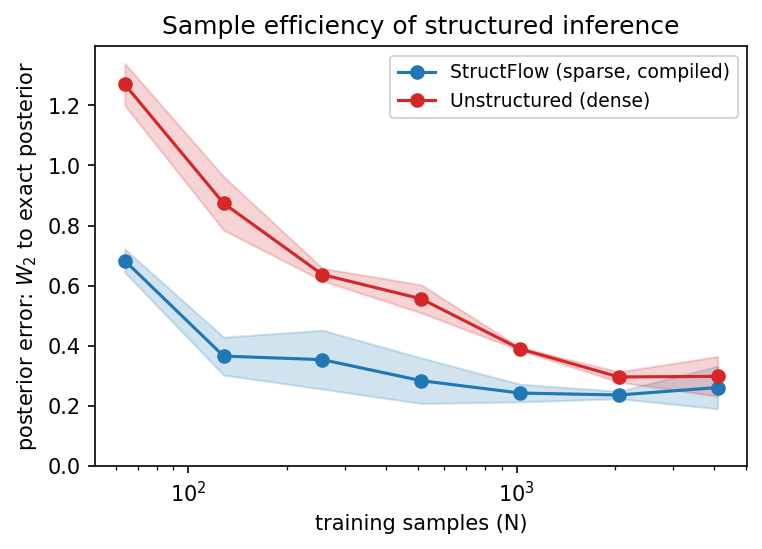
\includegraphics[width=0.55\columnwidth]{images/ablations/sample_efficiency.png}
    \caption{\textbf{Structure as an inductive bias.} Posterior error ($2$-Wasserstein to the exact posterior) versus training-set size for a linear-Gaussian chain: the compiler's sparse structure (blue) outperforms an unstructured dense flow (red) of the same family, with the largest advantage when data are scarce; the two converge as $N$ grows (bands: $\pm 1$ s.d.\ over seeds).}
    \label{fig:sample-efficiency}
\end{figure}

\subsection{Ablation: Does the Backbone Matter?}
\label{sec:backbone-ablation}

The comparisons above vary the \emph{structure} while holding the backbone fixed. Because
diffusion models and flow matching are the same object class up to reparameterization
(Section~\ref{par:backbone}), the complementary experiment is to vary the backbone while
holding the structure fixed. We therefore replace each block's continuous-time velocity field
with a per-node denoising diffusion model conditioned on the block's parents---the
construction of DCM \citep{chao2023interventional} and Diff-SCM
\citep{sanchez2022diffusion}---and re-run causal alignment on the same graphs, the same data,
and a matched parameter budget. Abduction uses DDIM inversion, as in those works. We present
this as an \emph{ablation of our own framework}, not as a competitor comparison: the question
is whether the compiler or the backbone is load-bearing.

Proposition~\ref{prop:abduction-error} makes a falsifiable prediction. Interventional queries
require no inversion, so the two backbones should agree; counterfactual queries require
abduction, where the CNF's error is solver tolerance at fixed weights while DDIM inversion
carries a first-order term in the step size. We therefore report accuracy as a function of
sampling compute (number of function evaluations, NFE) rather than at a single operating
point, since a single-NFE comparison cannot distinguish a backbone difference from a budget
choice.

Figure~\ref{fig:backbone-nfe} shows the result on the nonlinear $4$-node benchmark (5 PGM seeds, matched parameter budgets, NFE counted as \emph{network evaluations} per sample---RK4 costs four per step, DDIM one---so the axis is compute, not step count). Three observations. \emph{Interventional queries}: the backbones agree at moderate-to-high NFE (${\geq}16$; SWD $0.023$--$0.025$), with the diffusion variant degrading below that because its forward sampler is itself first-order, while the CNF remains flat even at a single RK4 step. \emph{Abduction error}---the direct measurement of Proposition~\ref{prop:abduction-error}---separates the backbones cleanly: the diffusion variant's reconstruction error $\lVert \mathrm{invert}(\mathrm{forward}(u)) - u \rVert$ decays at almost exactly first order in NFE (halving per doubling), exactly as predicted for published DDIM inversion, while the CNF's decays at roughly second order and ends ${\sim}55\times$ lower at NFE $128$. \emph{Counterfactual SWD} rises $10\times$ for the diffusion backbone as NFE falls from $128$ to $4$, versus $2.4\times$ for the CNF; one honest nuance is that at NFE ${\geq}64$ the diffusion variant's counterfactual SWD is slightly \emph{below} the CNF's ($0.0047$ vs $0.0085$) despite its far larger pointwise abduction error---SWD is a distributional metric and does not penalize an inversion bias that approximately preserves the noise distribution, which is why the abduction panel, not the counterfactual panel, is the proposition's direct test. Finally, the inference-mode columns are empty for the diffusion backbone by construction: per-node diffusion supplies no amortized posterior, no moralization, and no conditional density (its NLL/KL entries correctly surface as unavailable). Training differs in one respect we could not match: the flow variants use minibatch OT coupling, which has no diffusion analogue.

\begin{figure*}[t]
    \centering
    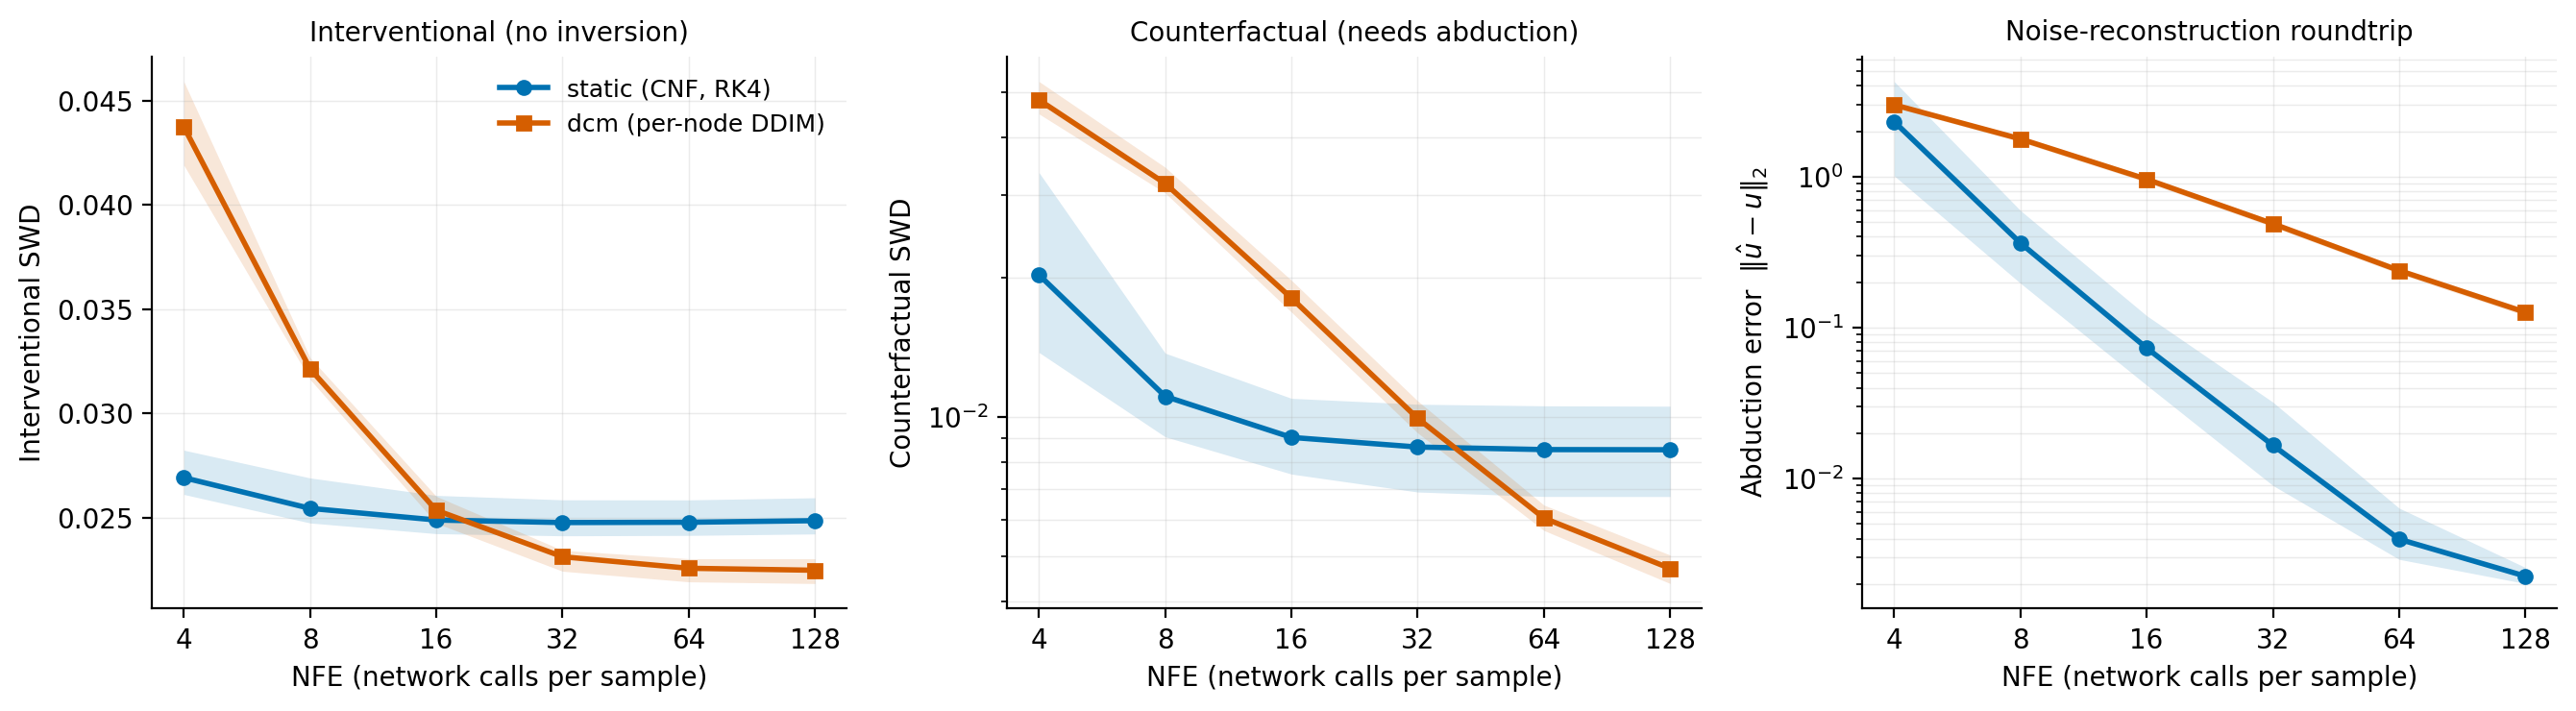
\includegraphics[width=\textwidth]{images/ablations/backbone_nfe.png}
    \caption{\textbf{Backbone ablation on nonlinear 4-node PGMs} (mean $\pm$ range over 5 PGM seeds; $x$-axis is measured network evaluations per sample). \textbf{Left:} interventional SWD---backbones agree for NFE $\geq 16$. \textbf{Middle:} counterfactual SWD---the diffusion backbone degrades far more steeply at low NFE. \textbf{Right:} abduction reconstruction error---first-order decay for DDIM inversion versus ${\sim}$second-order for the CNF, the direct measurement of Proposition~\ref{prop:abduction-error}.}
    \label{fig:backbone-nfe}
\end{figure*}

The outcome we expect makes the paper's argument better than a win would. If the two
backbones tie on interventional queries and the diffusion variant has no inference-mode
entries at all, that is direct evidence that the compiled structure---not the choice of
continuous-time generative model---is what delivers the capabilities of
Table~\ref{tab:capability}.


\subsection{Inference Alignment: Amortized Probabilistic Inference}

For Inference Alignment, we use StructFlow to ``invert'' the DAG---edges point from children to parents, with additional edges via moralization. This enables efficient sampling from posterior distributions $p(\text{parents} | \text{children})$.

\paragraph{Results.} Figure \ref{fig:inference-nonlinear-pgm} shows that our structured flows can effectively learn to perform probabilistic inference, providing accurate amortized inference over the model's latent variables. On these small, well-sampled nonlinear PGMs all methods perform comparably---including the unstructured \textit{Guided} baseline. This is expected rather than contradictory: the Guided flow places dependencies between \emph{all} variables, so it implicitly contains the moral edges that the posterior requires. The ablation in Section~\ref{sec:moralization-ablation} isolates this effect, showing that the relevant structural ingredient is exactly the moralization our compiler performs; and Section~\ref{sec:sample-efficiency} shows that the benefit of \emph{sparse} structure (over a dense, unstructured flow) emerges when training data are limited. The same qualitative picture holds on larger random $8$-node nonlinear PGMs, confirming the framework is not limited to very small graphs (Appendix~\ref{app:results}, Figure~\ref{fig:inference-n8}); the binding constraint on scaling further is \emph{evaluation}---generating MCMC ground truth for every conditional query (Section~\ref{sec:future_work})---not training.

\subsection{Ablation: Is Moralization Necessary?}
\label{sec:moralization-ablation}

\rev{The compiled inference structure contains a dependency between the parents of a collider (the ``moral'' edge, produced by the d-separation step under the compiled ordering) to capture the posterior dependencies induced by ``explaining away''.} We test whether this edge is truly necessary on a linear-Gaussian collider $A \to C \leftarrow B$ with $A, B \sim \mathcal{N}(0,1)$ and $C = A + B + \sigma \epsilon$. Observing $C$ induces a strong negative correlation between $A$ and $B$, and the exact posterior $p(A, B \mid C)$ is available in closed form.

We compile the inference flow for the query $p(A, B \mid C)$ and compare the StructFlow architecture (which adds the moral edge $A\!-\!B$) against an ablated architecture with that edge removed---so the flow is forced to factorize as $p(A \mid C)\,p(B \mid C)$. Both are trained identically on the same joint samples.

Figure~\ref{fig:moralization-ablation} shows the outcome. The ablated (non-moralized) flow recovers the correct posterior \emph{marginals} but is structurally incapable of representing the posterior correlation, yielding $\mathrm{corr}(A, B \mid C) \approx 0$. The moralized StructFlow recovers it closely ($-0.94$ vs.\ the analytic $-0.92$; the small overshoot is within the seed-to-seed variation of the learned flow). \rev{This isolates the contribution of the compiled co-parent dependency: it is not a heuristic convenience but a requirement for faithfully representing collider posteriors.} We demonstrate the effect on this canonical collider because it admits a closed-form posterior, but the conclusion is \emph{structural} rather than specific to this instance: without an edge between two colliding parents, a block-triangular flow has no computational path to couple them, so it cannot represent any induced posterior correlation regardless of the underlying mechanism.

\begin{figure}[t]
    \centering
    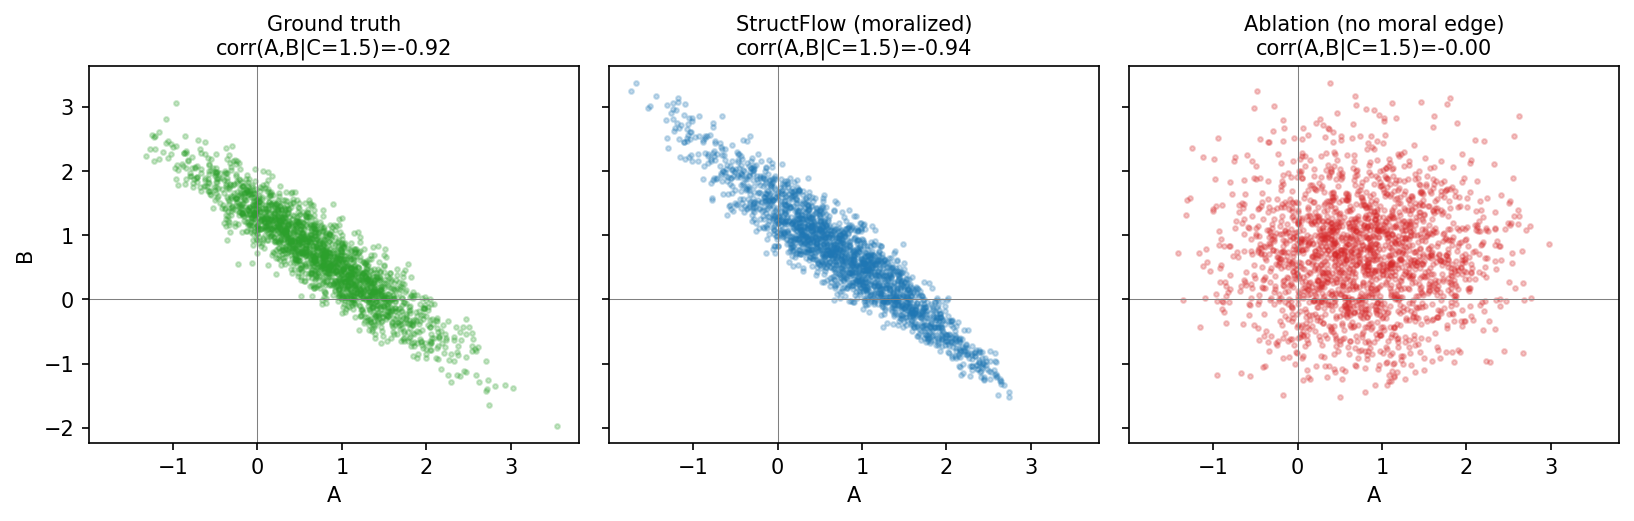
\includegraphics[width=0.82\columnwidth]{images/ablations/moralization_collider.png}
    \caption{\textbf{The compiled co-parent dependency is necessary for explaining-away.} Posterior samples of $p(A, B \mid C{=}1.5)$ for the collider $A \to C \leftarrow B$. \textbf{Left:} analytic ground truth (strong negative correlation). \textbf{Middle:} StructFlow with the moral edge recovers the correlation. \textbf{Right:} the ablation without the moral edge captures the marginals but collapses the correlation to $\approx 0$.}
    \label{fig:moralization-ablation}
\end{figure}

\subsection{Ablation: Separating Moralization from d-Separation}
\label{app:ordering-ablation}
\rev{
The compiler's two graph-processing steps play different roles, and this ablation separates them. The dependency set of a compiled structure is constructed \emph{entirely} by the d-separation step: for any ordering with the conditions as a prefix, each block's parents are exactly the predecessors it is not d-separated from in the original DAG. Moralization enters only through the breadth-first traversal that \emph{chooses} the ordering---marrying co-parents so that explaining-away partners are visited adjacently. We therefore compile the leaf-conditioned posterior of each test graph under three ordering policies, holding the d-separation step fixed: (a)~the moral-BFS ordering (the compiler as shipped), (b)~a no-moralization ordering (conditions first, remaining variables in reverse topological order), and (c)~$20$ random orderings with the conditions kept as a prefix.

Two findings. \emph{First, correctness never depends on the ordering policy}: on the collider of Section~\ref{sec:moralization-ablation}, the co-parent dependency appears in the compiled structure under \emph{every} ordering tested---it is forced by d-separation ($A \not\perp_d B \mid C$), so the posterior dependencies that Figure~\ref{fig:moralization-ablation} shows to be necessary are supplied by the d-separation step regardless of how the ordering was chosen. \emph{Second, the ordering policy controls sparsity}: across colliders, chains ($n \in \{4, 8\}$), and $15$ random DAGs ($n \in \{4, 6, 8\}$, five seeds each), the moral-BFS ordering never yields more compiled dependencies than the alternatives and yields strictly fewer on $11$ of $18$ graphs (mean $12.8$ edges vs.\ $13.9$ for the no-moralization ordering and $14.3$ for the random-order median; on the $8$-chain, adversarial orderings inflate $7$ edges to $13$). Since sparsity is the inductive bias behind the sample-efficiency results of Section~\ref{sec:sample-efficiency}, moralization earns its place as the ordering heuristic---but the compiled dependencies, and hence correctness, come from d-separation alone. The ablation is reproduced by \texttt{scripts/ablations/ordering\_ablation.py}.}

\subsection{Validating the NUTS References}
\label{app:nuts-validation}
\rev{
The nonlinear inference benchmarks are scored against NUTS reference posteriors, so their accuracy is load-bearing. The reference protocol draws each sample from an \emph{independent} chain (window adaptation for $250$ steps, then a single kept state, vectorized over chains), so the ensemble carries no autocorrelation but relies entirely on warmup convergence from a prior initialization---a failure of which would bias every chain identically and be invisible to within-chain diagnostics. We therefore validate the protocol three ways, on the benchmark graph family at both node dimensions used in the paper and at $n{=}16$ beyond it (\texttt{scripts/ablations/nuts\_validation.py}). \emph{Closed-form anchor}: on linear-Gaussian instances, where the exact posterior is available, the reference ensemble's Bures-$W_2$ to the analytic posterior is $2$--$4\%$ of the posterior scale at every benchmark size (up to $n{=}8$, $d{=}8$: $64$-dimensional joints), consistent with the finite-ensemble Monte-Carlo floor. \emph{Warmup sensitivity}: increasing warmup $4\times$ (and, at $n \le 8$, $16\times$) moves the ensemble by \emph{less} than its own resampling noise (SWD $0.030$--$0.074$ between warmup settings vs.\ half-split floors of $0.060$--$0.113$)---$250$ steps is converged. \emph{Simulation-based calibration} \citep{talts2018validating}: over $300$ replications per graph, ranking the joint draw among $99$ reference draws, the per-dimension $\chi^2$ uniformity $p$-values are consistent with uniform ranks on every benchmark-family graph (minimum $0.03$ across $40$ tested dimensions, as expected under uniformity). We conclude the reference error sits at the Monte-Carlo floor of the ensemble sizes used, well below the method differences the benchmarks measure.

The validation also has teeth: pushed beyond the benchmarks, to a \emph{linear} $n{=}16$, $d{=}8$ graph ($128$-dimensional joint), the protocol fails outright---anchor $W_2 \approx 52\times$ the posterior scale, SBC $p$-values below $10^{-13}$---because $16$ layers of random linear maps produce an ill-conditioned joint whose scale disparities defeat warmup adaptation from a prior initialization (diagnostically, ensembles at different warmup budgets agree with each other far better than either agrees with its own half-splits: the chains are frozen where they start). The nonlinear $n{=}16$ counterpart, whose spline mechanisms keep the joint well-conditioned, passes all checks. Accordingly, any linear-Gaussian evaluation at $n{=}16$ must use the closed-form conditionals rather than the MCMC reference path.}

\subsection{Amortized Inference vs.\ MCMC}
\label{sec:amortization}

A practical advantage of Inference Alignment is \emph{amortization}: the flow is trained once, after which any posterior query $p(\text{targets} \mid \text{conditions}{=}c)$ is answered with a single fast ODE solve, whereas a classical sampler such as the No-U-Turn Sampler (NUTS) must run a fresh Markov chain for every observed value $c$. On a nonlinear collider, Figure~\ref{fig:amortization} (right) confirms that StructFlow's amortized posterior and a NUTS reference agree closely (mean Sliced Wasserstein distance $0.0014$ across queries), while Figure~\ref{fig:amortization} (left) shows the wall-clock trade-off: StructFlow pays a one-time training cost but is roughly $11\times$ faster \emph{per query}, so its cumulative cost overtakes per-query MCMC after a crossover of $K^\star \approx 22$ queries. The specific speedup and crossover are setup-dependent (Appendix~\ref{app:experiments}), but the qualitative conclusion is general: structured amortized inference is preferable whenever many posterior queries must be answered for the same model.

\begin{figure}[t]
    \centering
    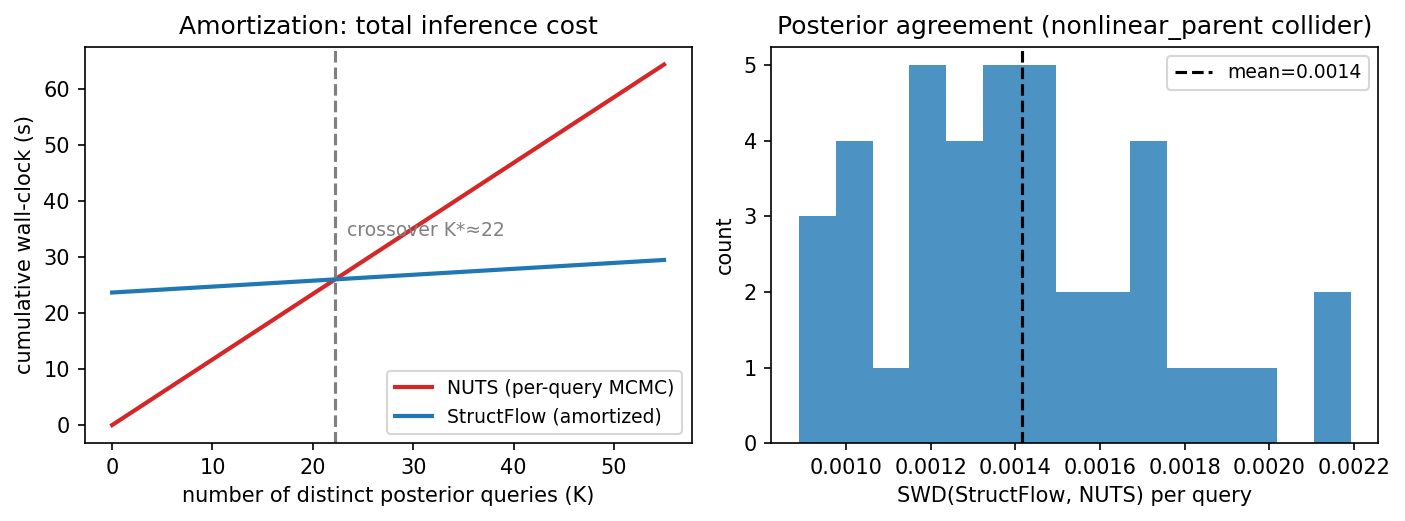
\includegraphics[width=0.95\columnwidth]{images/ablations/amortization_vs_nuts.png}
    \caption{\textbf{Amortized inference vs.\ per-query MCMC} on a nonlinear collider. Left: cumulative wall-clock versus the number of distinct posterior queries; the amortized flow overtakes NUTS after $K^\star \approx 22$ queries. Right: per-query agreement between StructFlow and the NUTS reference (Sliced Wasserstein distance).}
    \label{fig:amortization}
\end{figure}


\subsection{Colored-MNIST: Intervene-vs-Observe Heatmaps}

\begin{figure*}[t]
    \centering
    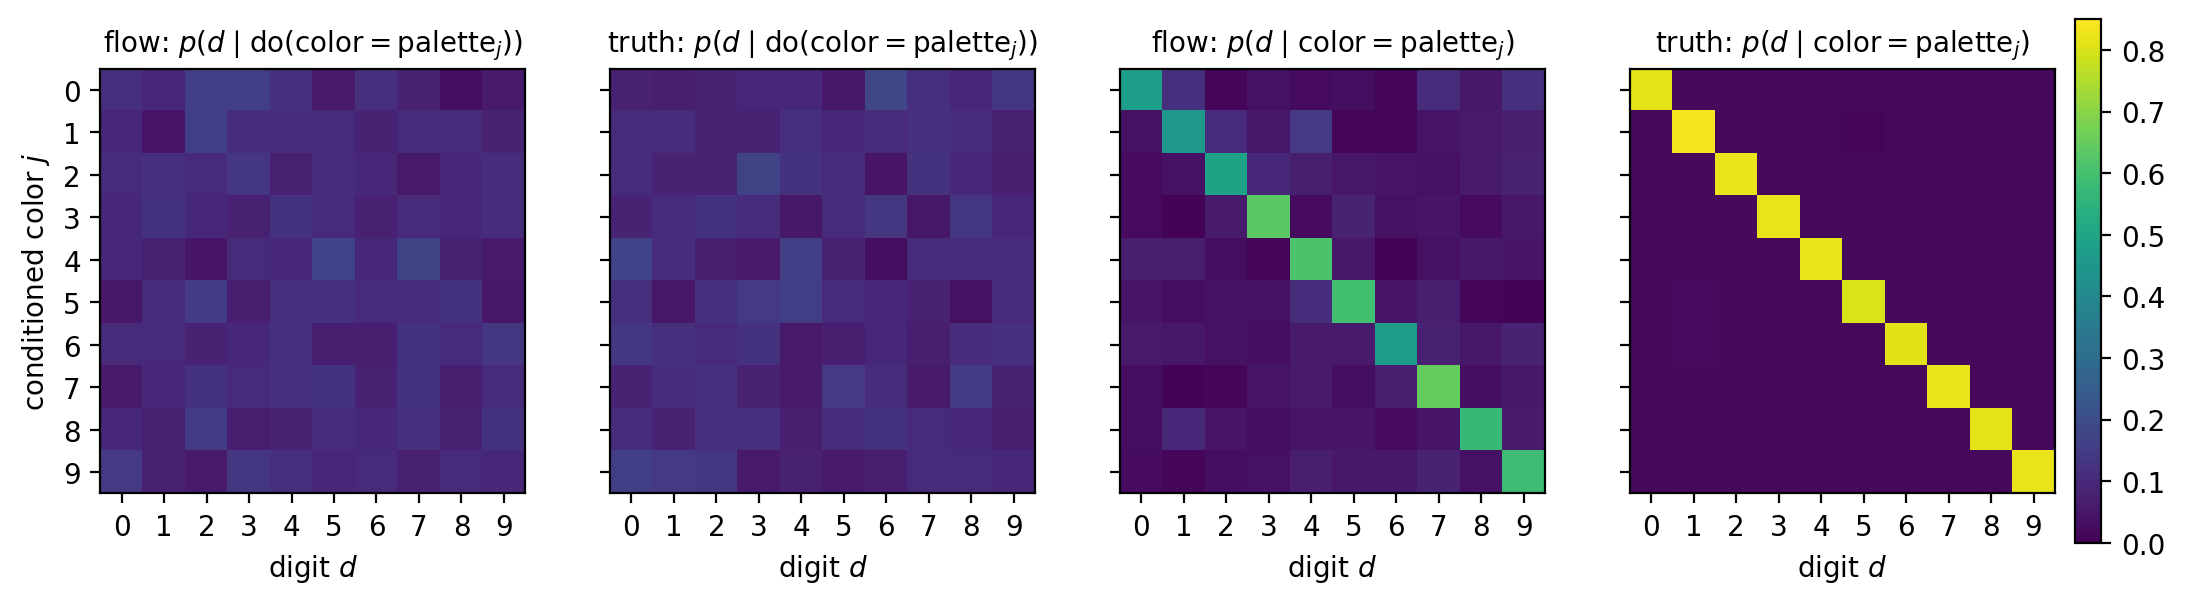
\includegraphics[width=\textwidth]{images/colored_mnist_conv_heatmaps.png}
    \caption{\textbf{Intervening vs.\ conditioning on Colored-MNIST.} Digit marginals for each conditioned palette color $j$ (rows). Under $\mathrm{do}(\mathrm{color})$ (left pair) the digit distribution is unchanged---both the flow and the sampled ground truth are uniform. Under observational conditioning (right pair) the posterior concentrates on the color-correlated digit: the flow (third panel) recovers the diagonal of the exact analytic posterior (fourth panel; noise-free because it is computed in closed form, whereas the truth-interventional panel is sampled).}
    \label{fig:colored-mnist-heatmaps}
\end{figure*}

\subsection{Colored-MNIST at $\rho = 1$: Zero-Shot Counterfactuals}
\label{app:colored-mnist-rho1}

\begin{figure}[t]
    \centering
    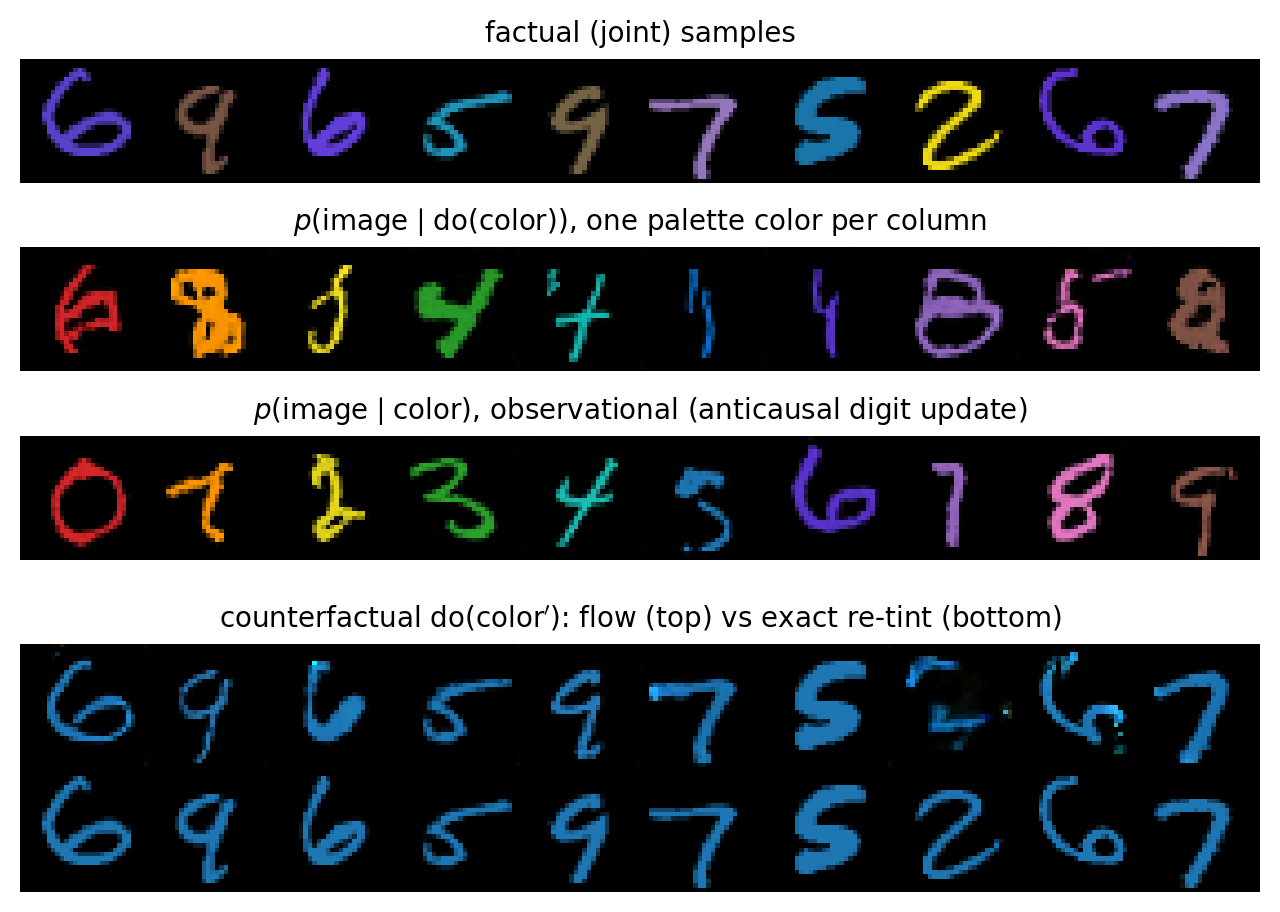
\includegraphics[width=0.6\columnwidth]{images/colored_mnist_rho1_strips.png}
    \caption{\textbf{Colored-MNIST with deterministic colors ($\rho = 1$).} Same layout as Figure~\ref{fig:colored-mnist-strips}, retrained on data where every digit always wears its palette color, so no off-diagonal (digit, color) pair ever appears in training. Row 2: interventional samples still extrapolate to every unseen combination. Row 3: the observational posterior is now a point mass, and the flow produces exactly one digit per color. Row 4: counterfactual re-coloring is now genuinely zero-shot mechanism transfer; most samples match the exact re-tint, and the failures (e.g.\ the thick `2') are abduction failures---inverting a factual image through a flow whose training support never dissociated digit from color.}
    \label{fig:colored-mnist-rho1}
\end{figure}

\newpage
\section{Appendix: Extended Results}
\label{app:results}

\subsection{Linear versus non-linear}

We expect CAREFL to do well on the linear PGM problem as the structure of the PGM matches CAREFL's inductive bias: affine transformations of a fixed base distribution. But since these assumptions are restrictive, we expect CAREFL to perform poorly on the non-linear PGM problem. \cam{The results (Figures~\ref{fig:swd-linear-v-nonlinear} and~\ref{fig:counterfactual-linear-v-nonlinear}) bear this out: on the linear benchmarks CAREFL is the strongest method on counterfactual queries---abduction through its exactly-matched affine inverse is nearly exact---although Static and the universal flow lead on interventional queries; on the nonlinear benchmarks CAREFL falls behind the structured CNFs on both. Dynamic conditioning is close to Static on the nonlinear graphs (interventional SWD within $15\%$) but clearly worse on the linear ones (${\sim}2.6\times$ on interventional queries), where the strong linear dependence between blocks makes the residual bias of the minibatch per-block coupling largest (Section~\ref{sec:chain-stiffness}).}

\begin{figure*}[hbt!]
    \centering
    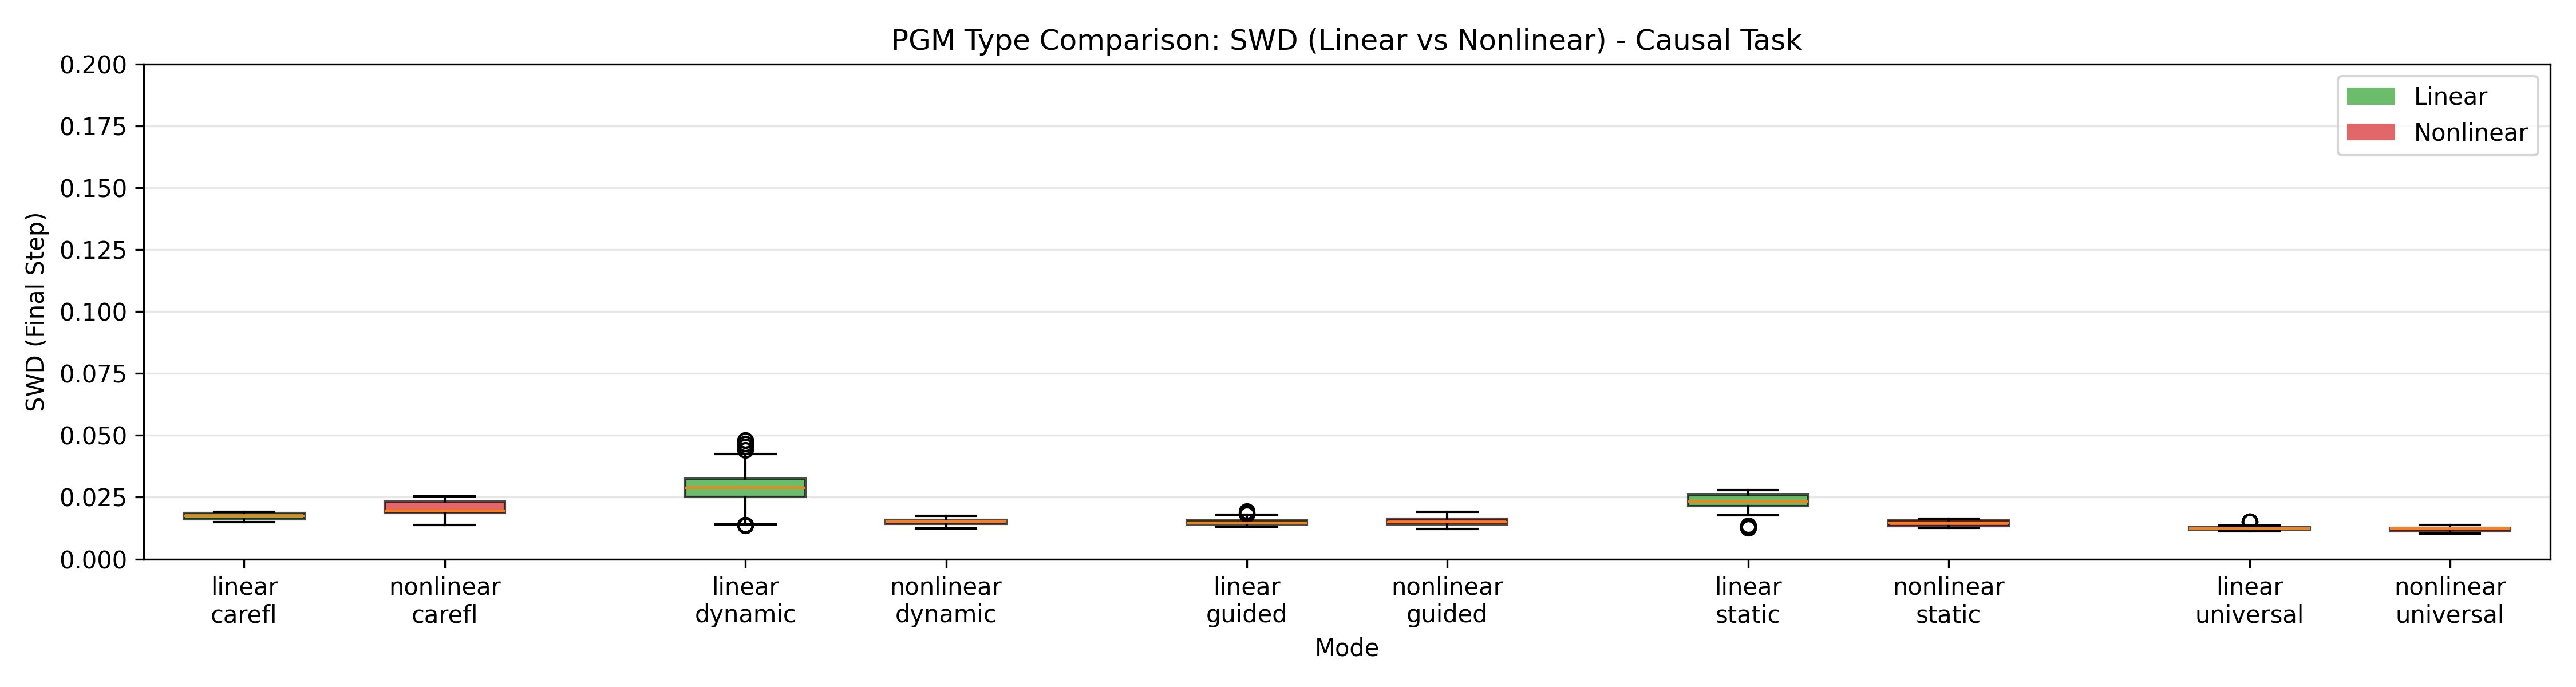
\includegraphics[width=\textwidth]{images/experimental_figures/pgm_type_comparison_swd_task_causal_conditional.png}
    \caption{\textbf{Interventional Query Results.} Sliced Wasserstein Distance for interventional distributions $p(y \mid \mathrm{do}(x))$ on linear and nonlinear PGMs (these coincide with the observational conditionals $p(y \mid x)$ for the evaluated query family; see Section~\ref{sec:experiments}). Results aggregated over 5 PGM seeds and 5 learner seeds.}
    \label{fig:swd-linear-v-nonlinear}
\end{figure*}

\begin{figure*}[hbt!]
    \centering
    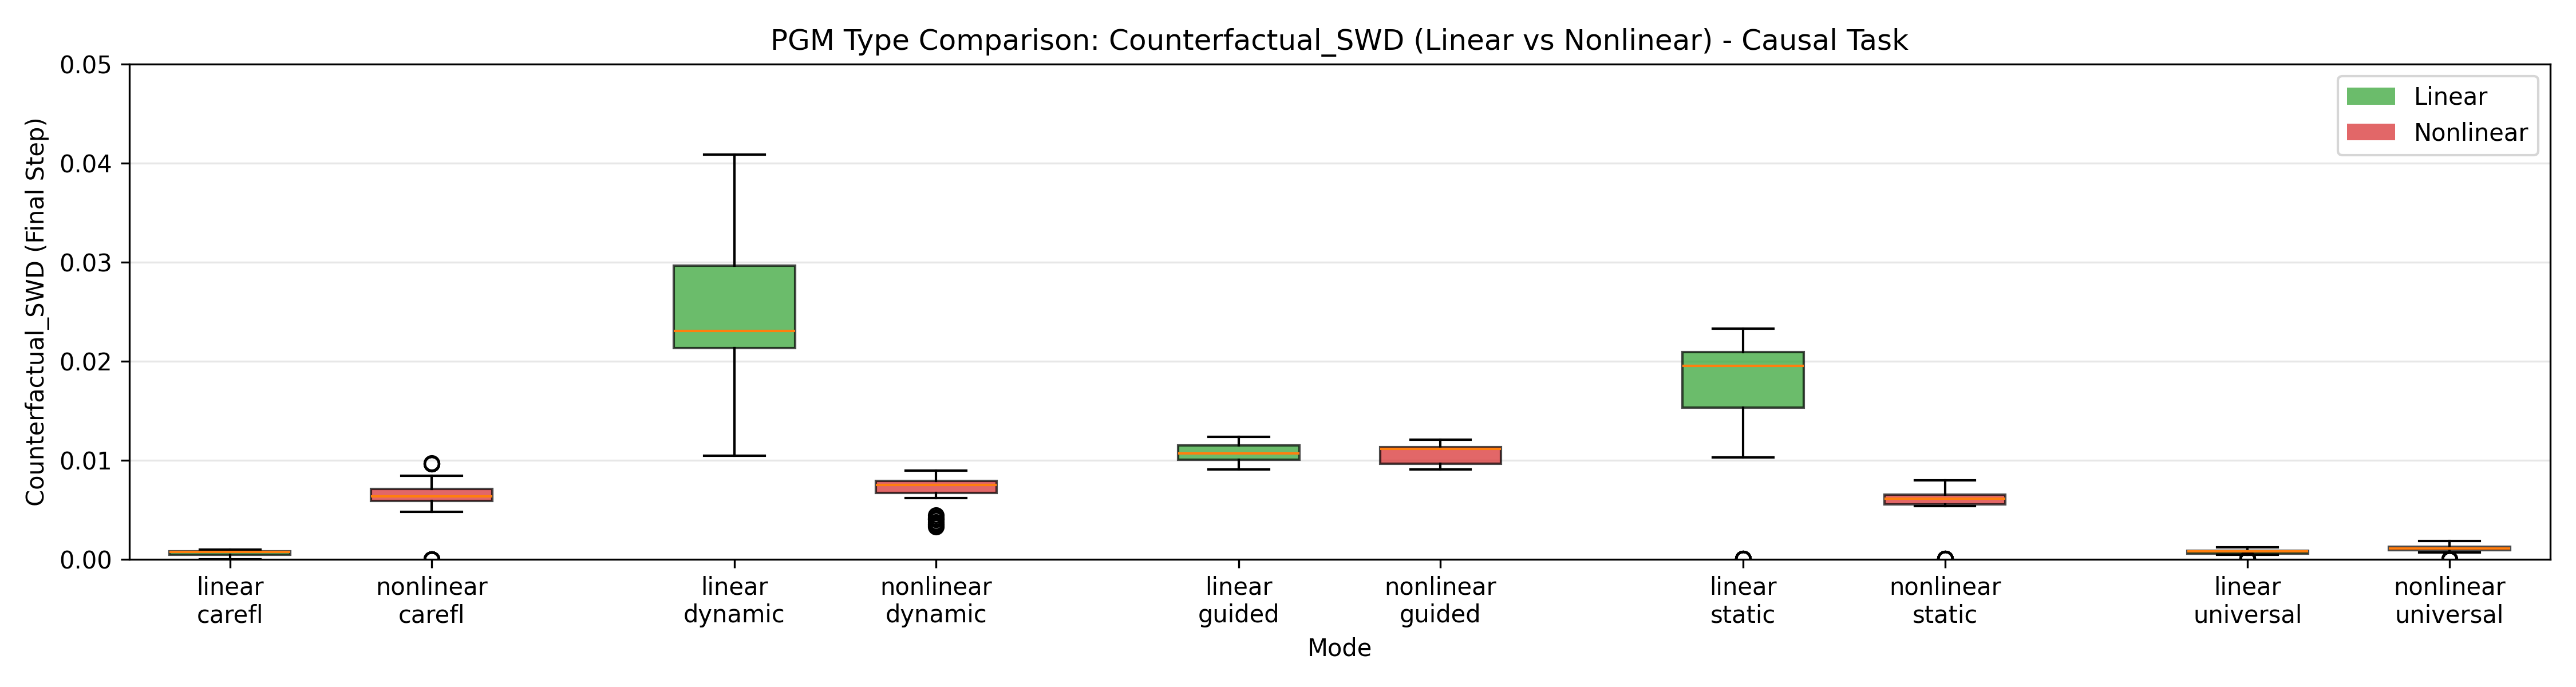
\includegraphics[width=\textwidth]{images/experimental_figures/pgm_type_comparison_counterfactual_swd_task_causal_conditional.png}
    \caption{\textbf{Counterfactual Query Results.} Sliced Wasserstein Distance for counterfactual distributions on linear and nonlinear PGMs. Aggregated over 5 PGM seeds and 5 learner seeds.}
    \label{fig:counterfactual-linear-v-nonlinear}
\end{figure*}

\subsection{KL divergence on linear-Gaussian causal queries}
\label{app:kl-linear}

On the linear-Gaussian benchmarks the ground-truth conditionals are available in closed form, so the causal queries can additionally be scored by KL divergence, which puts the (deliberately small) normalized SWD values of Section~\ref{sec:experiments} on a calibrated scale. Table~\ref{tab:linear4-kl} reports median scores on the $4$-node linear benchmark, aggregated over conditional causal queries, $5$ PGM seeds and $5$ learner seeds. \cam{Among the methods that define a tractable conditional density, KL and SWD agree on interventional queries that Static and the universal flow are best (near-tied by SWD; KL favors the universal flow) and Dynamic is worst; guided sampling defines no conditional density for most queries, so its KL is omitted. On counterfactuals SWD ranks CAREFL first, then the universal flow and Static, with Dynamic far behind. The log-ratio column (see below) instead puts Static and the universal flow nearest zero and CAREFL and Dynamic at ${\sim}0.2$; it measures agreement of the interventional densities, not counterfactual accuracy, so the two need not agree.}

A remark on what the counterfactual columns measure. Our factuals are \emph{fully observed}, so by Remark~\ref{rem:density-scope} each counterfactual is a point mass and has no density of its own. The ``Cf.'' entries are therefore \emph{not} divergences between counterfactual distributions: each model evaluates the density of its own \emph{mutilated (interventional)} distribution at the counterfactual point, and the reported score is the mean log-ratio of the true and learned interventional densities over the factual population---a calibration diagnostic asking whether the two mutilated models agree along the manifold where counterfactuals land. Read this way, the column is consistent with Remark~\ref{rem:density-scope}; \cam{it is a calibration check, and it does not rank methods by counterfactual accuracy.}

\begin{table}[h]
\centering
\caption{\textbf{KL divergence versus SWD on the $4$-node linear-Gaussian benchmark} (causal task, conditional queries; median over queries, $5$ PGM seeds and $5$ learner seeds). ``Int.''\ denotes interventional queries; ``Cf.''\ entries are interventional-density log-ratios evaluated at the counterfactual points (see text---the counterfactual itself is a point mass under full observation, Remark~\ref{rem:density-scope}). \cam{Being a mean log-ratio rather than a divergence, a Cf.\ entry can be slightly negative.} KL corroborates the SWD ordering of the density-bearing methods; guided sampling has no tractable conditional density, so KL is unavailable for it.}
\label{tab:linear4-kl}
\begin{tabular}{lrrrr}
\toprule
\textbf{Method} & \textbf{Int.\ SWD} & \textbf{Int.\ KL} & \textbf{Cf.\ SWD} & \textbf{Cf.\ KL} \\
\midrule
Static    & 0.0027 & 0.055 & 0.0009 & $-0.024$ \\
Universal & 0.0028 & 0.025 & 0.0004 & 0.023 \\
Guided    & 0.0042 & ---   & ---    & ---   \\
CAREFL    & 0.0052 & 0.221 & 0.0003 & 0.214 \\
Dynamic   & 0.0071 & 0.232 & 0.0065 & 0.200 \\
\bottomrule
\end{tabular}
\end{table}

\subsection{Learning the joint distribution: causal structure versus inference structure}

Is one direction (causal versus inference) better at learning the joint distribution than the other? No: for every flow-based method the two structures give joint SWDs within $3\%$ of each other (e.g.\ Static $1.30$ vs.\ $1.32 \times 10^{-3}$), and CAREFL is $5\%$ lower with the inference structure, while remaining about twice the others' error in both (Figure~\ref{fig:nonlinear-joint}).

\begin{figure}[hbt!]
    \centering
    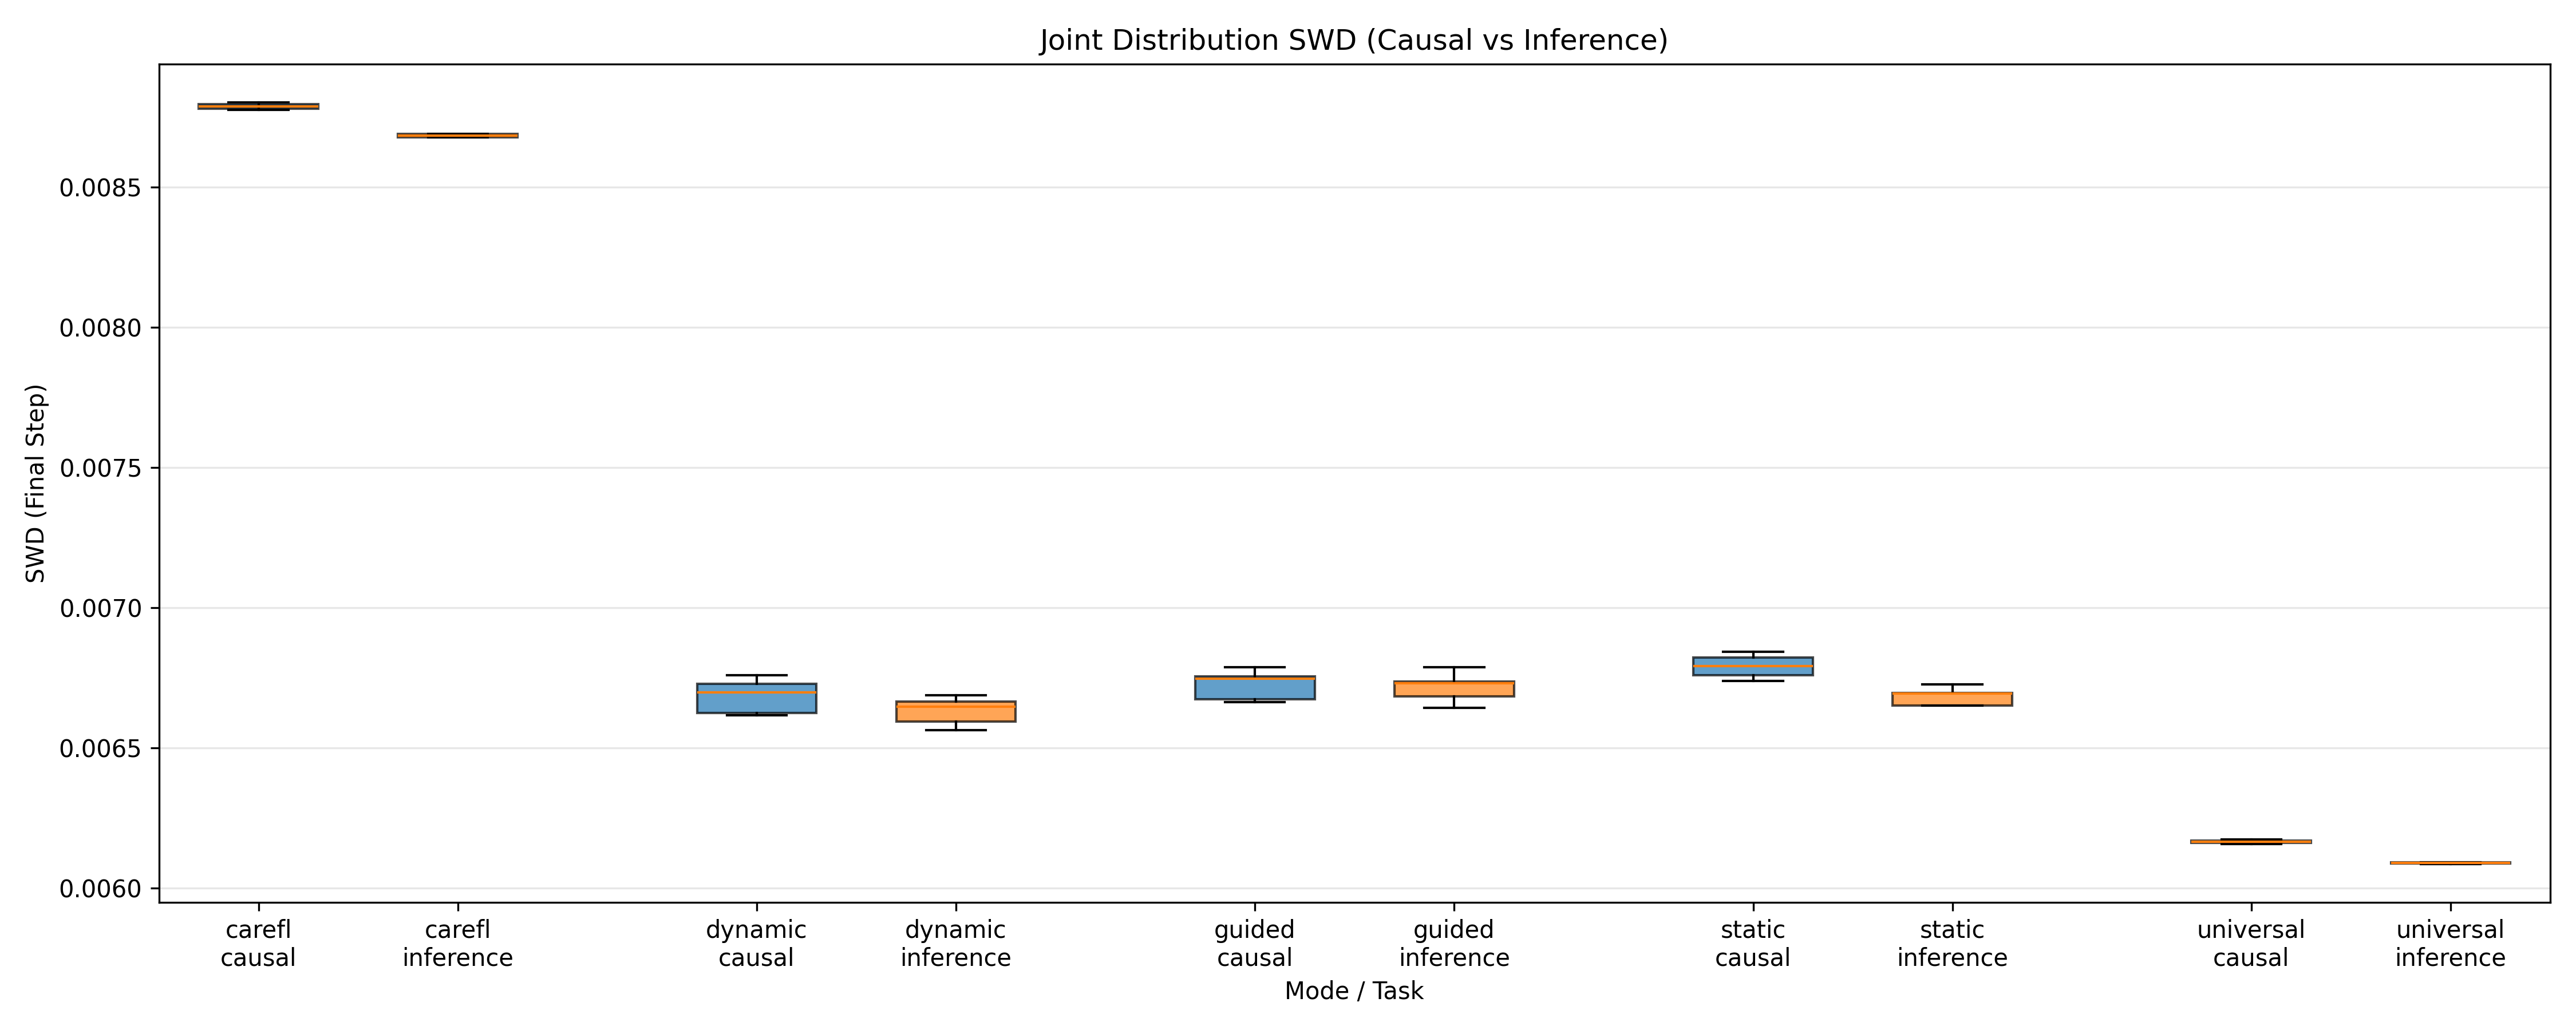
\includegraphics[width=0.8\textwidth]{images/experimental_figures/nonlinear/task_comparison_swd_joint.png}
    \caption{\textbf{Joint-distribution SWD by compiled structure} on the nonlinear $4$-node PGMs. For each method, the left box is the model trained with the causal structure and the right box the model trained with the inference structure; each box shows the spread over $5$ learner seeds, each averaged over $5$ PGM seeds.}
    \label{fig:nonlinear-joint}
\end{figure}

\subsection{Granular PGM metrics}

Figures~\ref{fig:causal-nonlinear-pgm-queries} and~\ref{fig:inference-nonlinear-pgm-queries} break the aggregated nonlinear results of Figure~\ref{fig:pgm-results} down by query.

\begin{figure}[hbt!]
    \centering
    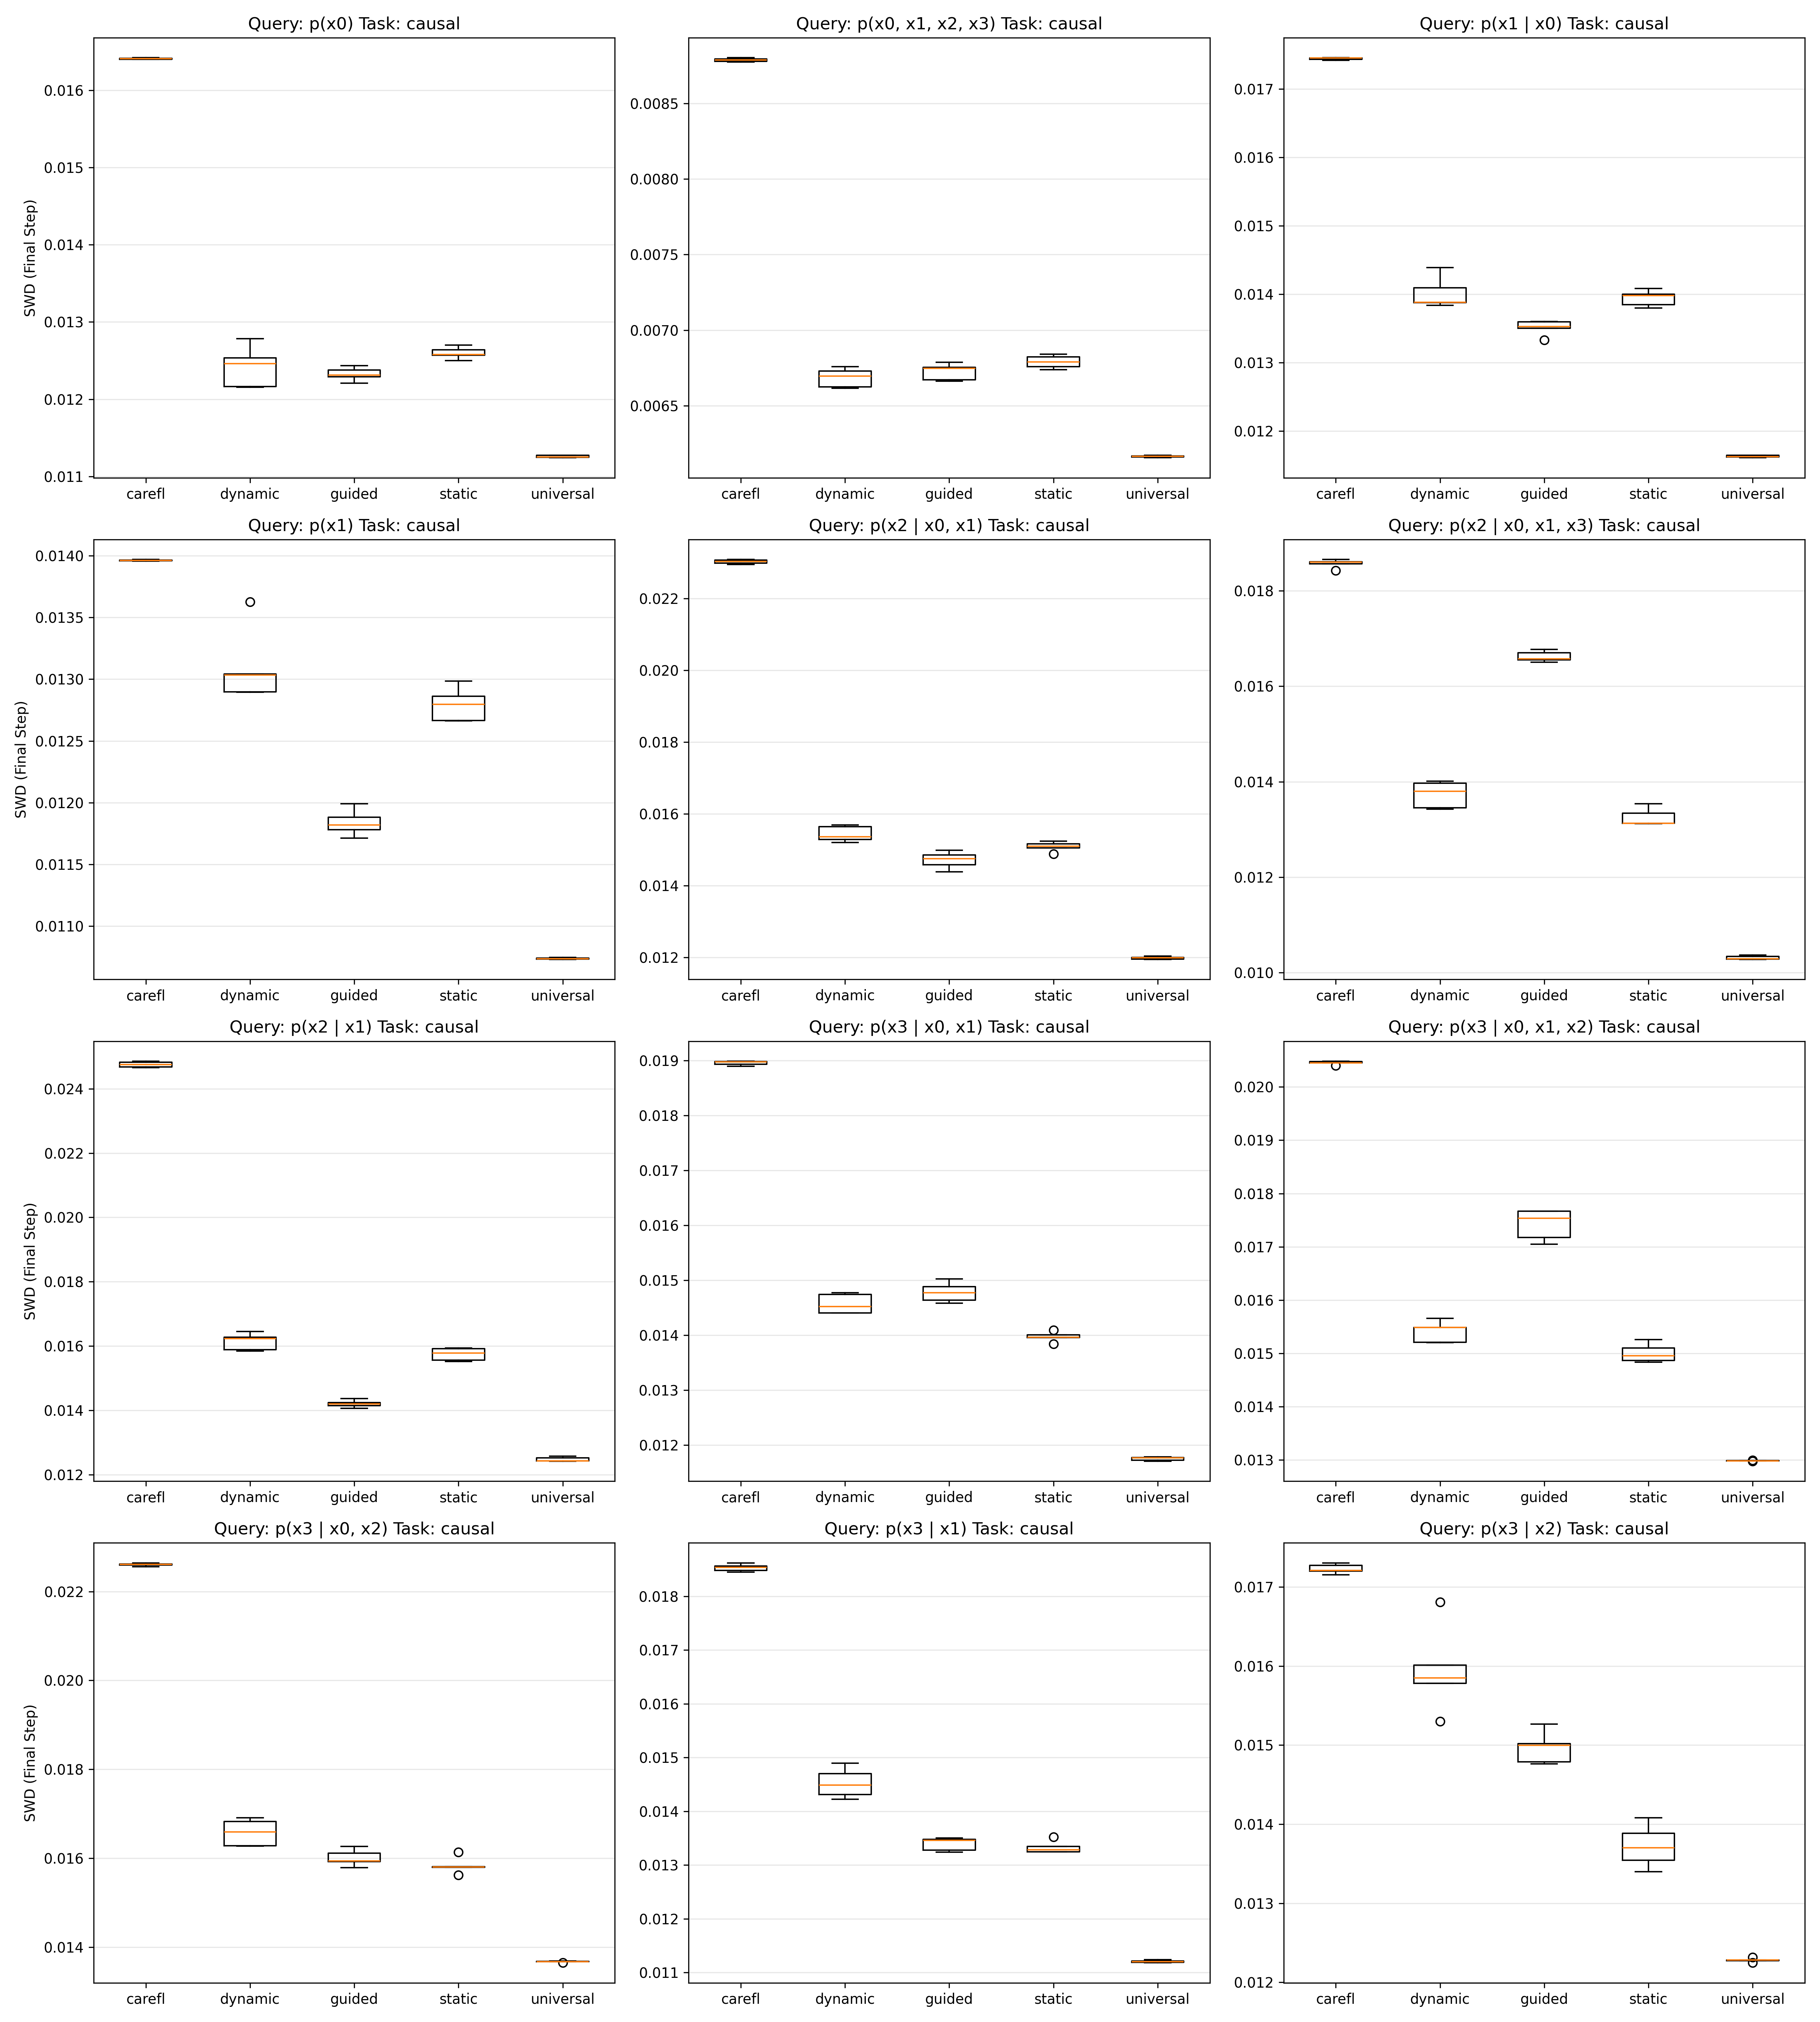
\includegraphics[width=\textwidth]{images/experimental_figures/nonlinear/final_box_swd_pgms_all_task_causal_queries_all.png}
    \caption{\textbf{Per-query breakdown of Figure~\ref{fig:pgm-results}a} (causal alignment, nonlinear $4$-node PGMs). One panel per query; each box shows the spread over $5$ learner seeds, each averaged over the $5$ PGM seeds. Read for the ranking of methods within each panel; scales differ between panels.}
    \label{fig:causal-nonlinear-pgm-queries}
\end{figure}

\begin{figure}[hbt!]
    \centering
    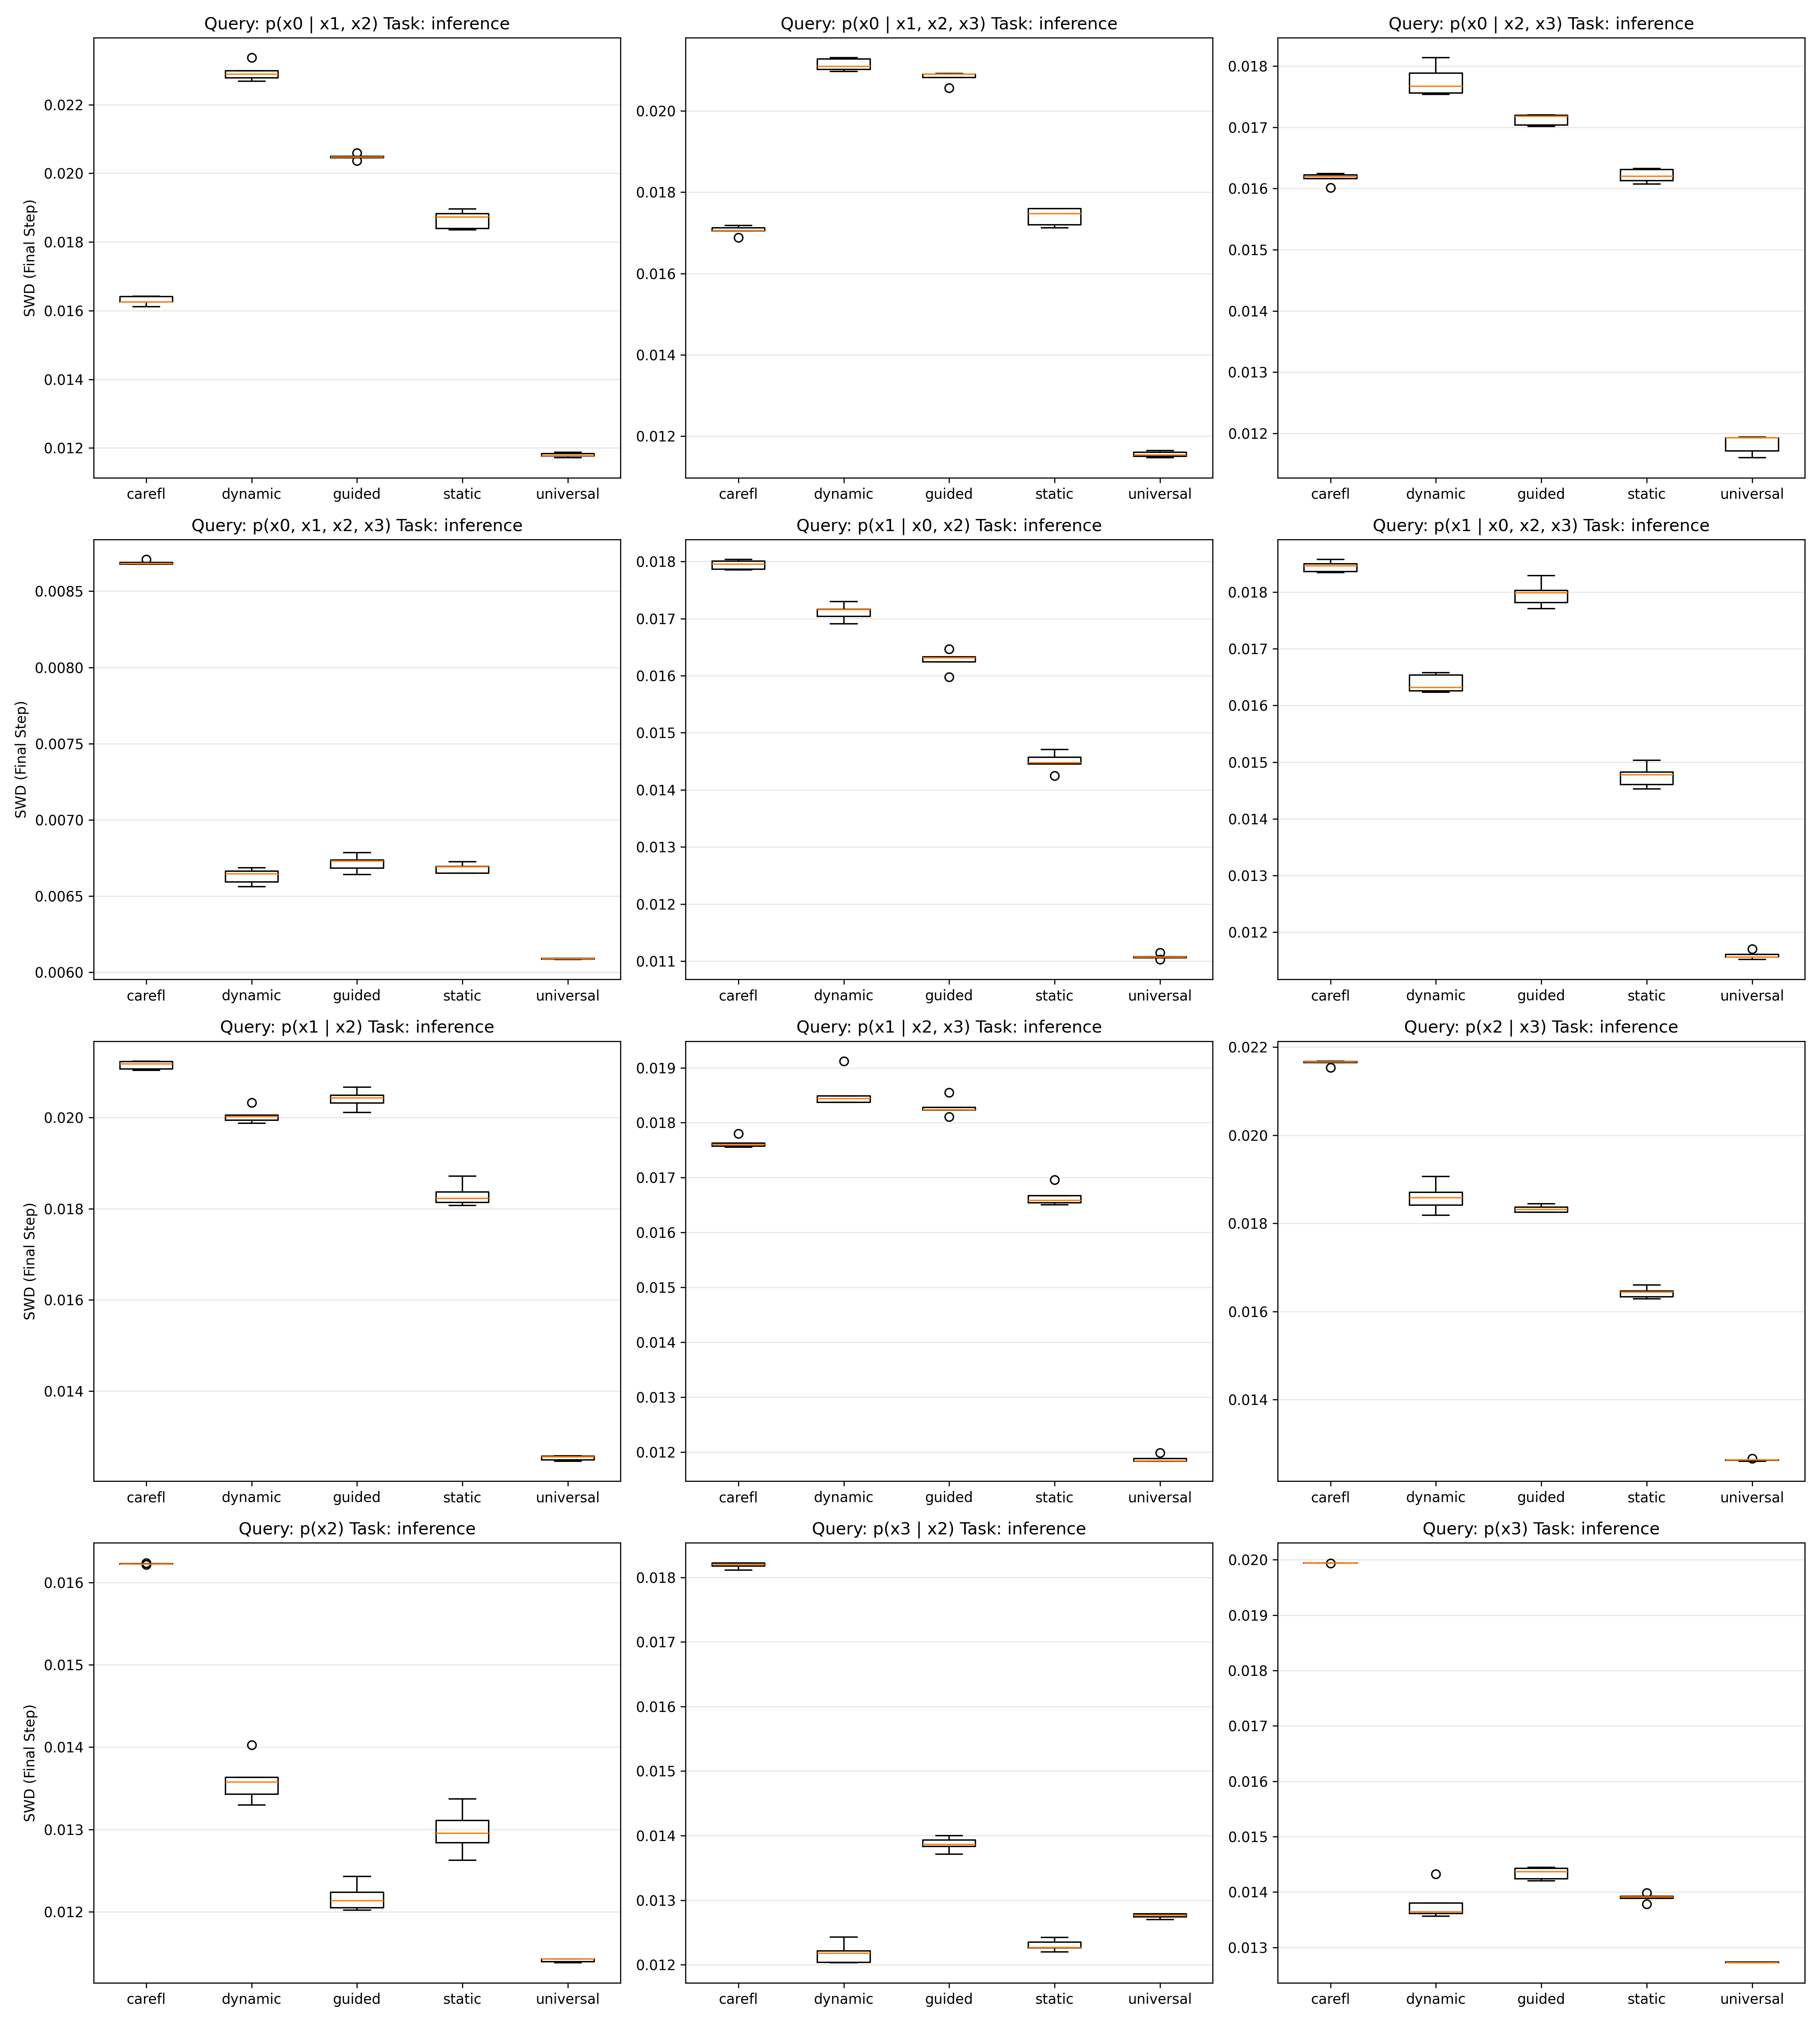
\includegraphics[width=\textwidth]{images/experimental_figures/nonlinear/final_box_swd_pgms_all_task_inference_queries_all.png}
    \caption{\textbf{Per-query breakdown of Figure~\ref{fig:pgm-results}c} (inference alignment, nonlinear $4$-node PGMs). One panel per query; each box shows the spread over $5$ learner seeds, each averaged over the $5$ PGM seeds. Read for the ranking of methods within each panel; scales differ between panels.}
    \label{fig:inference-nonlinear-pgm-queries}
\end{figure}

\subsection{Scaling to $8$-node PGMs}

To check that the framework is not limited to very small graphs, we repeat the inference evaluation on random $8$-node nonlinear PGMs ($5$ PGM seeds $\times$ $5$ learner seeds). Figure~\ref{fig:inference-n8} shows that the qualitative picture is unchanged from $n=4$\cam{: Universal is most accurate ($3.4 \times 10^{-3}$, mean over runs), static conditioning follows closely ($3.9$), and guidance, CAREFL and dynamic conditioning form a second group ($4.8$--$5.0$), the same ordering as on the $4$-node inference queries. Seed-to-seed spread is small ($\leq 0.3 \times 10^{-3}$), so the gaps between the two groups are well resolved.} This is consistent with our central finding---on well-sampled graphs, structure is a competitive but not dominant choice, and its advantage is most visible under limited data (Appendix~\ref{sec:sample-efficiency}). The binding constraint on scaling further is \emph{evaluation}, not training: generating MCMC ground truth for every conditional query grows quickly with $n$ (Section~\ref{sec:future_work}).

\begin{figure}[hbt!]
    \centering
    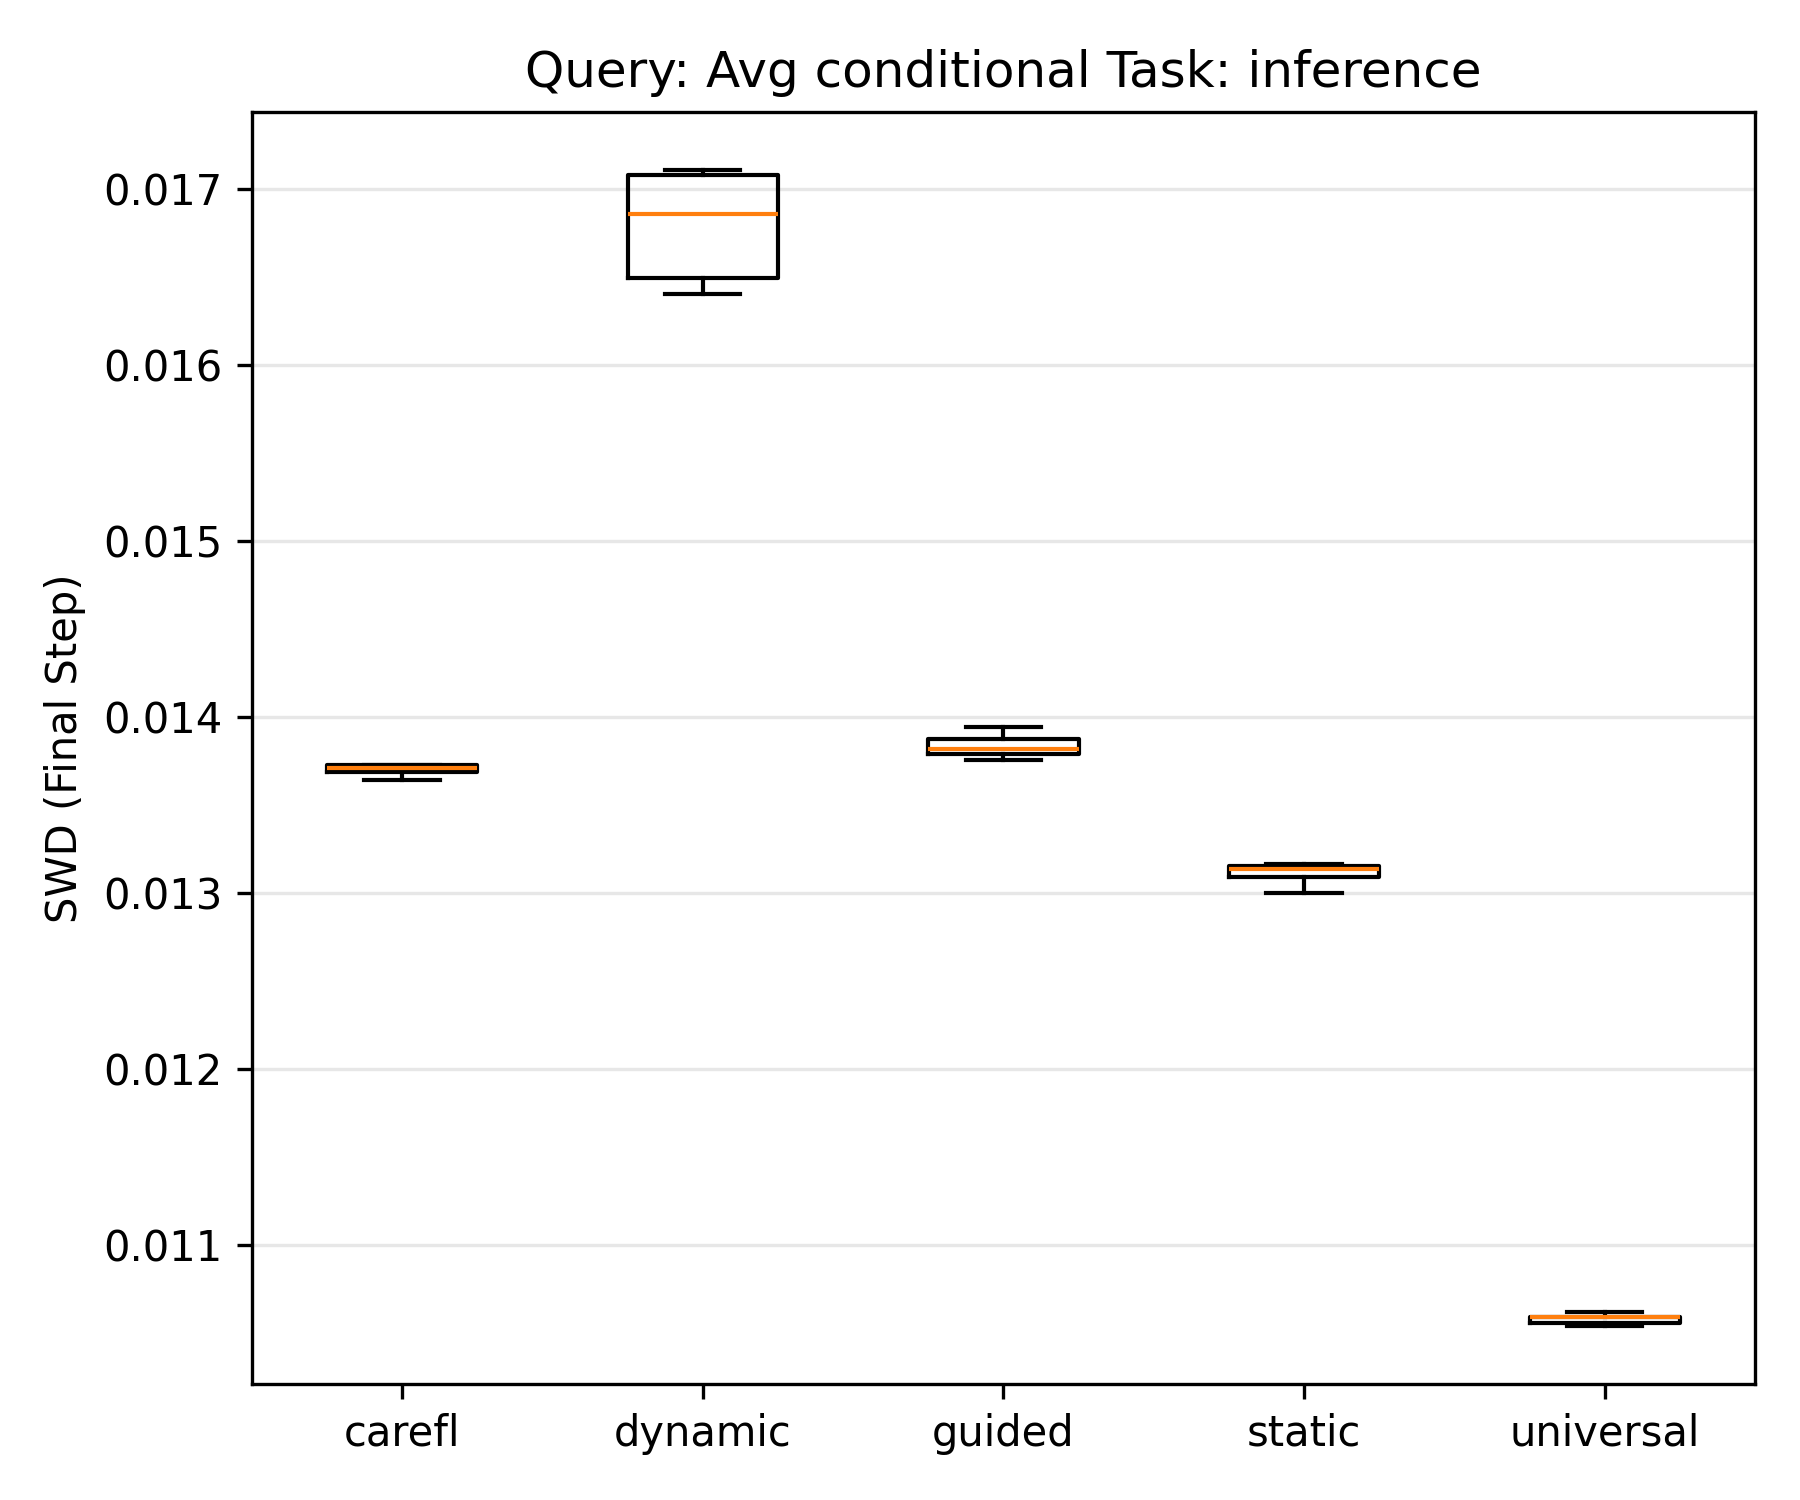
\includegraphics[width=0.7\textwidth]{images/experimental_figures/nonlinear8/final_box_swd_pgms_all_task_inference_queries_avg_conditional.png}
    \caption{\textbf{Inference on $8$-node nonlinear PGMs.} Normalized SWD on posterior queries, aggregated over conditional queries, $5$ PGM seeds and $5$ learner seeds. Universal is the structured spline flow of Section~\ref{sec:experiments}, the mechanism family that generates these PGMs. The structured (Static) flow remains competitive at $n=8$, matching the $n=4$ trend\cam{; note the $y$-axis does not start at zero}.}
    \label{fig:inference-n8}
\end{figure}

\subsection{MNIST}

\begin{figure*}[hbt!]
    \centering
    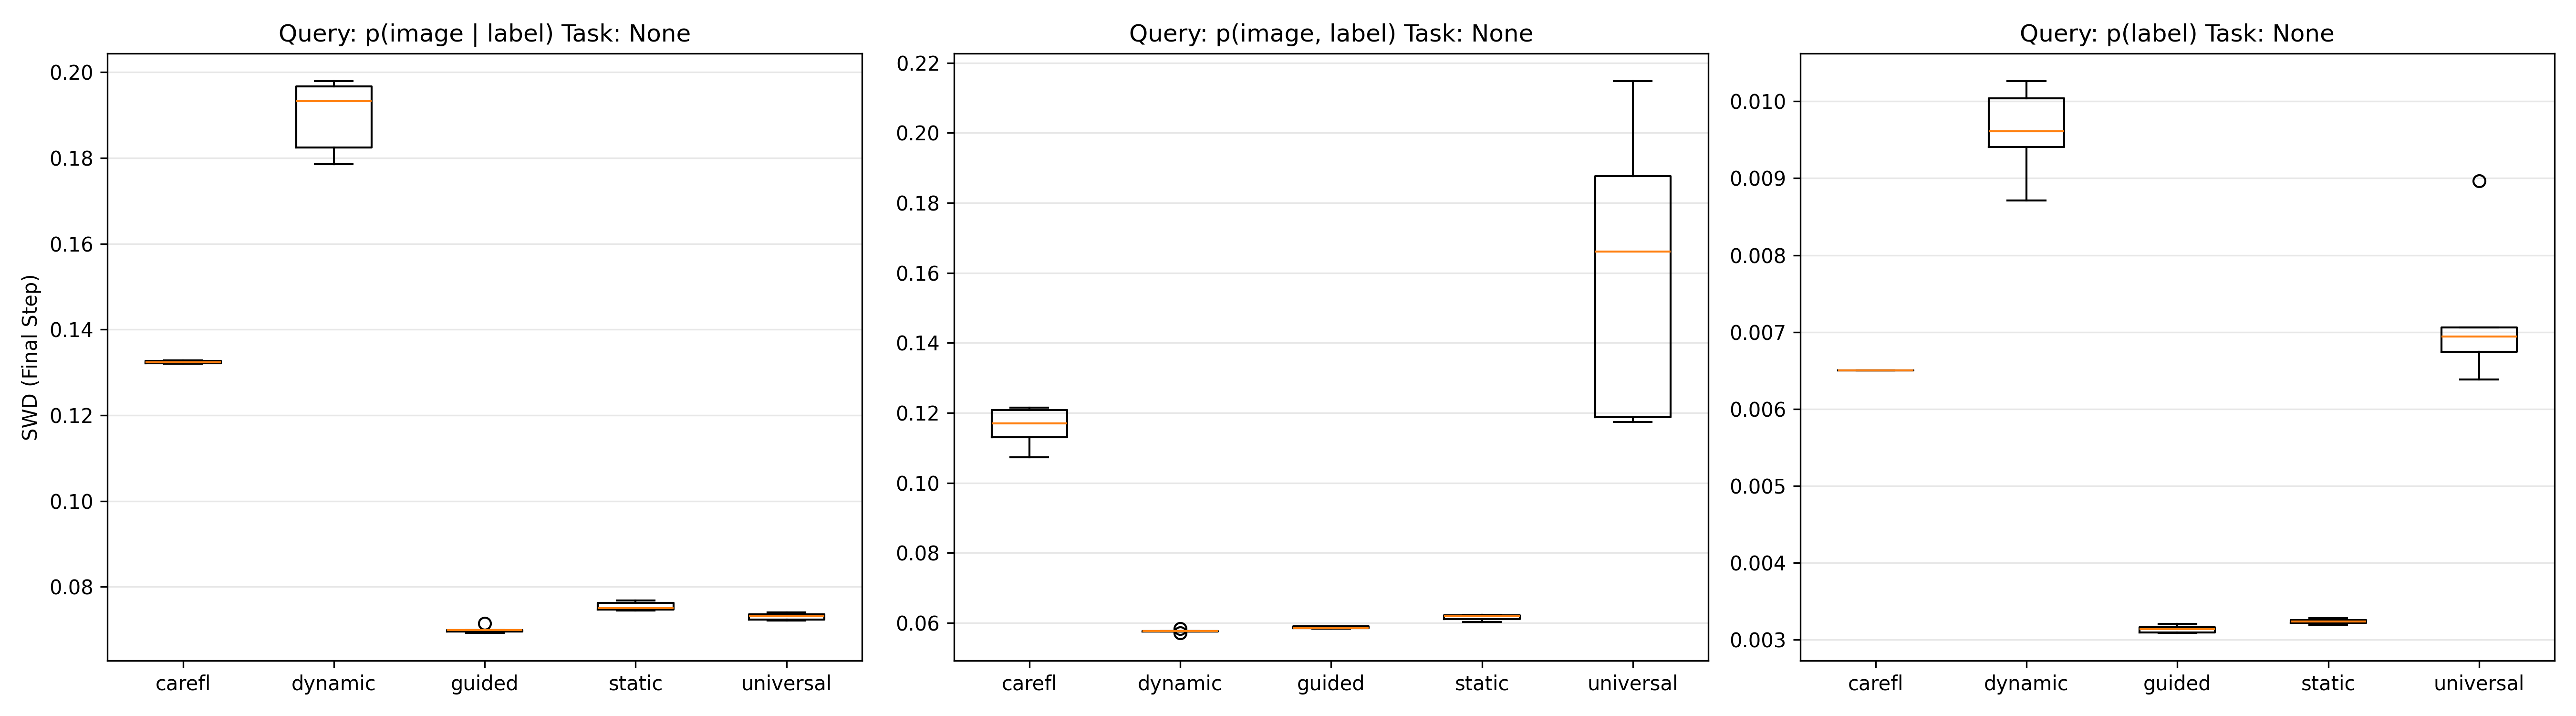
\includegraphics[width=\textwidth]{images/experimental_figures/mnist/final_box_swd_pgms_all_task_all_queries_all.png}
    \caption{\textbf{MNIST Results.} Sliced Wasserstein Distance across joint, marginal, and conditional distributions for the structure \texttt{labels}$\to$\texttt{images}. Aggregated over 5 seeds.}
    \label{fig:mnist-swd}
\end{figure*}

\begin{figure}[hbt!]
    \centering
    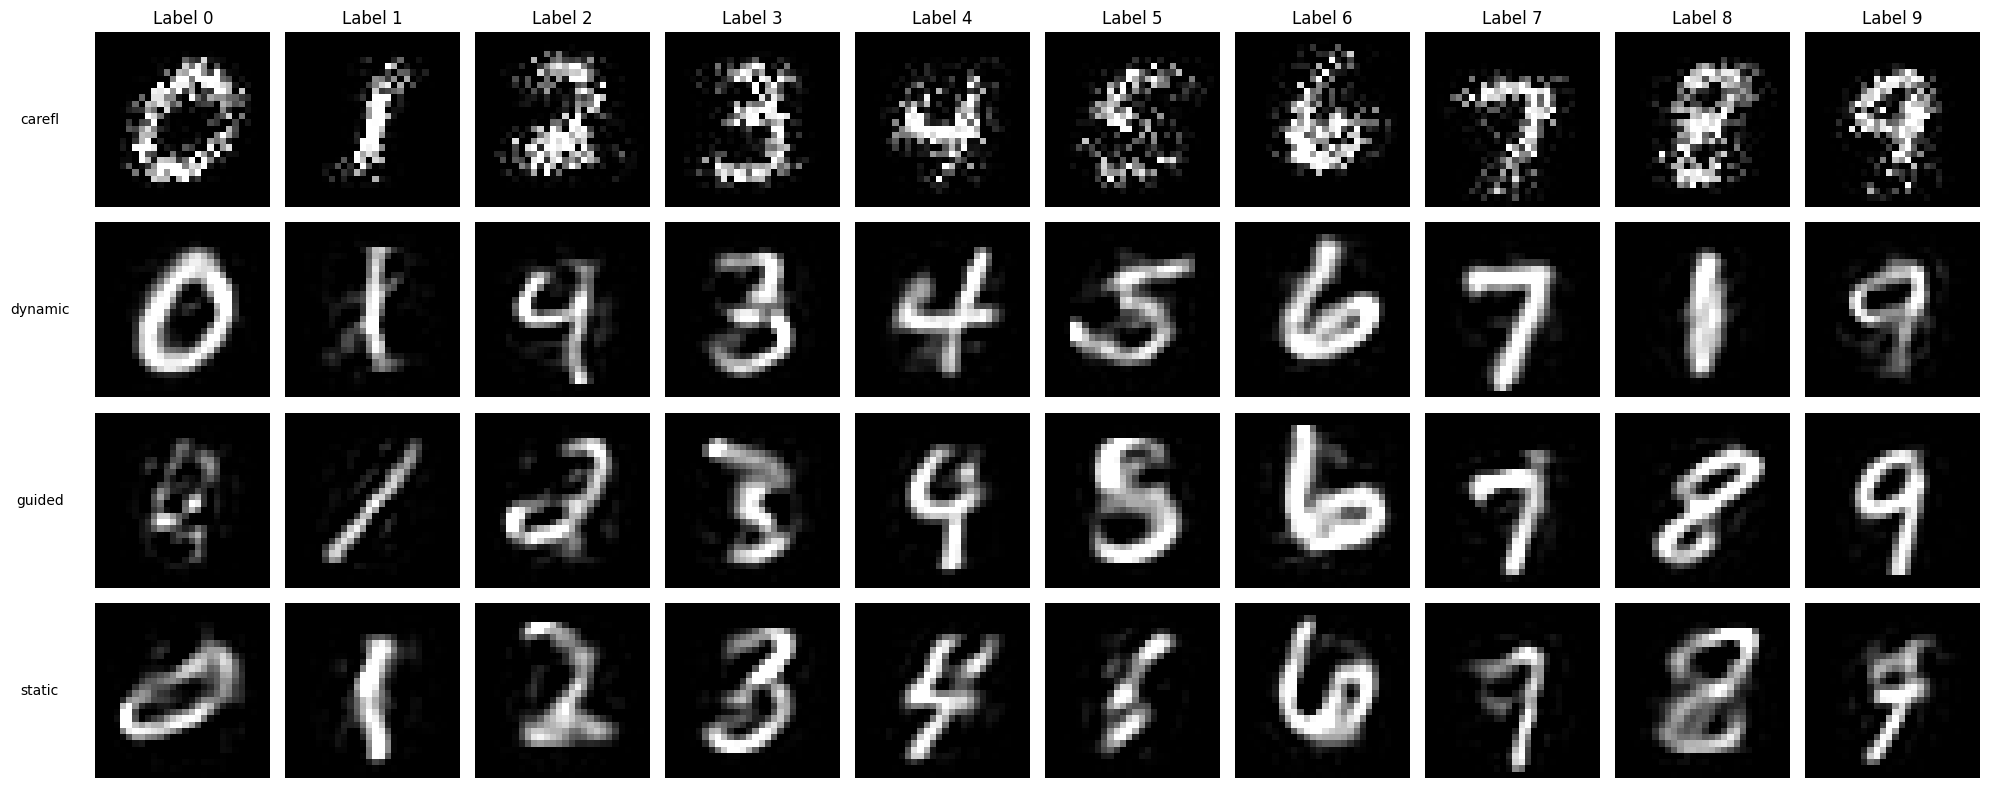
\includegraphics[width=\textwidth]{images/experimental_figures/mnist/mnist_samples1.png}
    \caption{Samples of $p(\text{image} \mid \text{label})$ from four of the MNIST models (rows: CAREFL, Dynamic, Guided, Static; columns: conditioning label), one learner seed.}
    \label{fig:mnist-sample1}
\end{figure}

\begin{figure}[hbt!]
    \centering
    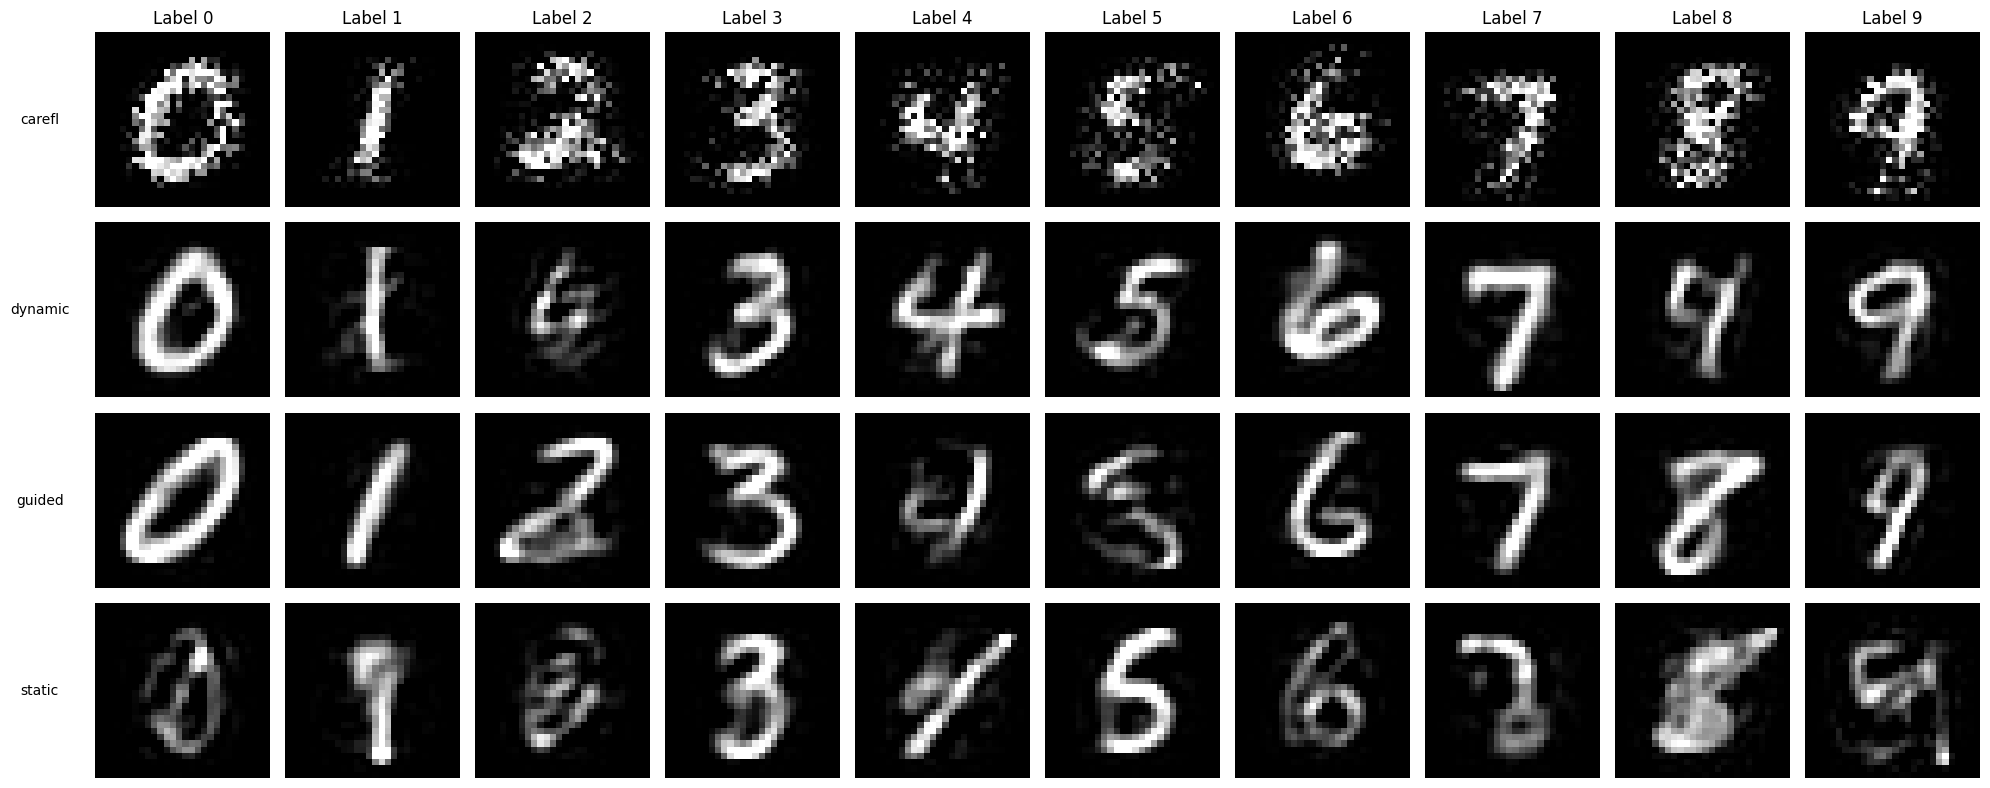
\includegraphics[width=\textwidth]{images/experimental_figures/mnist/mnist_samples2.png}
    \caption{Samples of $p(\text{image} \mid \text{label})$ from four of the MNIST models (rows: CAREFL, Dynamic, Guided, Static; columns: conditioning label), one learner seed.}
    \label{fig:mnist-sample2}
\end{figure}

\begin{figure}[hbt!]
    \centering
    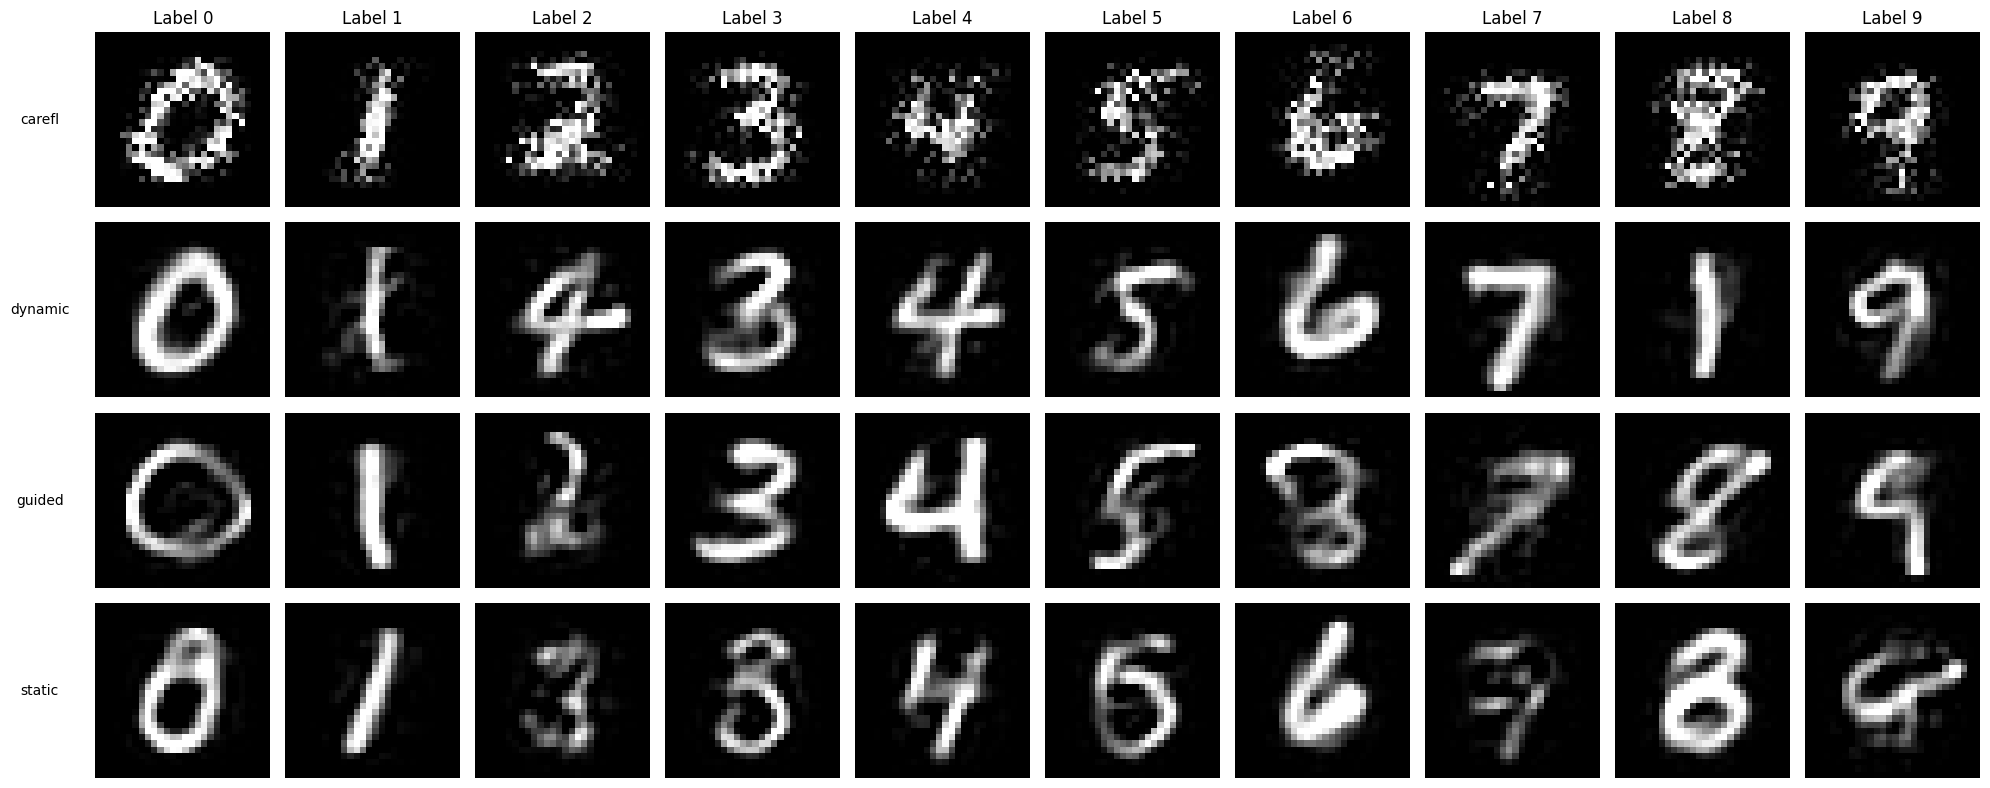
\includegraphics[width=\textwidth]{images/experimental_figures/mnist/mnist_samples3.png}
    \caption{Samples of $p(\text{image} \mid \text{label})$ from four of the MNIST models (rows: CAREFL, Dynamic, Guided, Static; columns: conditioning label), one learner seed.}
    \label{fig:mnist-sample3}
\end{figure}


\end{document}
